%%____________________________________________________________________________||
\section{Interpretation in Simplified SUSY models}
\label{sec:susy}

To interpret the results of this search, simplified
%models~\cite{Alwall:2008ag,Alwall:2008va,Alves:2011wf} for the production of
supersymmetric particles are considered.  They use only a limited set
of sparticles in the production and decay and enable comprehensive
studies of individual SUSY event topologies. These studies can be
performed in terms of fundamental properties such as decay modes,
production cross sections and sparticle masses.

\subsection{Signal models}
\label{sec:susy_models}
Interpretations are presented for pair production of gluino, stop, sbottom and
squark particles with several different possibilities for the decay
chain. The simplified models used in the analysis are summarised in
Tab.~\ref{tab:simplified-models}. Benchmark points are also listed, which will
be used throughout the section. Two benchmarks are provided, where relevant,
to cover the phenomenology of compressed and uncompressed spectra. All the
benchmarks are chosen to be right within the expected exclusion. \\
%A sensitivity study has been performed on these benchmark models, which is
%described in App.~\ref{app:sensitivity-benchmarks}. 

Sketches of the production and decay in these models are shown in
Figs.~\ref{fig:simplified-models-feyn-light}-\ref{fig:simplified-models-feyn-3rdGen}.
Systematic uncertainties on the signal acceptance are detailed in
Sec.~\ref{sec:sig-syst}.

All the models are generated using the FastSim package
\cite{Abdullin:2011zz}.  FastSim Monte Carlo samples are corrected
using FastSim-to-FullSim scale factor, accounting for difference in
b-tag efficiency. These scale factors are applied on top of the
FullSim scale factors applied for the other Monte Carlo samples.

\begin{table}[h!]
    \scriptsize
    \caption{A summary of the simplified models used in this analysis.}
    \label{tab:simplified-models}
    \centering
    \begin{tabular}{ lllllll }
        \hline \hline
        Model & Production & Decay & Previous limits & Figure & Benchmarks $(m_{\mathrm{Susy}},m_{\mathrm{LSP}})$ \\ 
        \hline \hline
        T1qqqq & \ppToGluGlu & \gluToQQNo & $m_{\mathrm{Gluino}}>\sim 1550 \,\mathrm{GeV}$ (ICHEP) & \ref{fig:T1qqqq_feyn} & \parbox[t]{3.5cm}{Compressed: (1000,850)\\Uncompressed: (1700,100)} \\
        \hline
        T1bbbb & \ppToGluGlu & \gluToBBNo & $m_{\mathrm{Gluino}}>\sim 1850 \,\mathrm{GeV}$ (ICHEP) & \ref{fig:T1bbbb_feyn} & \parbox[t]{3.5cm}{Compressed: (1300,1100)\\Uncompressed: (1900,100)} \\
        \hline
        T1tttt & \ppToGluGlu & \gluToTTNo & $m_{\mathrm{Gluino}}>\sim 1600 \,\mathrm{GeV}$ (ICHEP) & \ref{fig:T1tttt_feyn} & \parbox[t]{3.5cm}{Compressed: (950,600)\\Uncompressed: (1700,100)} \\
        \hline
        T2qq (1-fold) & \ppToSquaSqua & \squarkToQ & $m_{\mathrm{Squark}}>\sim 650 \,\mathrm{GeV}$ (2015) & \ref{fig:T2qq_feyn} & \parbox[t]{3.5cm}{Compressed: (400,300)\\Uncompressed: (700,100)} \\
        \hline
        T2qq (8-fold) & \ppToSquaSqua & \squarkToQ & $m_{\mathrm{Squark}}>\sim 1075 \,\mathrm{GeV}$ (2015) & \ref{fig:T2qq_feyn} & \parbox[t]{3.5cm}{Compressed: (700,600)\\Uncompressed: (1250,100)} \\
        \hline
        T2bb   & \ppToSbotSbot & \sbottomToB & $m_{\mathrm{Sbottom}}>\sim 980 \,\mathrm{GeV}$ (ICHEP)& \ref{fig:T2bb_feyn} & \parbox[t]{3.5cm}{Compressed: (550,450)\\Uncompressed: (1000,100)} \\
        \hline
        T2tt   & \ppToStopStop & \stopToTNo & $m_{\mathrm{Stop}}>\sim 925 \,\mathrm{GeV}$ (ICHEP) & \ref{fig:T2tt_feyn} & \parbox[t]{3.5cm}{Compressed: (450,200)\\Uncompressed: (1000,50)\\$W$ corridor: (250,150)} \\
        \hline
        T2cc   & \ppToStopStop & \stopToCNo & $m_{\mathrm{Stop}}>\sim 350 \,\mathrm{GeV}$ (2015)& \ref{fig:T2cc_feyn} & Compressed: (500,480) \\
        \hline \hline
    \end{tabular}
\end{table}

\begin{figure}[h!]
    \begin{center}
        \subfigure[T1qqqq]{
            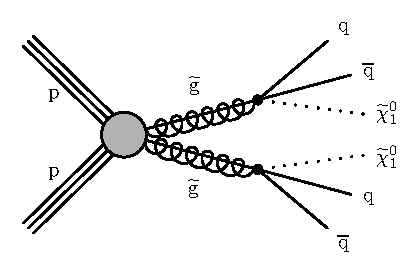
\includegraphics[width=0.3\textwidth]{figures/susyResults/T1qqqq_feyn}
            \label{fig:T1qqqq_feyn}
        }~~
        \subfigure[T2qq]{
            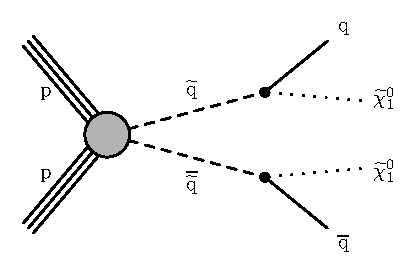
\includegraphics[width=0.3\textwidth]{figures/susyResults/T2qq_feyn}
            \label{fig:T2qq_feyn}
        }~~
        \caption{
            Graphical representation of the production and decay of
            supersymmetric particles in ``light-flavour models'', i.e. with
            gluinos/squarks decaying to light quarks.
        }
        \label{fig:simplified-models-feyn-light}
    \end{center}
\end{figure}

\begin{figure}[h!]
    \begin{center}
        \subfigure[T1bbbb]{
            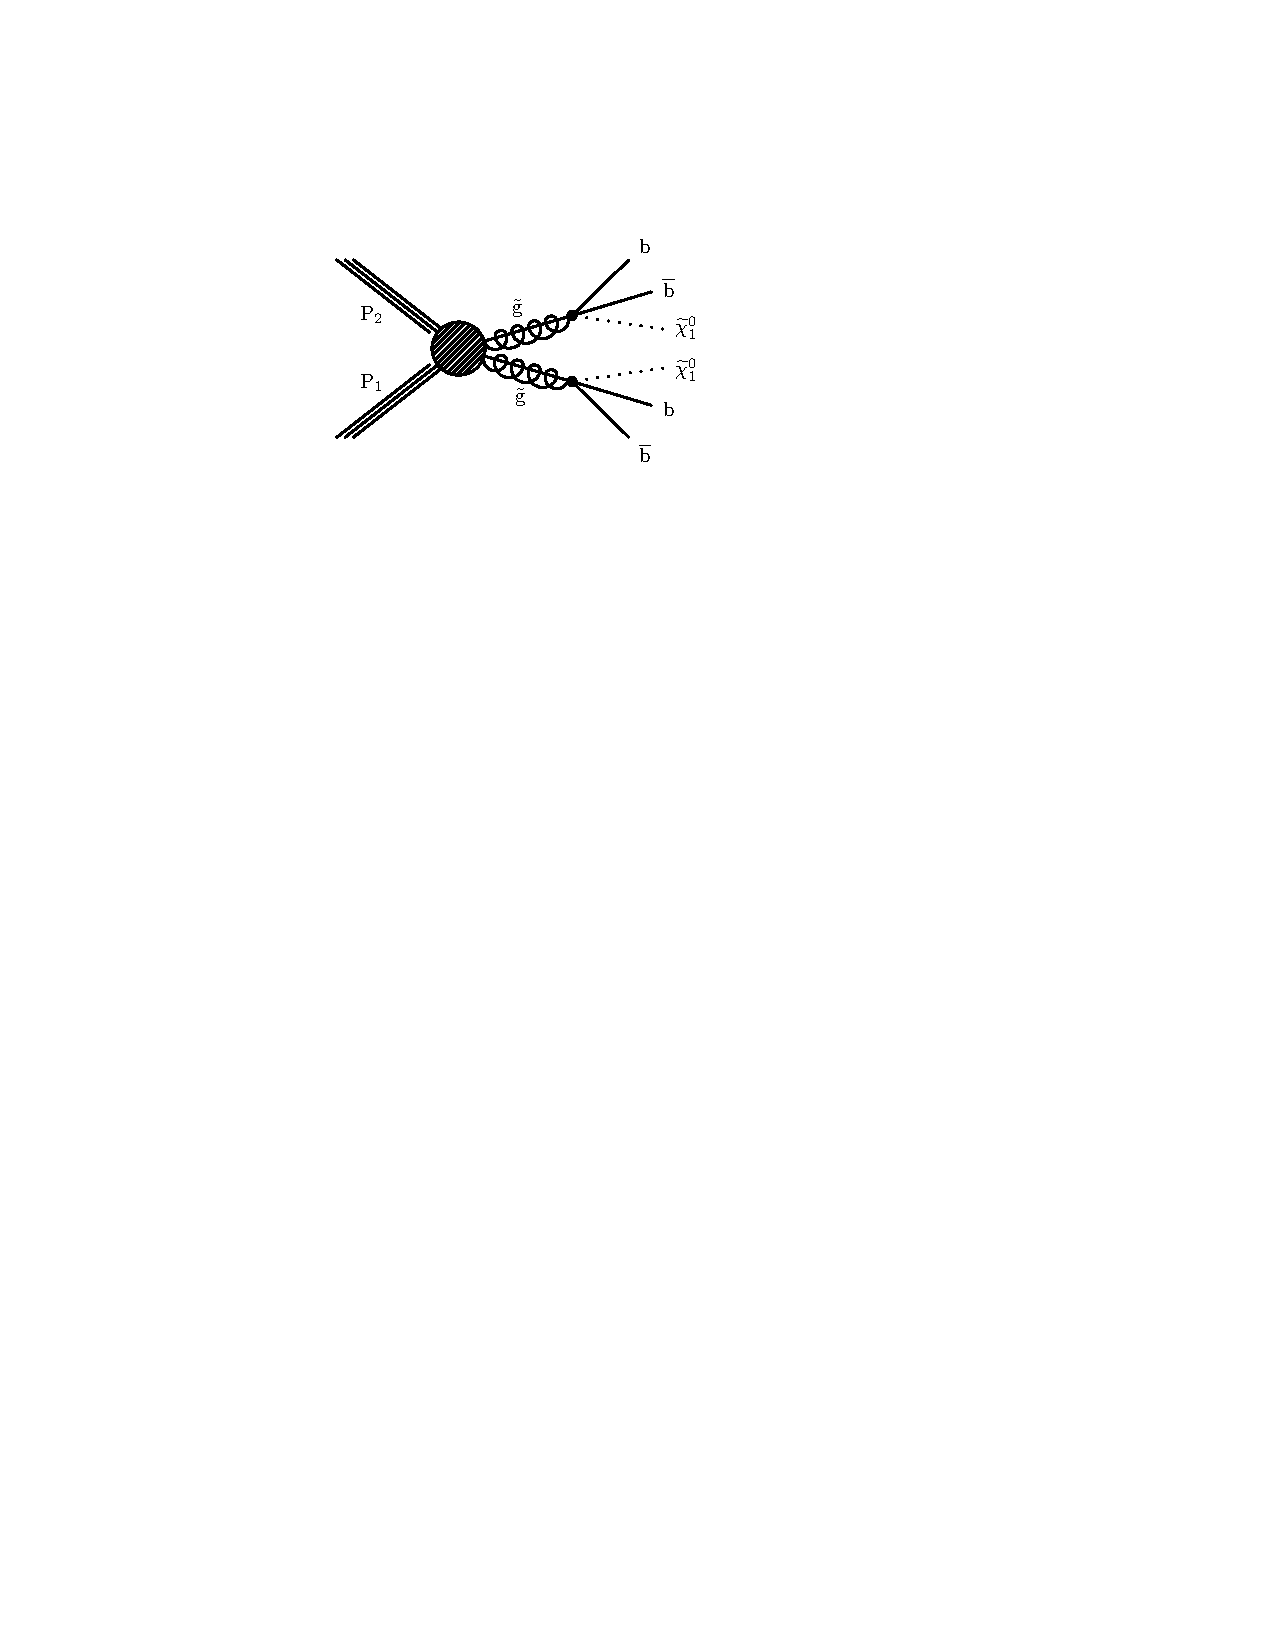
\includegraphics[width=0.3\textwidth]{figures/susyResults/T1bbbb_feyn}
            \label{fig:T1bbbb_feyn}
        }~~
        \subfigure[T1tttt]{
            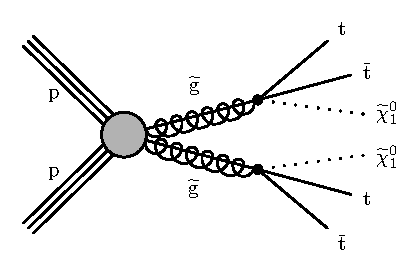
\includegraphics[width=0.3\textwidth]{figures/susyResults/T1tttt_feyn}
            \label{fig:T1tttt_feyn}
        }~~
        \caption{
            Graphical representation of the production and decay of
            supersymmetric particles in gluino models with decoupled third
            generation squarks.
        }
        \label{fig:simplified-models-feyn-gluino}
    \end{center}
\end{figure}

\begin{figure}[h!]
    \begin{center}
        \subfigure[T2bb]{
            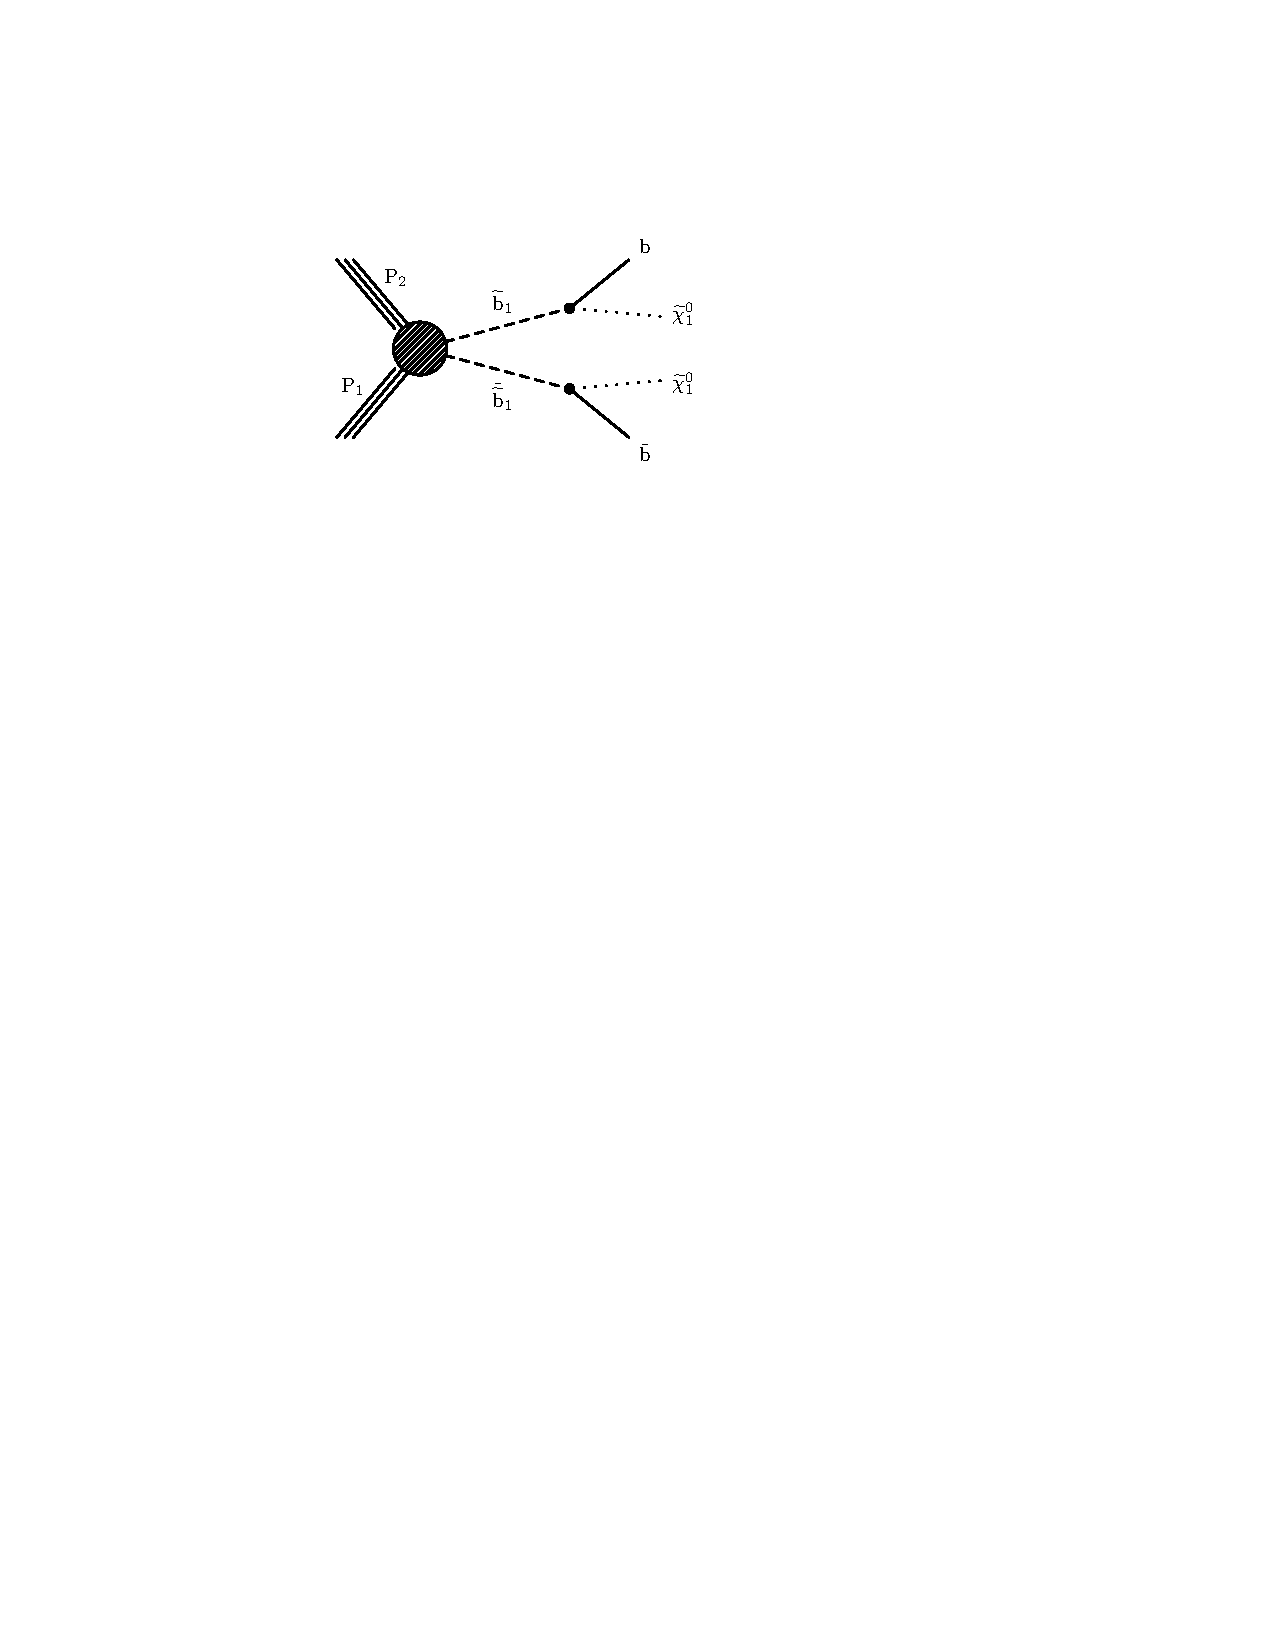
\includegraphics[width=0.3\textwidth]{figures/susyResults/T2bb_feyn}
            \label{fig:T2bb_feyn}
        }~~
        \subfigure[T2tt]{
            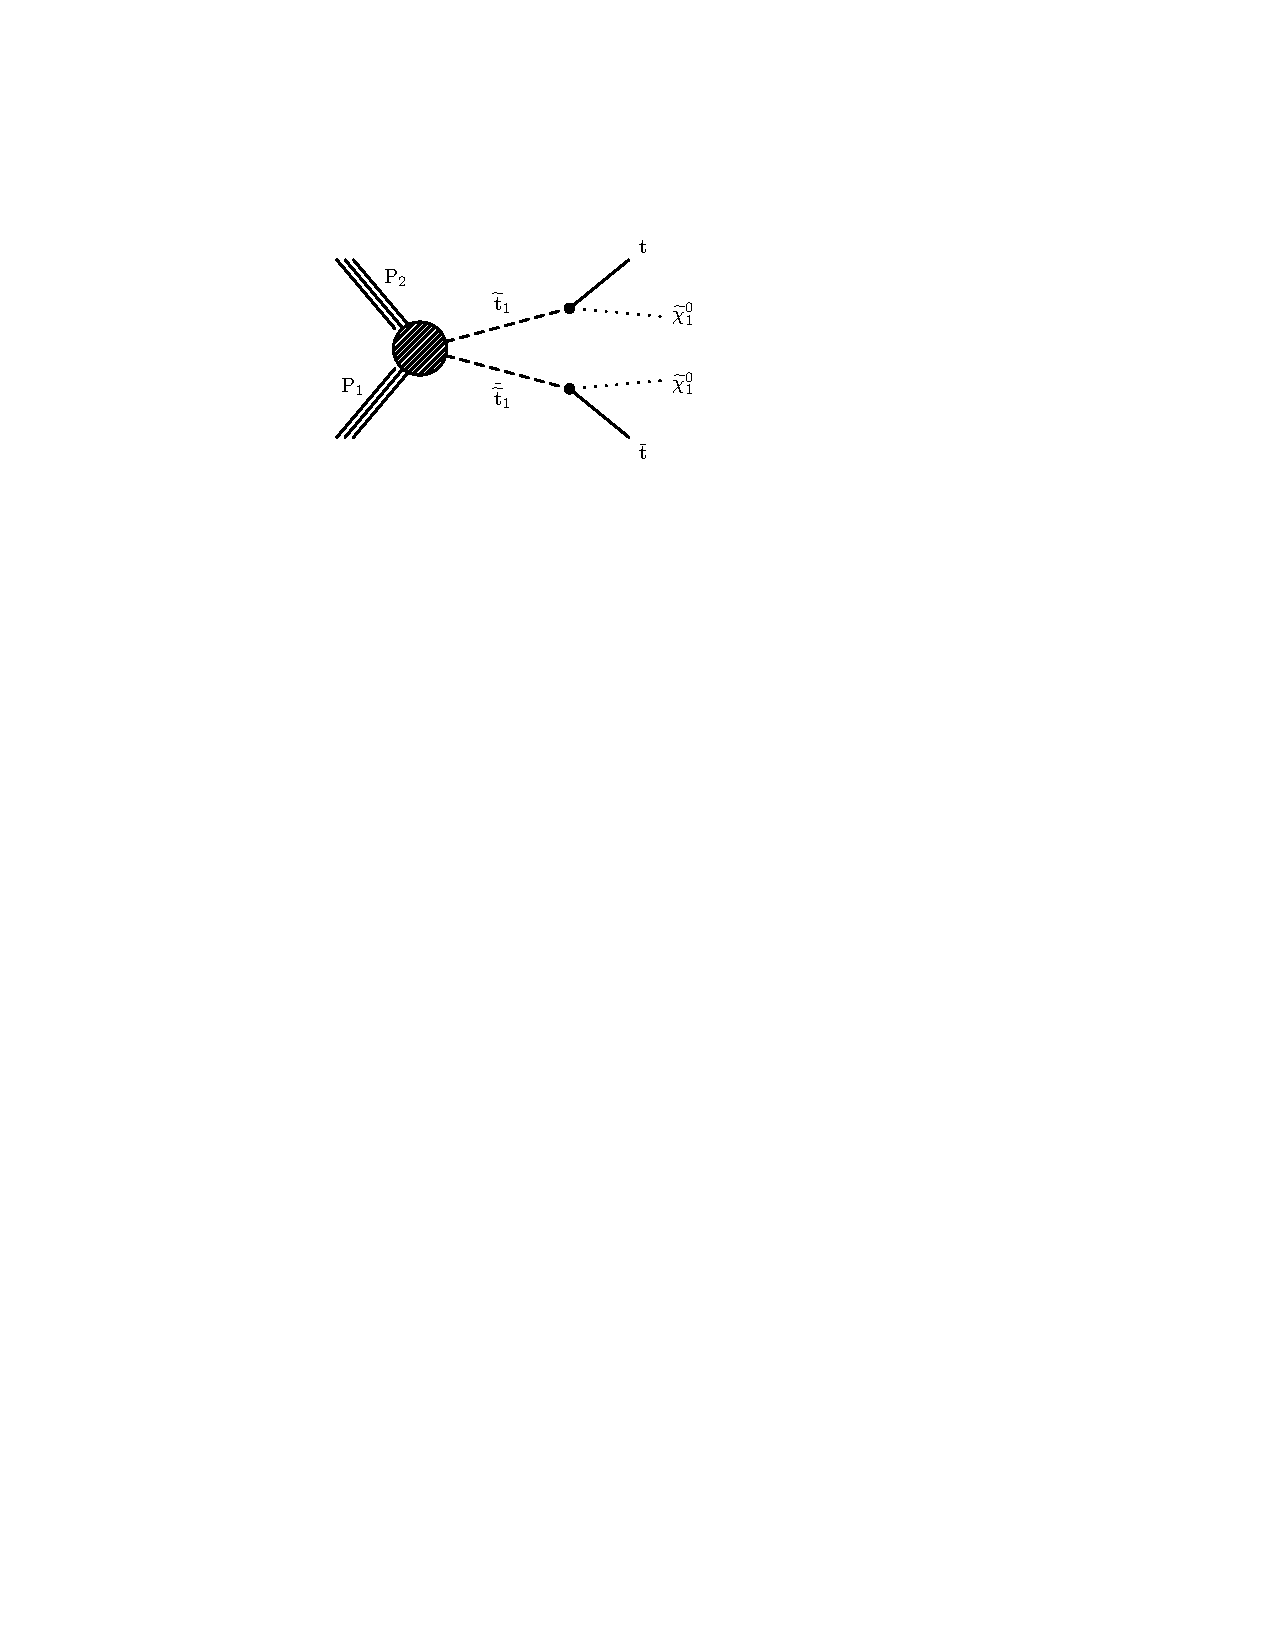
\includegraphics[width=0.3\textwidth]{figures/susyResults/T2tt_feyn}
            \label{fig:T2tt_feyn}
        }~~
        \subfigure[T2cc]{
            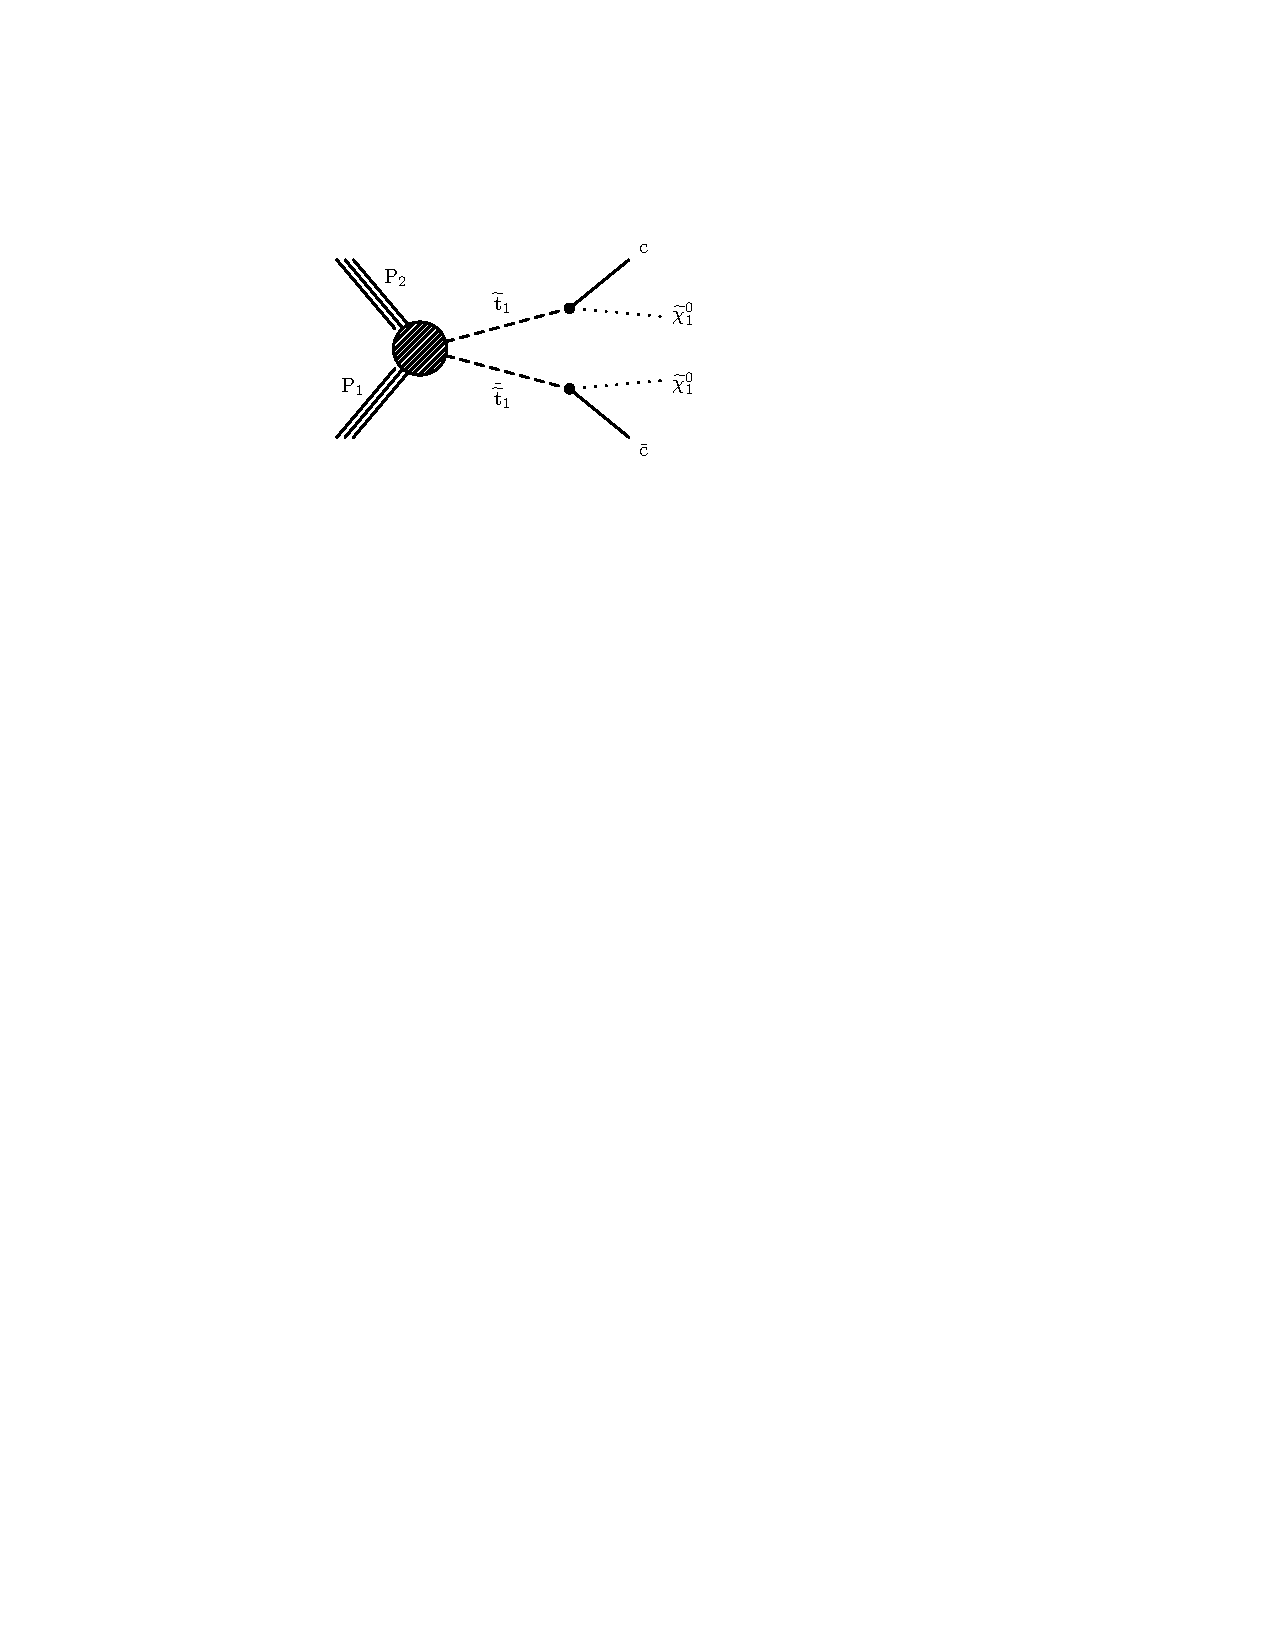
\includegraphics[width=0.3\textwidth]{figures/susyResults/T2cc_feyn}
            \label{fig:T2cc_feyn}
        }~~
        \caption{
            Graphical representation of the production and decay of
            supersymmetric particles in models with the production of third
            generation squarks (stops and sbottomes).
        }
        \label{fig:simplified-models-feyn-3rdGen}
    \end{center}
\end{figure}

\clearpage
\subsection{Signal acceptance times efficiency}
\label{sec:sig-accept-contam}

In Tab. \ref{tab:sig-eff} the signal efficiency for benchmark mass
points for all the models is summarised. The signal efficiency across
the whole ($m_{\mathrm{Susy}},m_{\mathrm{LSP}}$) for the simplified
models used in the analysis is shown in
Figs.~\ref{fig:T1qqqq_eff}-\ref{fig:T2cc_eff}.

\begin{table}[h!]
    \scriptsize
    \caption{Signal efficiency for compressed and uncompressed models used in
        the analysis.}
    \label{tab:sig-eff}
    \centering
    \begin{tabular}{ lllll }
        \hline \hline
        Model & $(m_{\mathrm{Susy}},m_{\mathrm{LSP}})$ & Efficiency (total) \\ 
        \hline
        \multirow{2}{*}{T1qqqq}
            & (1700,100) & 21.1\% \\
            & (1000,850) & 9.6\% \\
        \hline
        \multirow{2}{*}{T1bbbb}
            & (1900,100)  & 25.1\% \\
            & (1300,1100) & 14.6\% \\
        \hline
        \multirow{2}{*}{T1tttt}
            & (1700,100) & 6.9\% \\
            & (950,600)  & 0.31\% \\
        \hline
        \multirow{2}{*}{T2qq (1-fold)}
            & (700,100) & 32.9\% \\
            & (400,300) & 4.5\% \\
        \hline
        \multirow{2}{*}{T2qq (8-fold)}
            & (1250,100) & 42.9\% \\
            & (700,600)  & 7.7\% \\
        \hline
        \multirow{2}{*}{T2bb}
            & (1000,100) & 40.1\% \\
            & (550,450)  & 5.7\% \\
        \hline
        \multirow{2}{*}{T2tt}
            & (1000,50) & 23.8\% \\
            & (450,200) & 4.2\% \\
            & (250,150) & 0.27\% \\
        \hline
        T2cc
            & (500,480) & 20.5\% \\
        \hline \hline
    \end{tabular}
\end{table}

%The level of signal contamination in the control regions is expected to be
%negligible for most of the models that are targeted by this search. The
%requirement of one muon or two muons in the \mj and \mmj respectively ensures
%that the control regions are depleted from signal events, in the case where the
%final state is all-hadronic. The only partial exception is the stop pair
%production followed by decay into top quarks, called T2tt. In this case, when
%top decays leptonically, a residual signal contamination may be found in the
%muon control regions. However, the kinematic selection applied to the control
%regions, like the absence of any \alt cut and the $m_{T}$ cut, helps to reduce
%the signal contamination. \\
%The metric that is chosen to study the signal contamination in the following is
%the double-ratio $(S_{SR}/B_{SR})/(S_{CR}/B_{CR})$, as the sensitivity of the
%control region ($S_{CR}/B_{CR}$) is expected to be small compared to the one in
%the signal region ($S_{SR}/B_{SR}$) by definition.
%
%Fig.~\ref{fig:contamination_T2tt} characterises the level of signal
%contamination for the T2tt ($m_{\mathrm{Stop}}=XXX$ GeV, $m_{\mathrm{LSP}}=YYY$ GeV)
%model, as a function of event category and \scalht bin. This benchmark point
%has $m_{\mathrm{Susy}}-m_{\mathrm{LSP}} \sim m_{\mathrm{top}}$, which is the
%scenario where the largest signal contamination is expected, since the
%kinematics is similar to the top quark production, which is more likely to
%satisfy the control region selection with respect to the signal region. \\
%Fig. ~\ref{fig:contamination_T2tt_yields_had} and
%~\ref{fig:contamination_T2tt_yields_had} show the expected signal yield counts
%in the signal region and \mj control region respectively, for the T2tt benchmark
%model. Fig.~\ref{fig:contamination_T2tt_relEff} shows the ratio of signal
%contamination to signal efficiency of the signal region, for the T2tt benchmark
%model. Fig.~\ref{fig:contamination_T2tt_doubleRatio} shows the ratio of
%sensitivity in the control region to the sensitivity in the signal region, for
%T2tt benchmark model. The sensitivity is defined as the ratio of signal to
%background expected counts.

%\begin{figure}[h!]
%    \begin{center}
%        \subfigure[Expected counts in the signal region]{
%            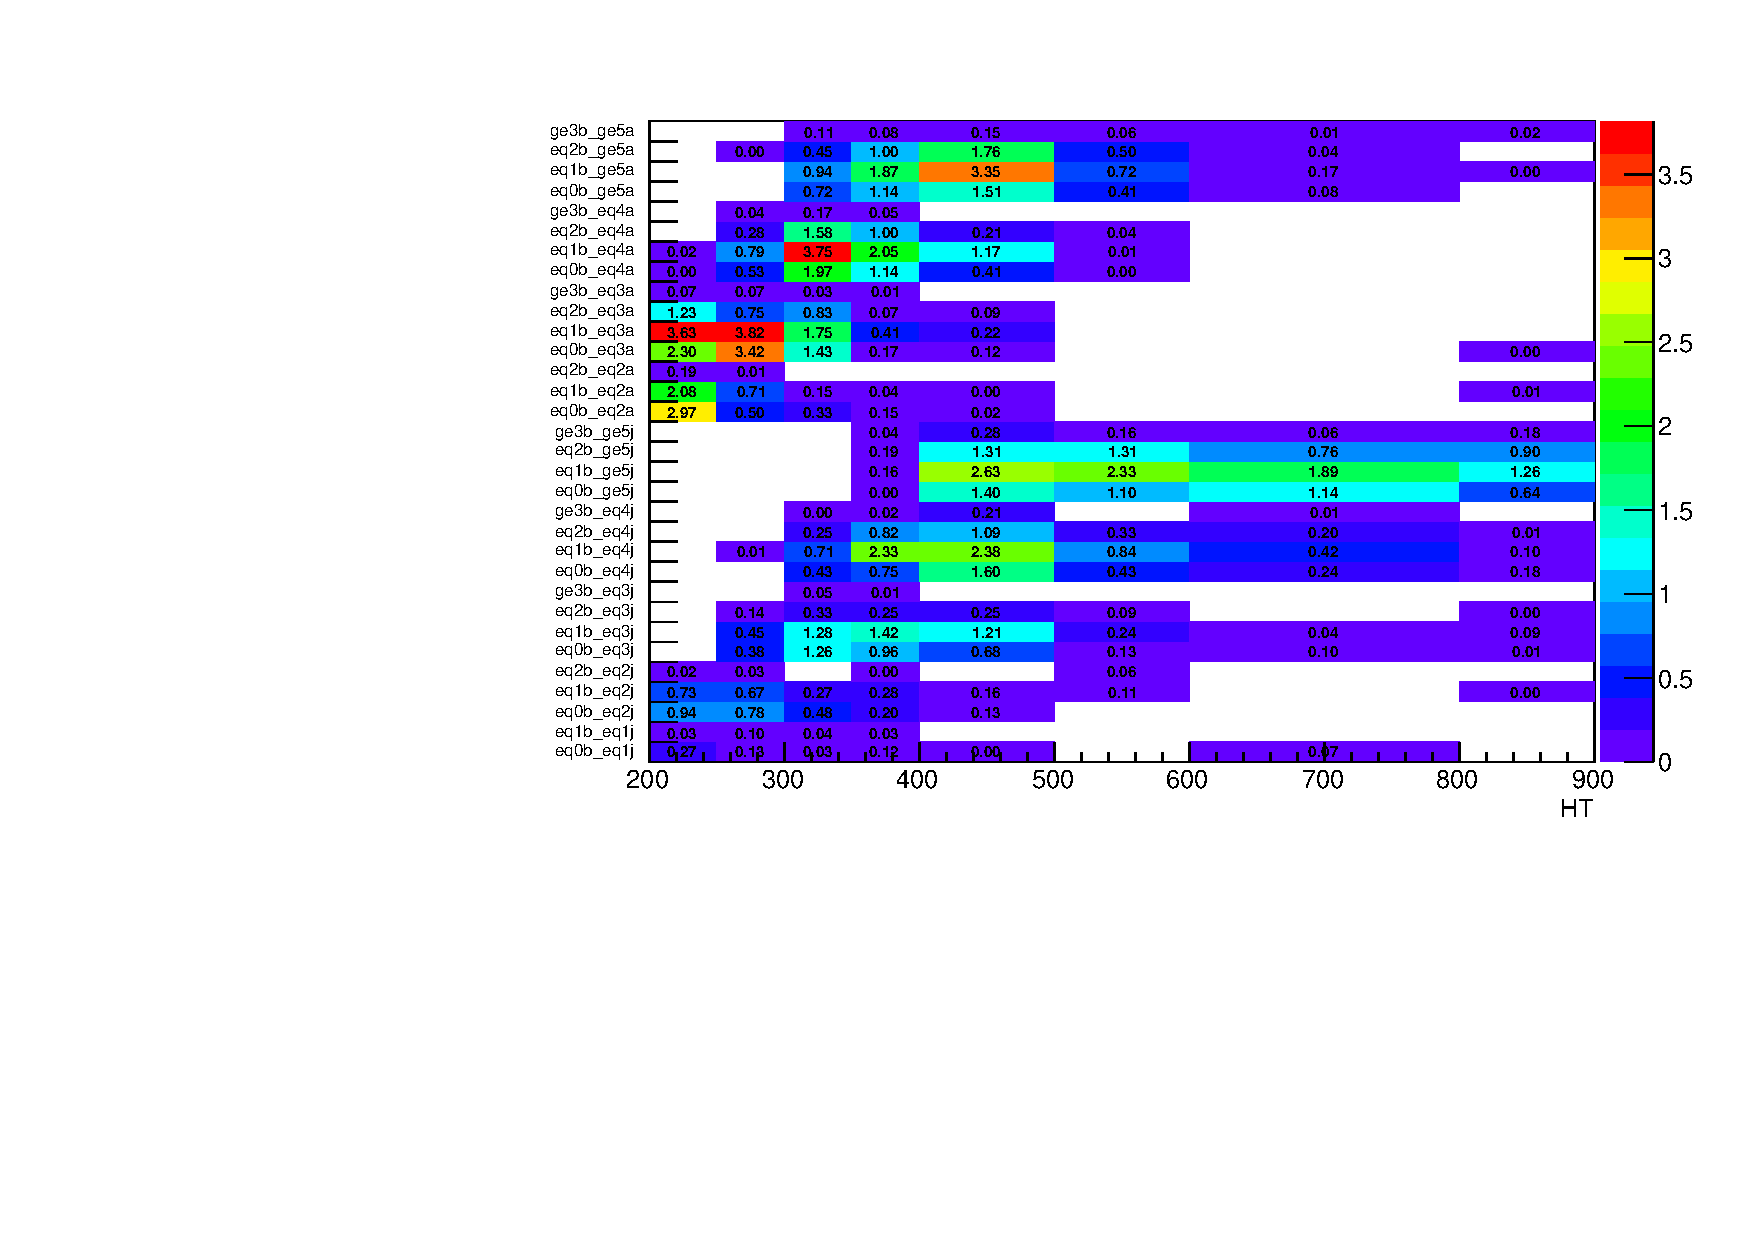
\includegraphics[width=0.5\textwidth]{figures/susyResults/sigYields_had_SMS-T2tt_mStop-250_mLSP-50_25ns}
%            \label{fig:contamination_T2tt_yields_had}
%        }
%        \subfigure[Expected counts in the \mj control region]{
%            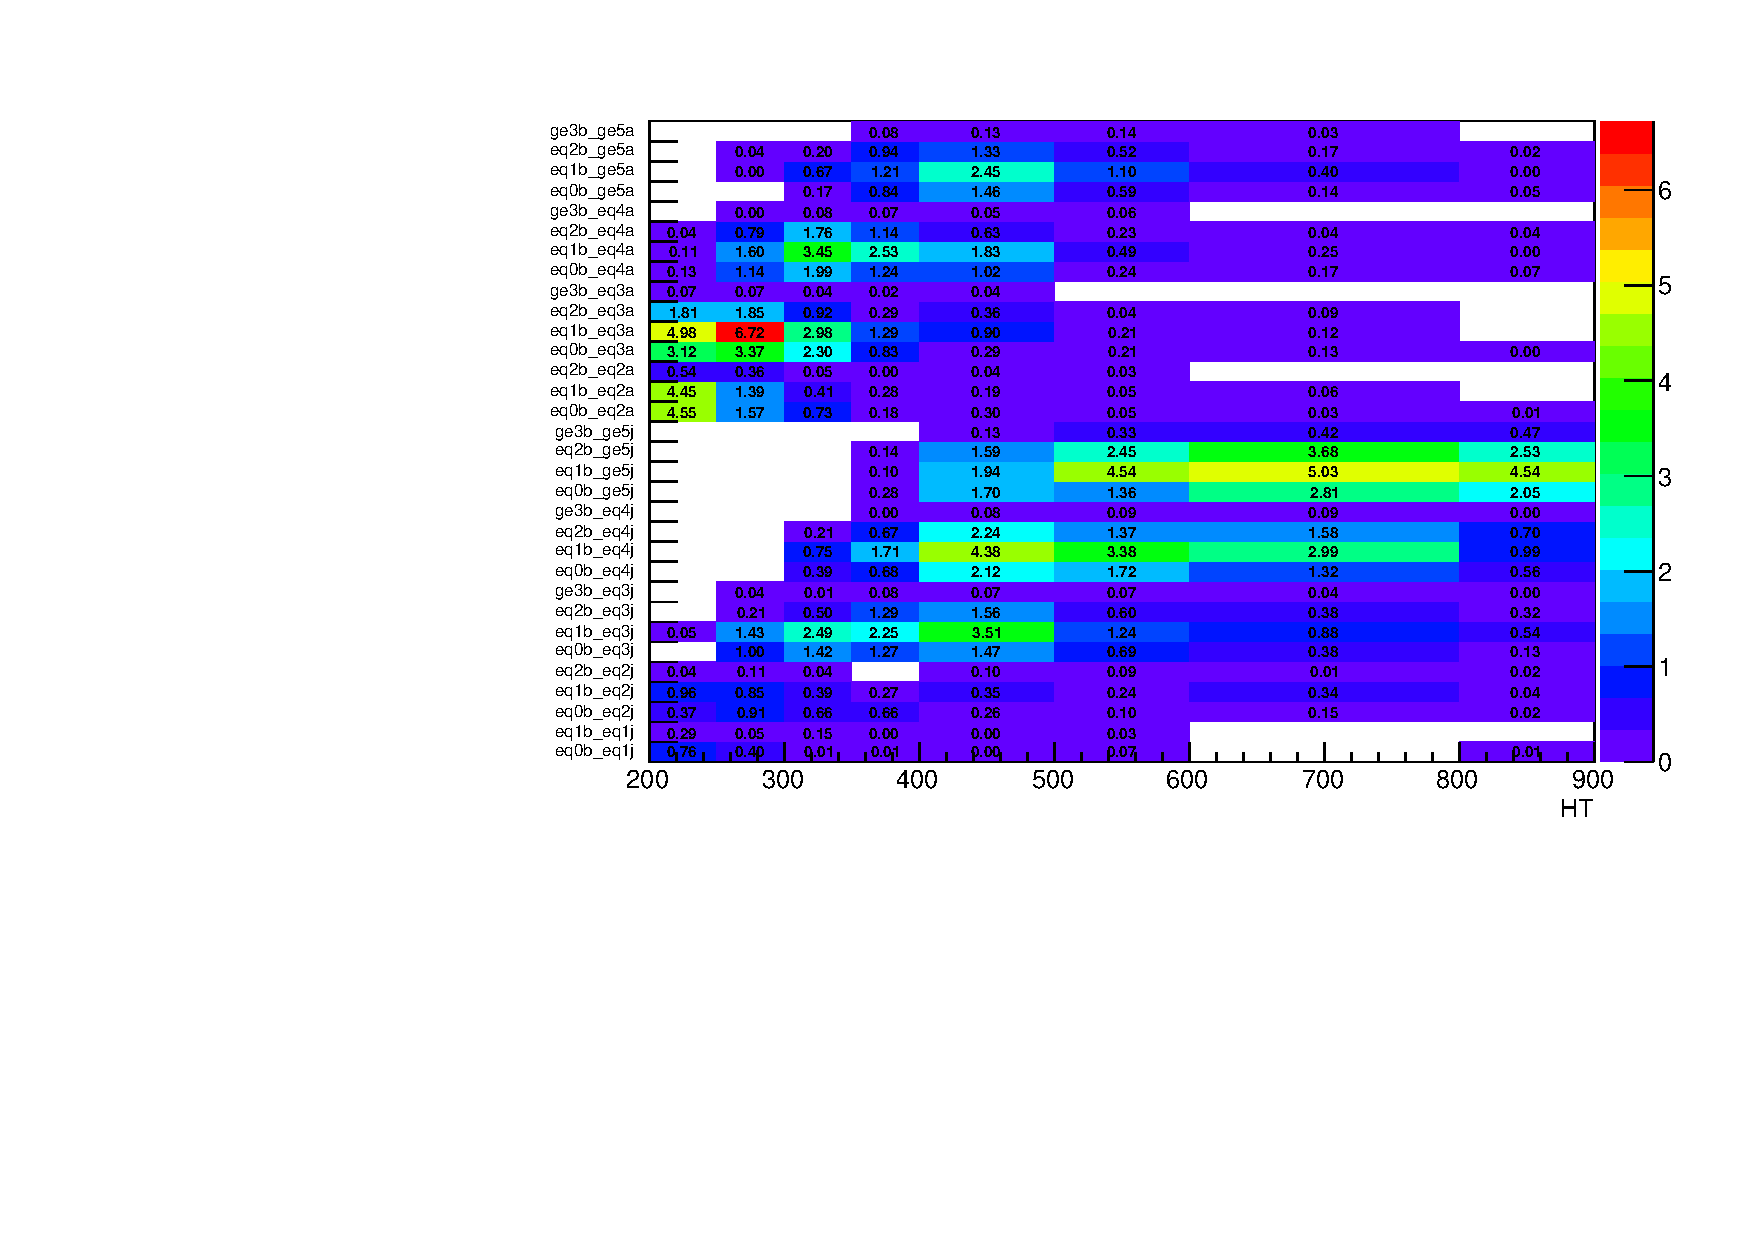
\includegraphics[width=0.5\textwidth]{figures/susyResults/sigYields_SingleMu_SMS-T2tt_mStop-250_mLSP-50_25ns}
%            \label{fig:contamination_T2tt_yields_mj}
%        } \\
%        \subfigure[Ratio of signal acceptance (\mj to signal region)]{
%            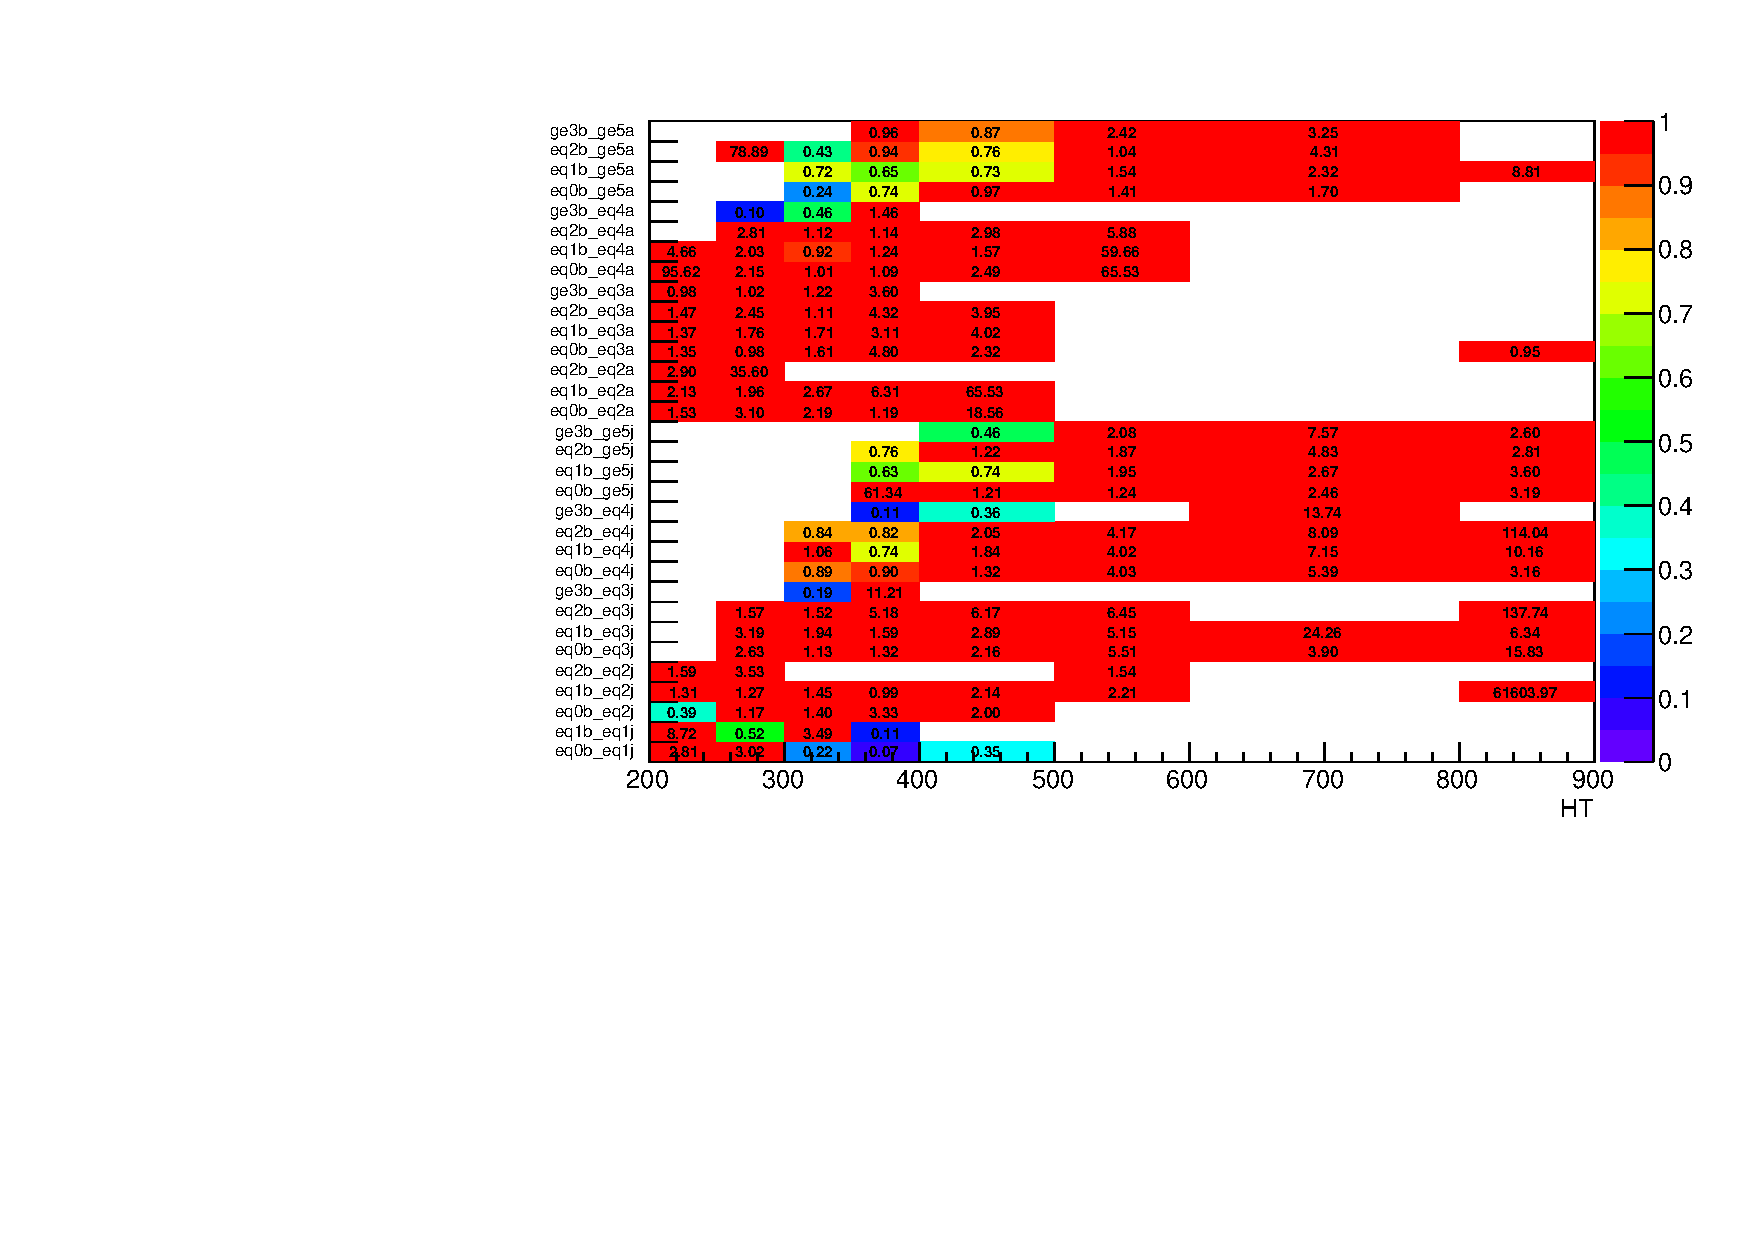
\includegraphics[width=0.5\textwidth]{figures/susyResults/relEff_SingleMu_SMS-T2tt_mStop-250_mLSP-50_25ns}
%            \label{fig:contamination_T2tt_relEff}
%        }
%        \subfigure[Ratio of S/B values (\mj to signal region)]{
%            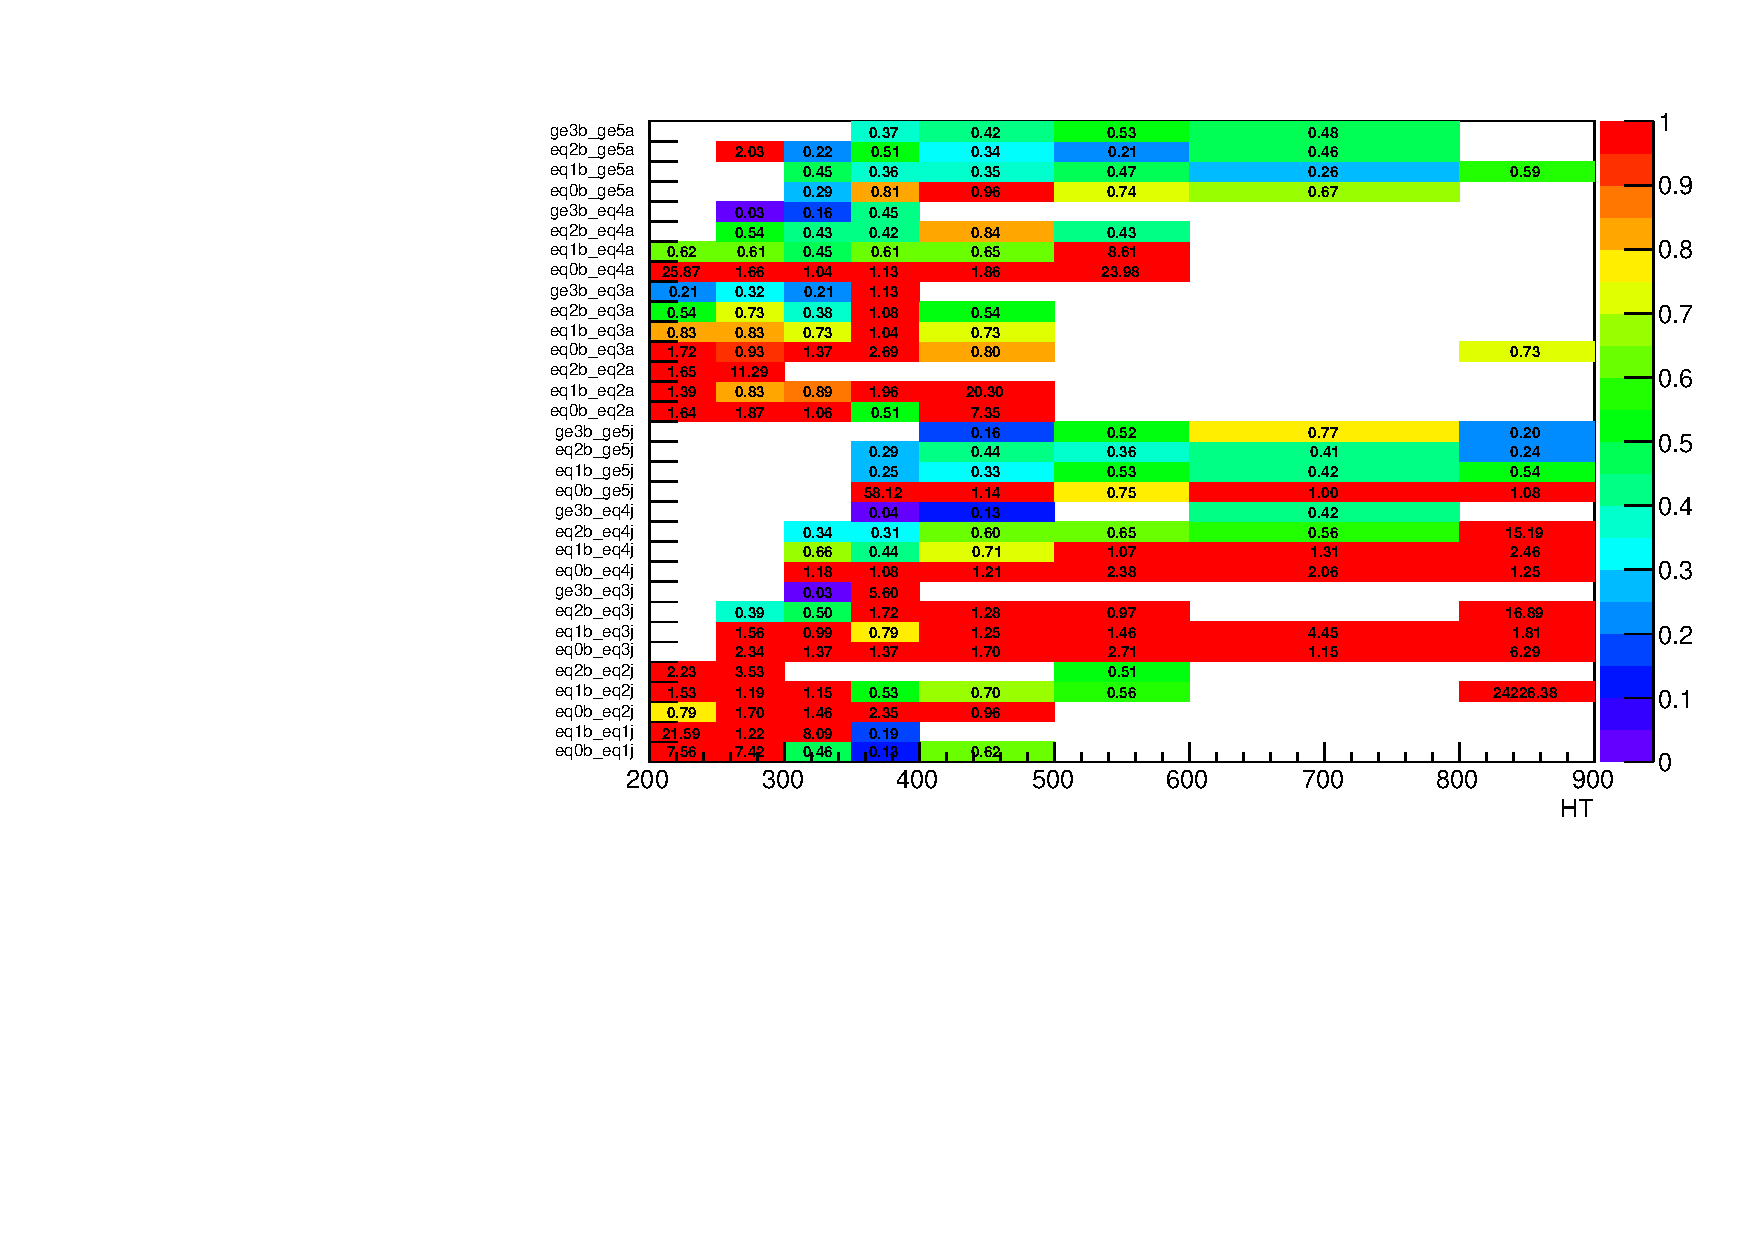
\includegraphics[width=0.5\textwidth]{figures/susyResults/doubleRatio_SingleMu_SMS-T2tt_mStop-250_mLSP-50_25ns}
%            \label{fig:contamination_T2tt_doubleRatio}
%        }
%        \caption{Characterisation of signal acceptance and contamination in the
%            signal and \mj control regions, respectively, for the benchmark
%            model T2tt (250,50).}
%        \label{fig:contamination_T2tt}
%    \end{center}
%\end{figure}

%The effect of signal contamination can be sizeable in these particular scenario
%for T2tt, as shown in Fig.~\ref{fig:contamination_T2tt_doubleRatio}, where in
%the most sensitive bins (high \nb, high \nj) the contribution of the control
%region sensitivity is comparable to the one of the signal region. However this
%is not an issue in the analysis, as the potential for signal contamination in
%all control samples is fully accounted for in the likelihood model used to
%extract the statistical interpretation (see Sec.~\ref{sec:likelihood}).
%
%The level of contamination for the \mmj sample is smaller still due to the
%requirement of a second muon.

\clearpage
\subsection{Systematic uncertainties on signal efficiency times acceptance}
\label{sec:sig-syst}

The following sources of systematic uncertainty are propagated to the signal
acceptance and shape, according to the recommendations agreed on within the
collaboration. Relative effect on the yields are presented in
Tab.~\ref{tab:sig-systematics} for some benchmark models.

\begin{itemize}
    \item Luminosity: 2.6\%, taken as correlated across all bins.
    \item Trigger: conservatively, the size of the inefficiency is taken as
        systematic variation where not in the plateau (see Sec.~\ref{sec:triggers}).
    \item MC statistics:  uncorrelated bin-by-bin uncertainty, affecting the
        shape of the signal.
    \item Pileup reweighting: 5.0\% uncertainty on the minimum bias cross section
        (see Sec.~\ref{sec:pileup-reweighting}).
    \item b-tag efficiency: uncertainty on the FullSim and FastSim b-tag scale
        factor is propagated and taken as correlated across the bins.
    \item Lepton efficiency: uncertainty on the lepton scale factors is
        propagated and taken as correlated across the bins.
    \item Jet energy scale: uncertainty on the jet energy corrections is
        propagated and taken as correlated across the bins.
    \item Initial State Radiation (ISR): Reweighting of the $N_{\text{isr}}$
        distribution. The systematic is taken as half the corrections.
\end{itemize}

\begin{table}[h!]
    \scriptsize
    \caption{
        Representative range taken from the $16\%$ and $84\%$ percentiles of the
        uncertainty across the analysis bins for each source of signal
        systematic. Two benchmark point are chosen for each model, corresponding
        to ``compressed'' and ``uncompressed'' scenarios, i.e. with small and
        large mass splitting between the mother particle and the LSP. A third
        benchmark is chosen for T2tt for the $W$ corridor and no
        ``uncompressed'' is chosen for T2cc.
    }
    \label{tab:sig-systematics}
    \centering
    \begin{tabular}{ ccccccccc }
        \hline \hline
        Model & ($m_{\mathrm{Susy}},m_{\mathrm{LSP}}$) & Luminosity & ISR & JEC & PU & b-tag & Trigger & MC stat. \\ \hline
        \multirow{2}{*}{T1qqqq}
            & (1700,100) & 2.6\% & 2-4\%  & 2-12\% & 6-12\% & 1-1\% & 1-2\% & 14-19\% \\
            & (1000,850) & 2.6\% & 3-14\% & 5-14\% & 9-14\% & 3-7\% & 2-4\% & 6-22\%  \\
        \hline
        \multirow{2}{*}{T1bbbb}
            & (1900,100)  & 2.6\% & 3-9\%  & 4-6\%  & 7-14\% & 7-12\% & 4-5\% & 11-19\% \\
            & (1300,1100) & 2.6\% & 2-11\% & 3-11\% & 5-9\%  & 2-5\%  & 1-3\% & 11-22\% \\
        \hline
        \multirow{2}{*}{T1tttt}
            & (1700,100) & 2.6\% & 2-6\% & 3-15\%  & 2-9\%  & 2-6\% & 2-4\% & 12-24\% \\
            & (950,600)  & 2.6\% & 5-9\% & 12-26\% & 7-13\% & 2-6\% & 3-7\% & 15-30\% \\
        \hline
        \multirow{2}{*}{T2qq (1-fold)}
            & (700,100) & 2.6\% & 2-7\%  & 3-10\% & 6-9\%  & 0-5\% & 1-4\% & 4-22\% \\
            & (400,300) & 2.6\% & 5-22\% & 5-18\% & 9-15\% & 3-5\% & 3-5\% & 6-20\% \\
        \hline
        \multirow{2}{*}{T2qq (8-fold)}
            & (1250,100) & 2.6\% & 2-7\%  & 5-14\% & 5-10\% & 1-1\% & 1-3\% & 12-24\% \\
            & (700,600)  & 2.6\% & 4-17\% & 4-13\% & 9-14\% & 2-5\% & 2-4\% & 6-22\%  \\
        \hline
        \multirow{2}{*}{T2bb}
            & (1000,100) & 2.6\% & 1-7\%  & 4-11\% & 5-9\%  & 1-4\% & 0-3\% & 14-23\% \\
            & (550,450)  & 2.6\% & 4-15\% & 4-15\% & 8-13\% & 3-7\% & 2-3\% & 9-22\%  \\ 
        \hline
        \multirow{2}{*}{T2tt}
            & (1000,50) & 2.6\% & 3-7\%   & 4-14\% & 6-10\%  & 1-5\%  & 1-4\%  & 14-27\% \\
            & (450,200) & 2.6\% & 4-12\%  & 6-15\% & 10-14\% & 4-9\%  & 3-6\%  & 6-19\%  \\
            & (250,150) & 2.6\% & 13-27\% & 8-22\% & 12-25\% & 6-16\% & 6-17\% & 10-23\% \\
        \hline
        \multirow{1}{*}{T2cc}
            & (500,480) & 2.6\% & 4-18\% & 5-13\% & 5-12\% & 1-4\% & 2-4\% & 6-19\% \\
        \hline \hline
    \end{tabular}
\end{table}

\clearpage
\subsection{Exclusion limits and significance}
\label{sec:susy_results}

In order to extract the signal contribution in the fit, the
distribution of events according to the \mht variable, encoded as
template histograms as described in
Secs.~\ref{sec:htmiss-categorisation}, \ref{sec:mht-intro},
\ref{sec:mht-zinv-intro}, and \ref{sec:likelihood}, is used.

Upper limits on the cross section are computed using the
$\text{CL}_{s}$ criterion \cite{CLsTechnique}. Asymptotic formulae
\cite{AsymptoticFormulae} are
utilised to approximate the distribution of the test statistics. 

All the statistical results are produced using the \textit{combine}
tool, provided within the HiggsAnalysis-CombinedLimit package
\cite{Combine}.

In Figs.~\ref{fig:T1qqqq}-\ref{fig:T2cc} (top) the 95\% C.L. upper
limits on the cross section are shown in the
$(m_{\mathrm{Susy}},m_{\mathrm{LSP}})$ plane for the models considered
in this interpretation. These results correspond to 35.9~\ifb of
integrated luminosity. The exclusion contour is also shown together
with $\pm1\sigma$ (and $\pm2\sigma$ for the expected exclusion)
uncertainty.  The band around the expected exclusion reflects the
experimental uncertainty, while the band around the observed exclusion
correspond to the theoretical uncertainty on the signal cross section.

In Figs.~\ref{fig:T1qqqq}-\ref{fig:T2cc} (left) the signal
acceptance for each mass point in the SMS scan.

In Figs.~\ref{fig:T1qqqq}-\ref{fig:T2cc} (right) each mass point
is assigned a group of 4 jet categories in descending order of
sensitivity. The total number of mass points with the same 4 most
sensitive jet categories is noted. In the gluino production models in the
uncompressed regions the high jet multiplicities drive the sensitivity (ge6j,
eq5j, eq4j), and in the compressed regions the same high jet multiplicities
drive the sensitivity with the asymmetric jet topologies playing a larger role
than in the uncompressed regions. In the T2qq and T2bb models, the sensitivity
in the uncompressed regions are driven by low/medium jet multiplicities (eq2j,
eq3j, eq4j), and in the compressed regions it's driven by high jet
multiplicities (ge6j, eq5j, eq4j). In stop production models the uncompressed
and compressed regions are driven by high jet multiplicities (ge6j, eq5j, eq4j)
with the asymmetric topology playing a larger role in the compressed regions.
The weakest jet multiplicity, in terms of limit sensitivity, is the monojet
category and is expected to become sensitive for Dark matter models.

In Figs.~\ref{fig:T1qqqq}-\ref{fig:T2cc} (bottom) the local observed
significance for each mass point in the SMS scan is shown.

The models are grouped according to the following categorisation:
\begin{itemize}
    \item \textbf{Gluino-mediated production of off-shell (decoupled) 3rd generation squarks}:
        gluino pair production followed by 3-body decay to $t\bar{t}\chiz$,$b\bar{b}\chiz$.
        It includes T1bbbb and T1tttt.
    \item \textbf{Direct and gluino-mediated production of off-shell (decoupled) light-flavour squarks}:
        gluino/light squark pair production followed by 3-body/2-body decay to
        $q(q)\chiz$. It includes T1qqqq and T2qq.
    \item \textbf{Direct production of 3rd generation squarks}: stop/sbottom
        pair production, with several possibility for the decay
        (see Tab.~\ref{tab:simplified-models}). It includes T2bb, T2tt and T2cc.
\end{itemize}

%Summary exclusion plots according to this categorisation are presented in
%Fig.~\ref{fig:summary-excl-plots}.

\newpage
\begin{figure}[h!]
    \begin{center}
        \subfigure[T1qqqq: Upper limit on the cross section in the mass plane]{
            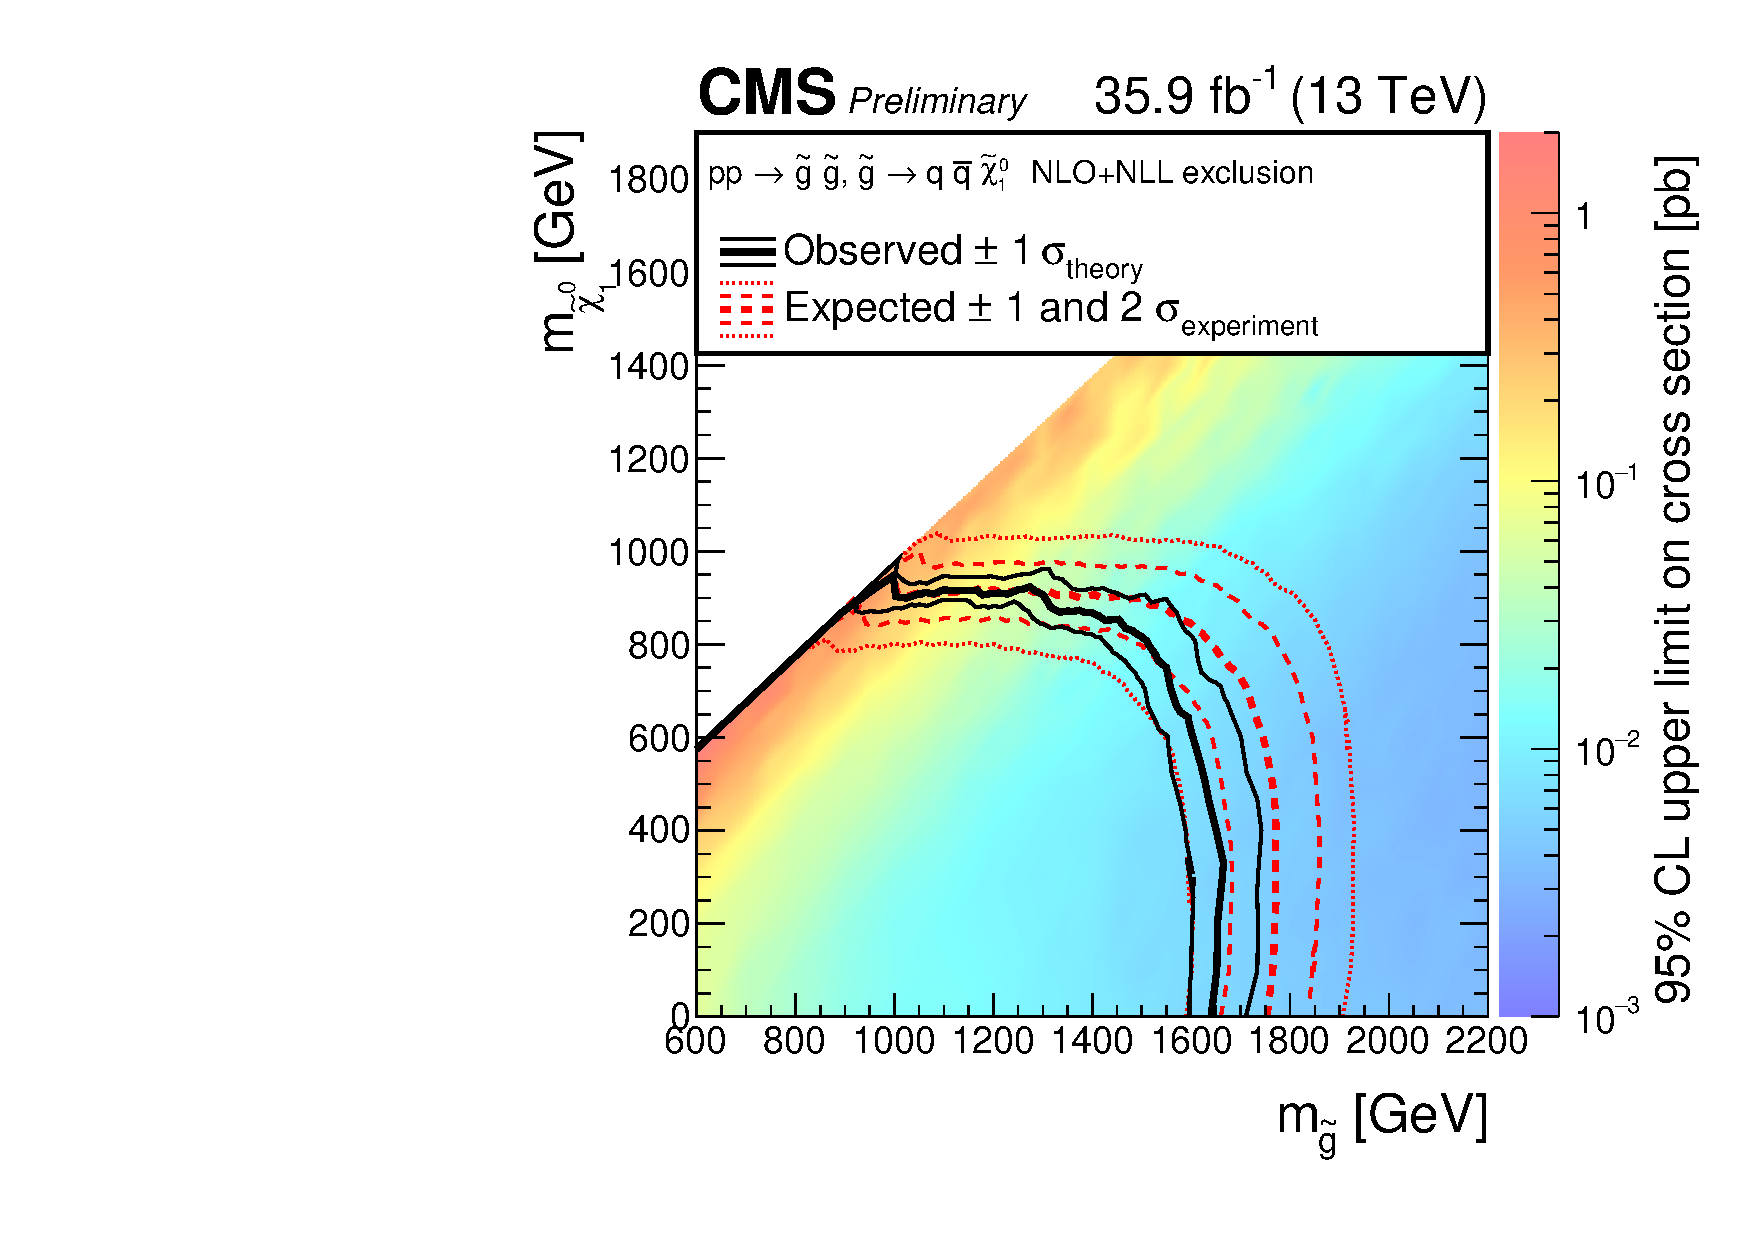
\includegraphics[width=0.6\textwidth]{figures/susyResults/T1qqqqXSEC}
            \label{fig:T1qqqq_excl}
        } \\
        \subfigure[T1qqqq: $\epsilon_{sig}$]{
            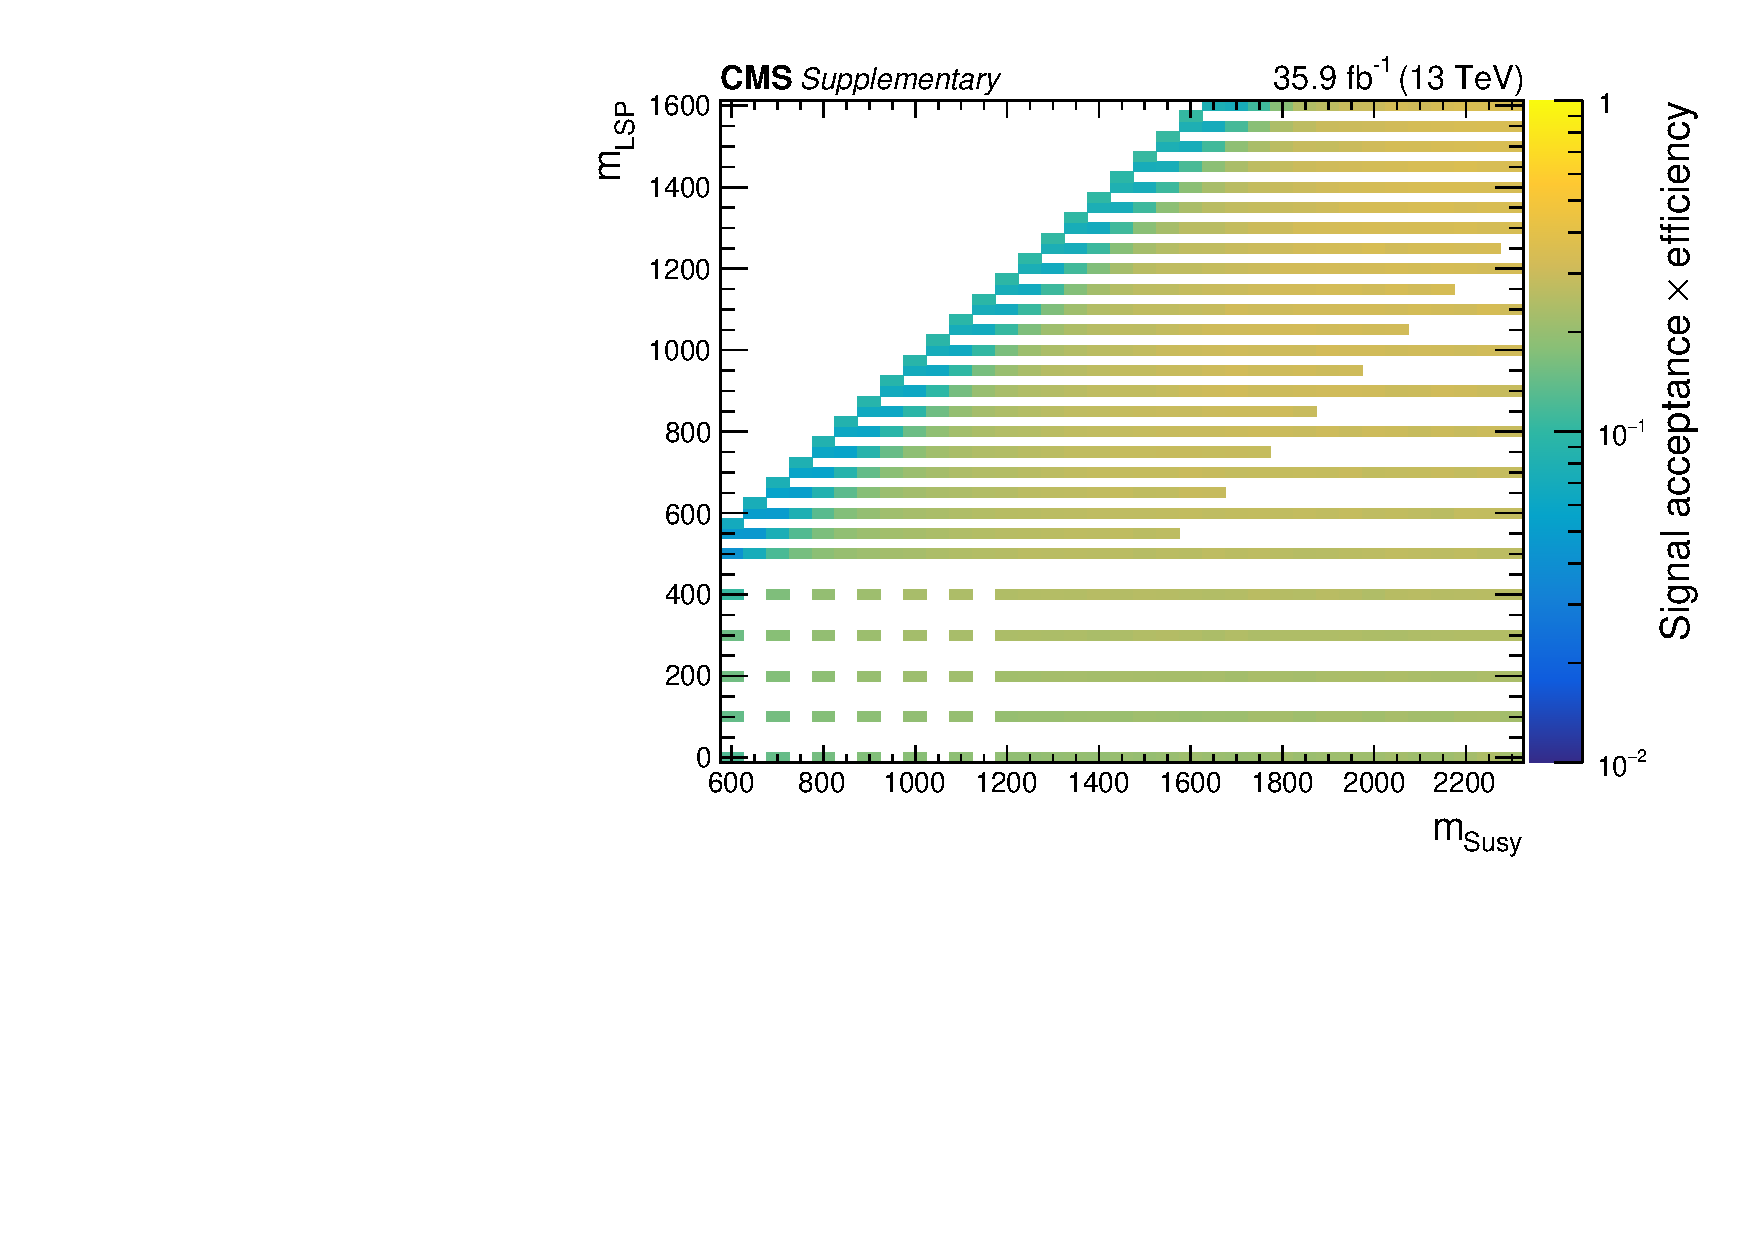
\includegraphics[width=0.45\textwidth]{figures/susyResults/T1qqqq_effs}
            \label{fig:T1qqqq_eff}
        } ~~
        \subfigure[T1qqqq: Most sensitive categories]{
            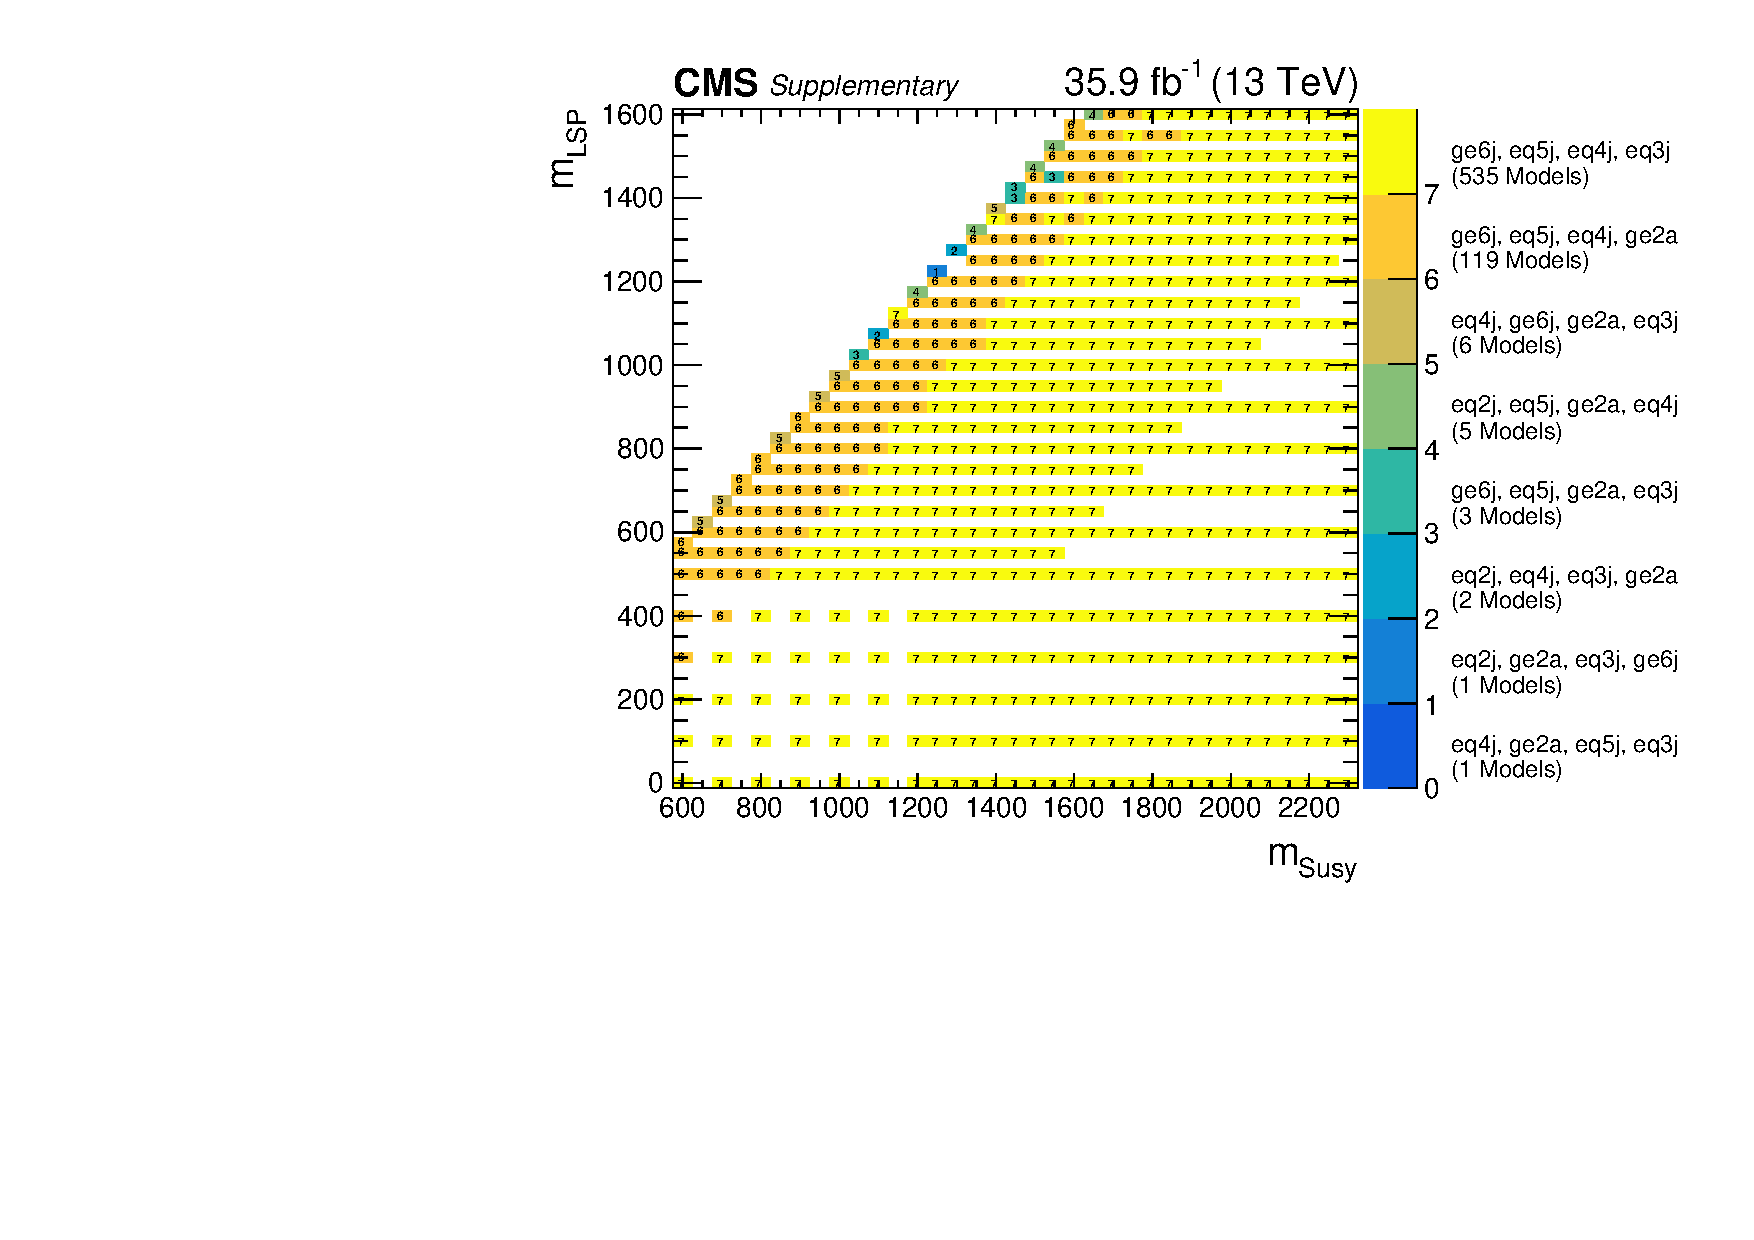
\includegraphics[width=0.45\textwidth]{figures/susyResults/T1qqqq_bitMap}
            \label{fig:T1qqqq_bitMap}
        } \\
        %\subfigure[T1qqqq: Significance scan]{
        %    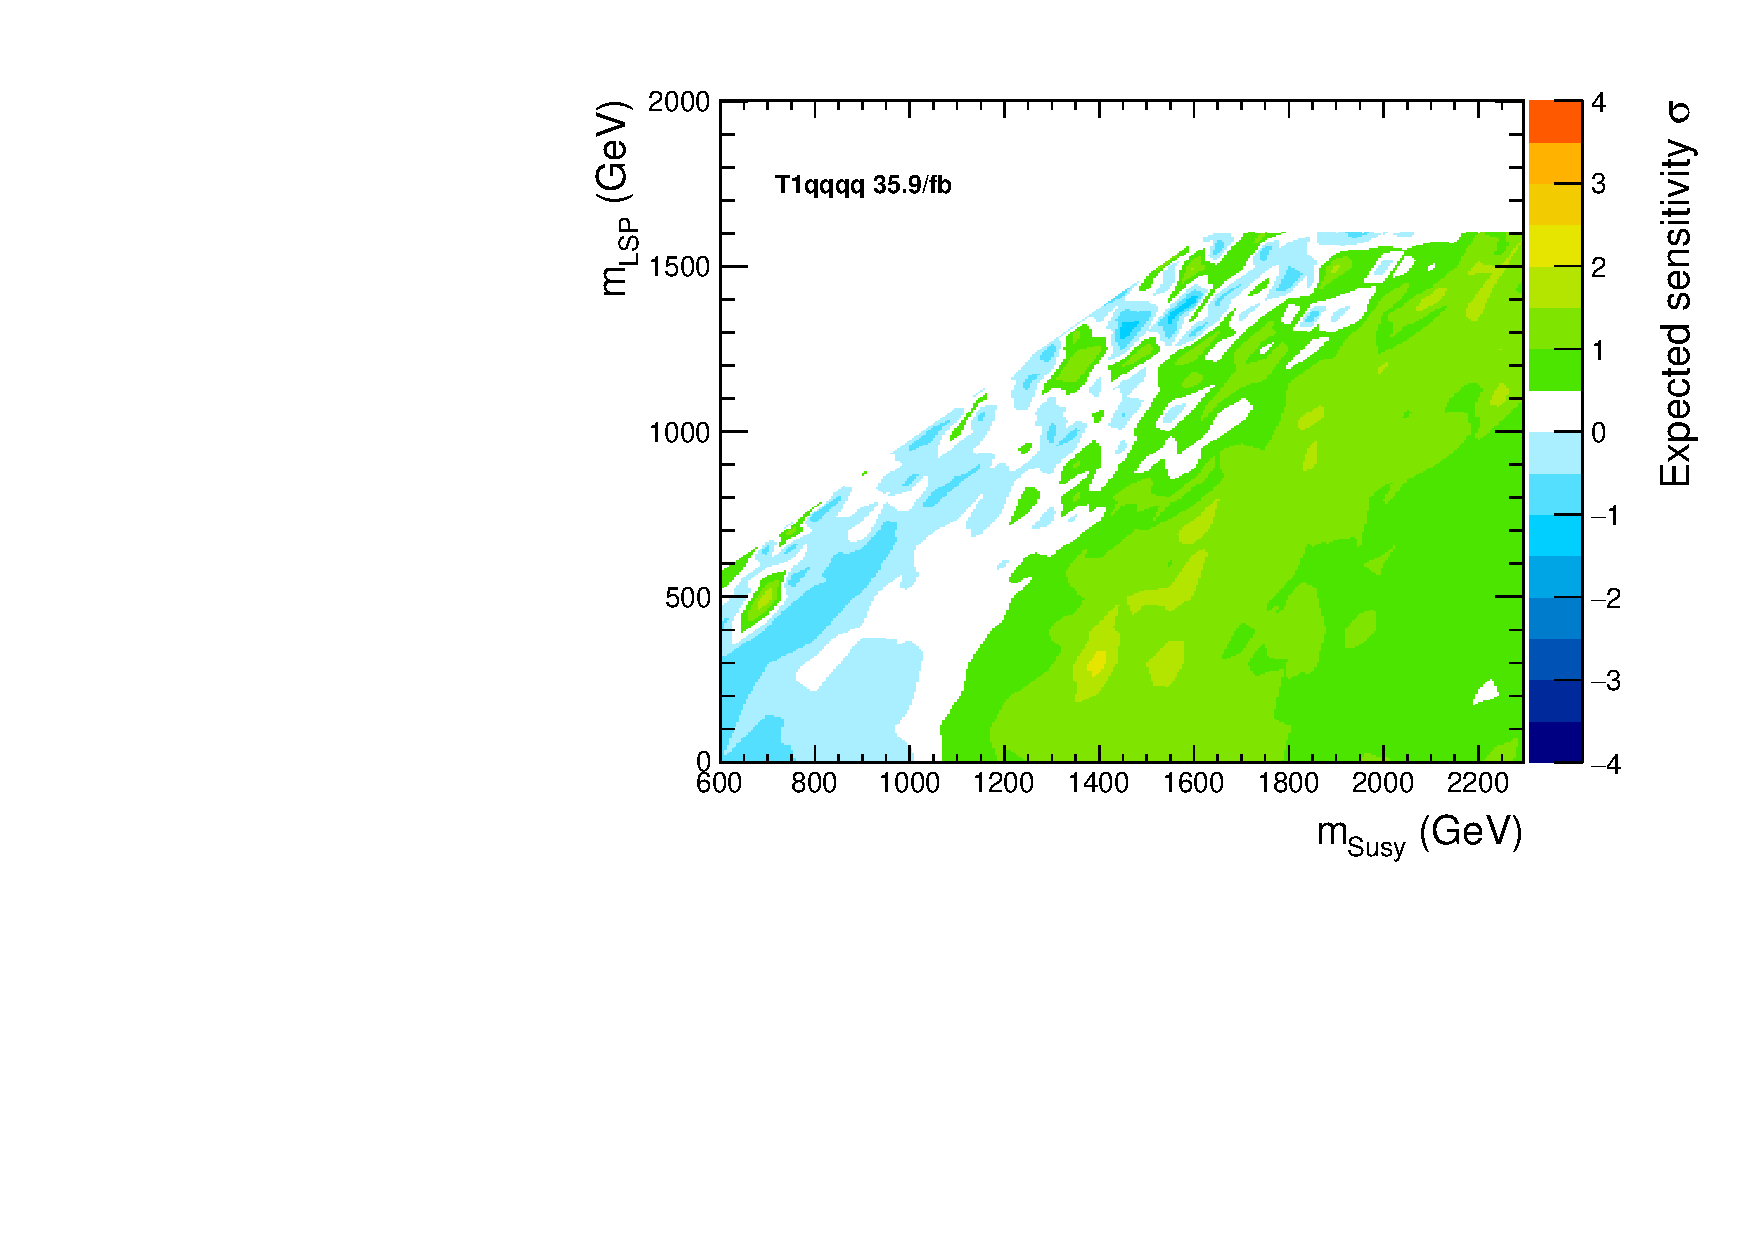
\includegraphics[width=0.45\linewidth]{figures/susyResults/T1qqqq_signif}
        %    \label{fig:T1qqqq_signif}
        %} ~~
        \caption{Top: the 95\% C.L. observed upper limit on the cross section
            (histogram), with the expected (solid black line) observed
            (solid red line) exclusion contours. Left: signal acceptance
            including all jet categories. Right: graph showing the four
            most sensitive jet categories for each mass point. Bottom:
            local observed significance scan.
        }
        \label{fig:T1qqqq}
    \end{center}
\end{figure}

\newpage
\begin{figure}[h!]
    \begin{center}
        \subfigure[T1bbbb: Upper limit on the cross section in the mass plane]{
            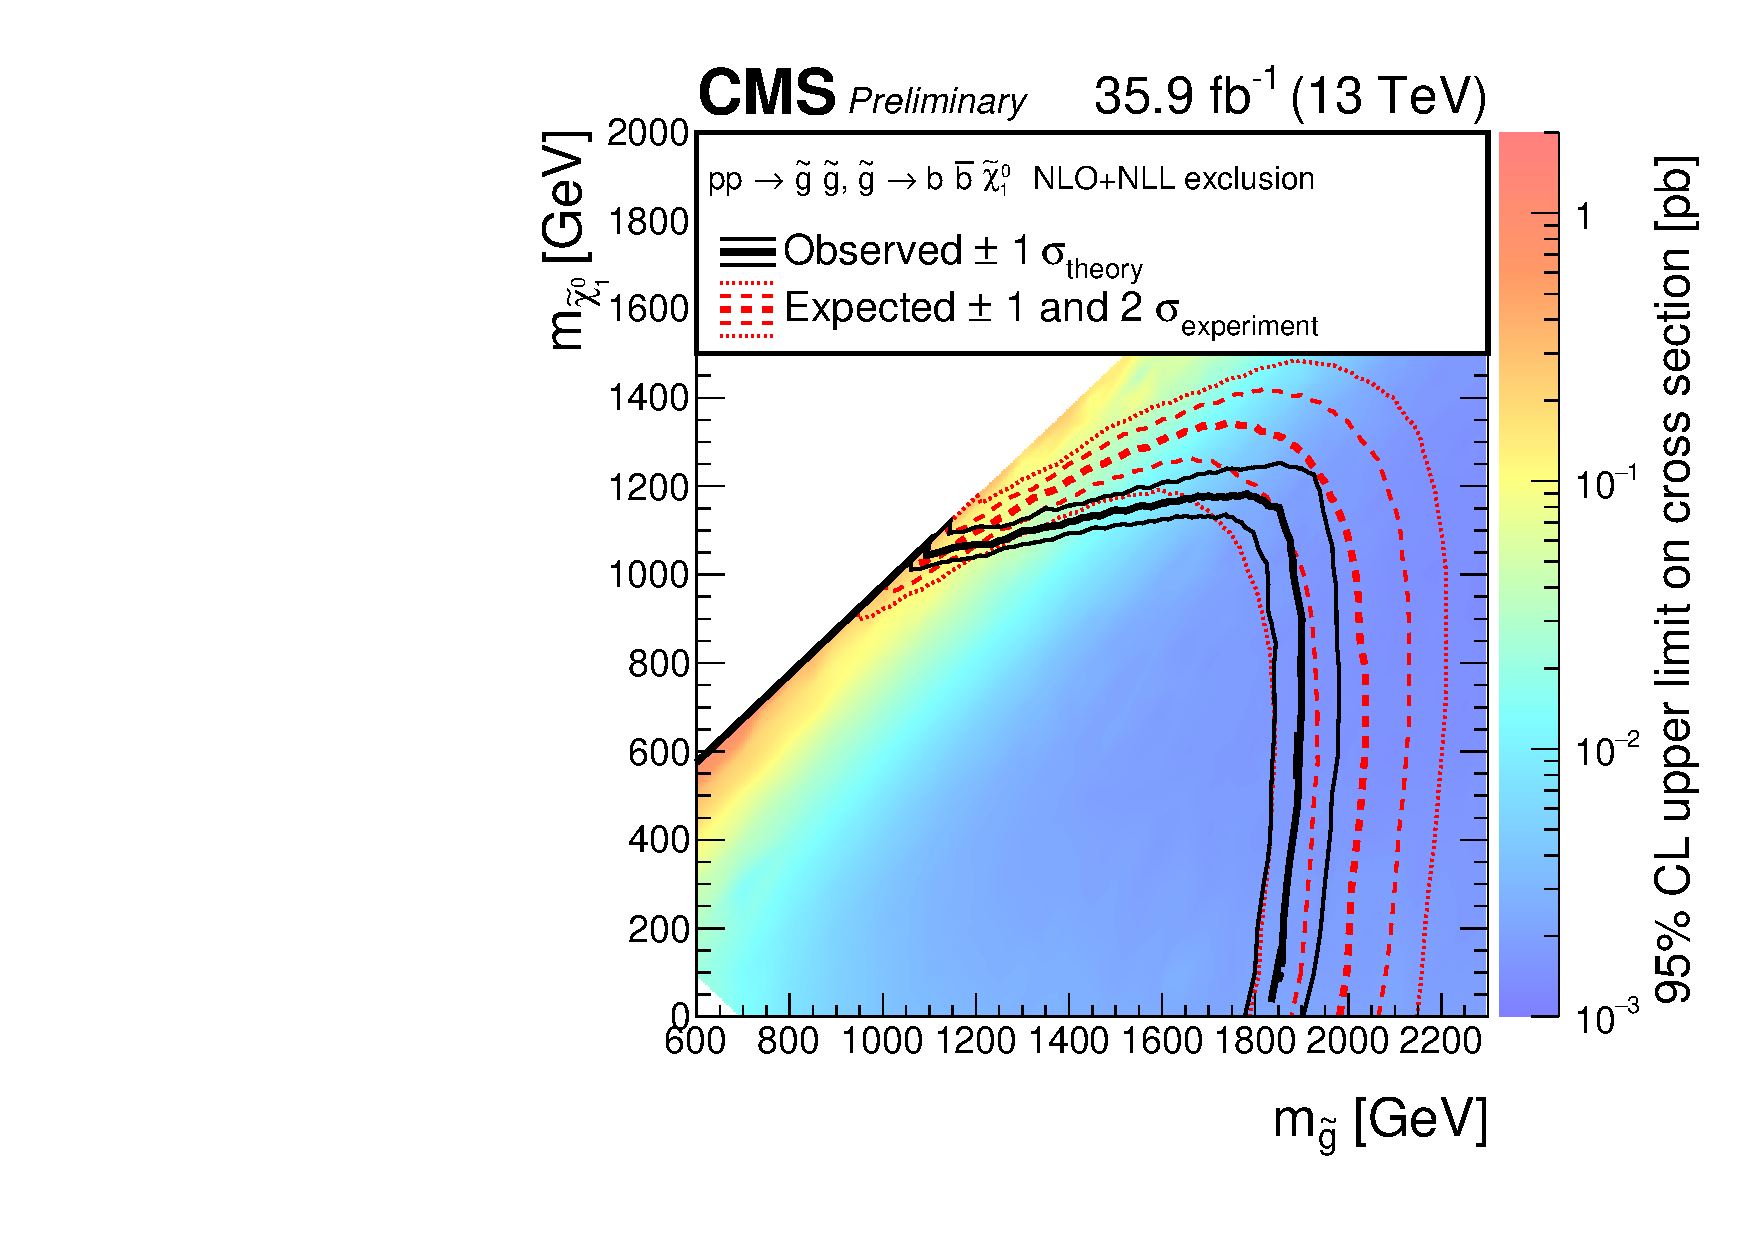
\includegraphics[width=0.6\textwidth]{figures/susyResults/T1bbbbXSEC}
            \label{fig:T1bbbb_excl}
        } \\
        \subfigure[T1bbbb: $\epsilon_{sig}$]{
            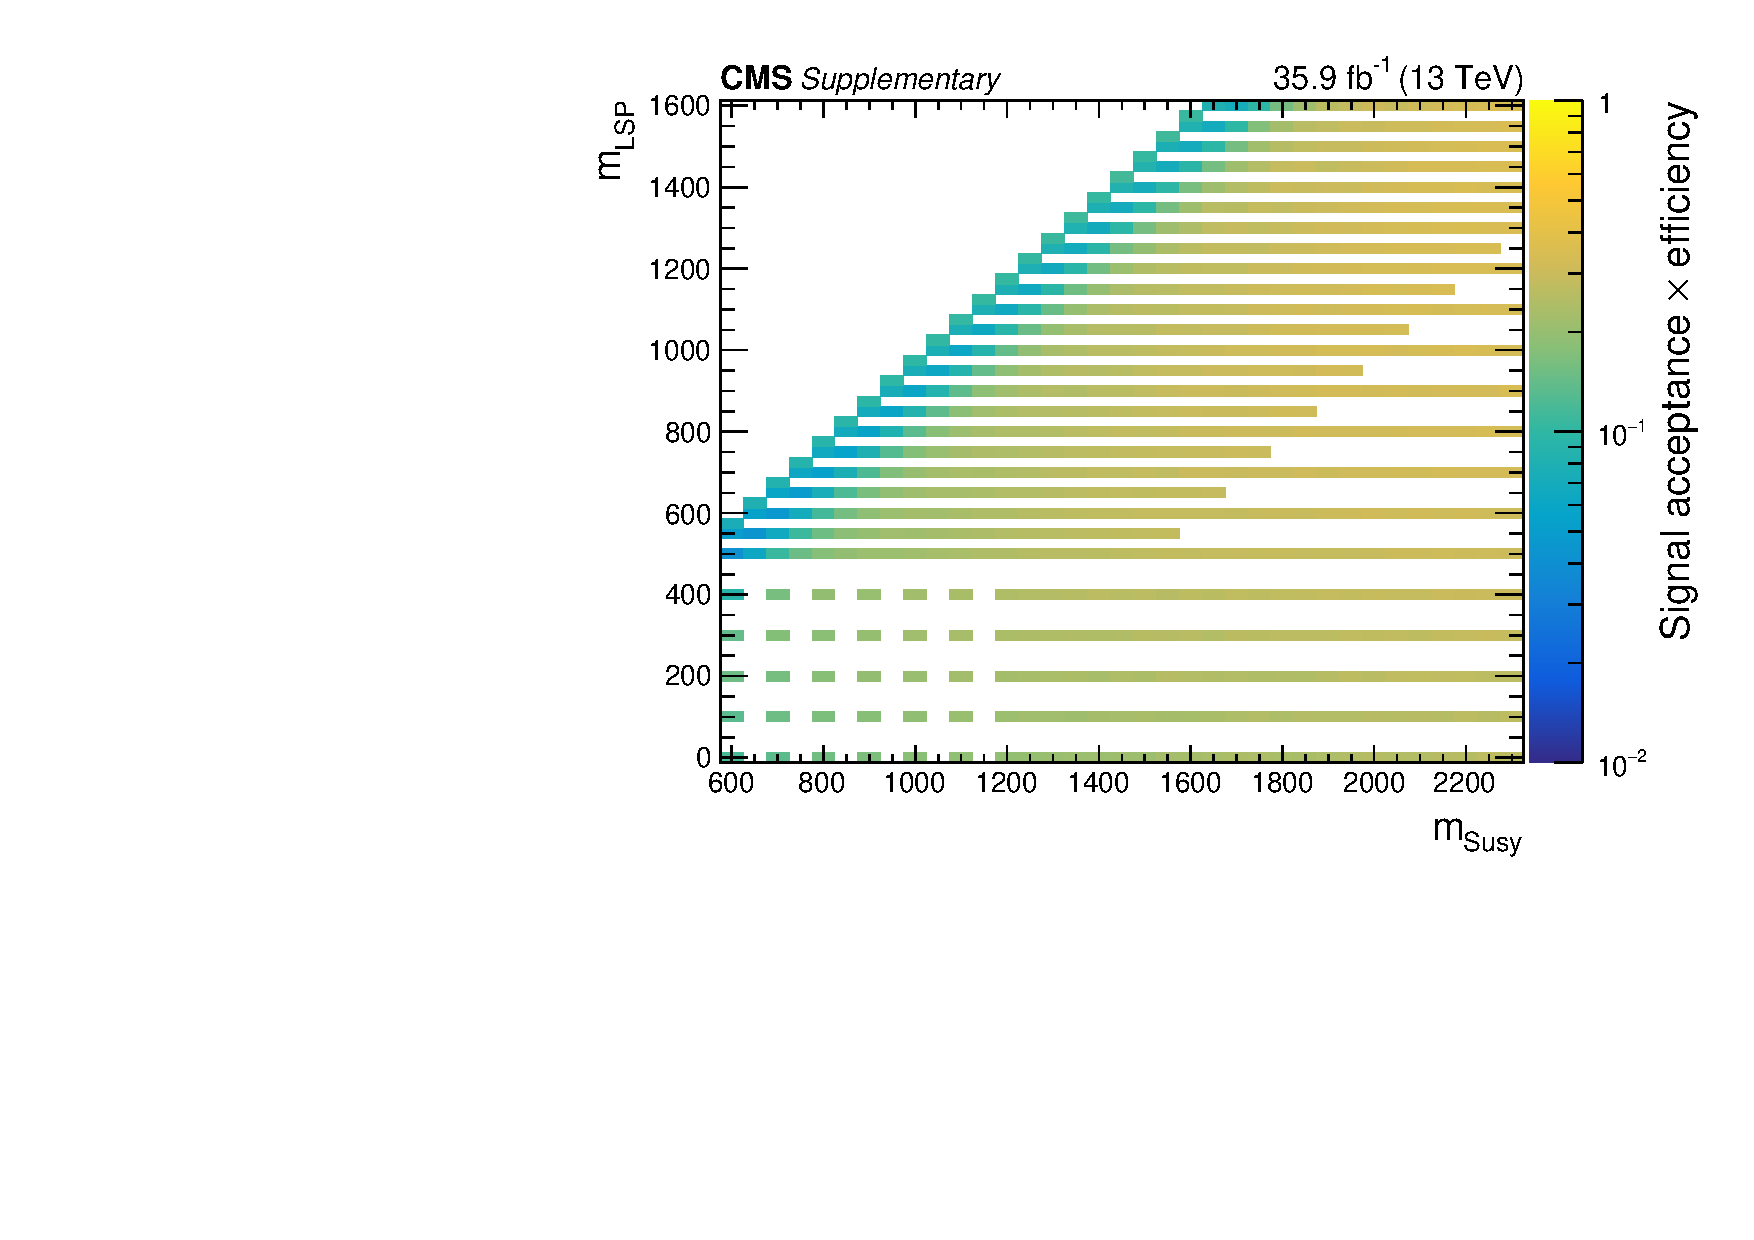
\includegraphics[width=0.45\textwidth]{figures/susyResults/T1bbbb_effs}
            \label{fig:T1bbbb_eff}
        } ~~
        \subfigure[T1bbbb: Most sensitive categories]{
            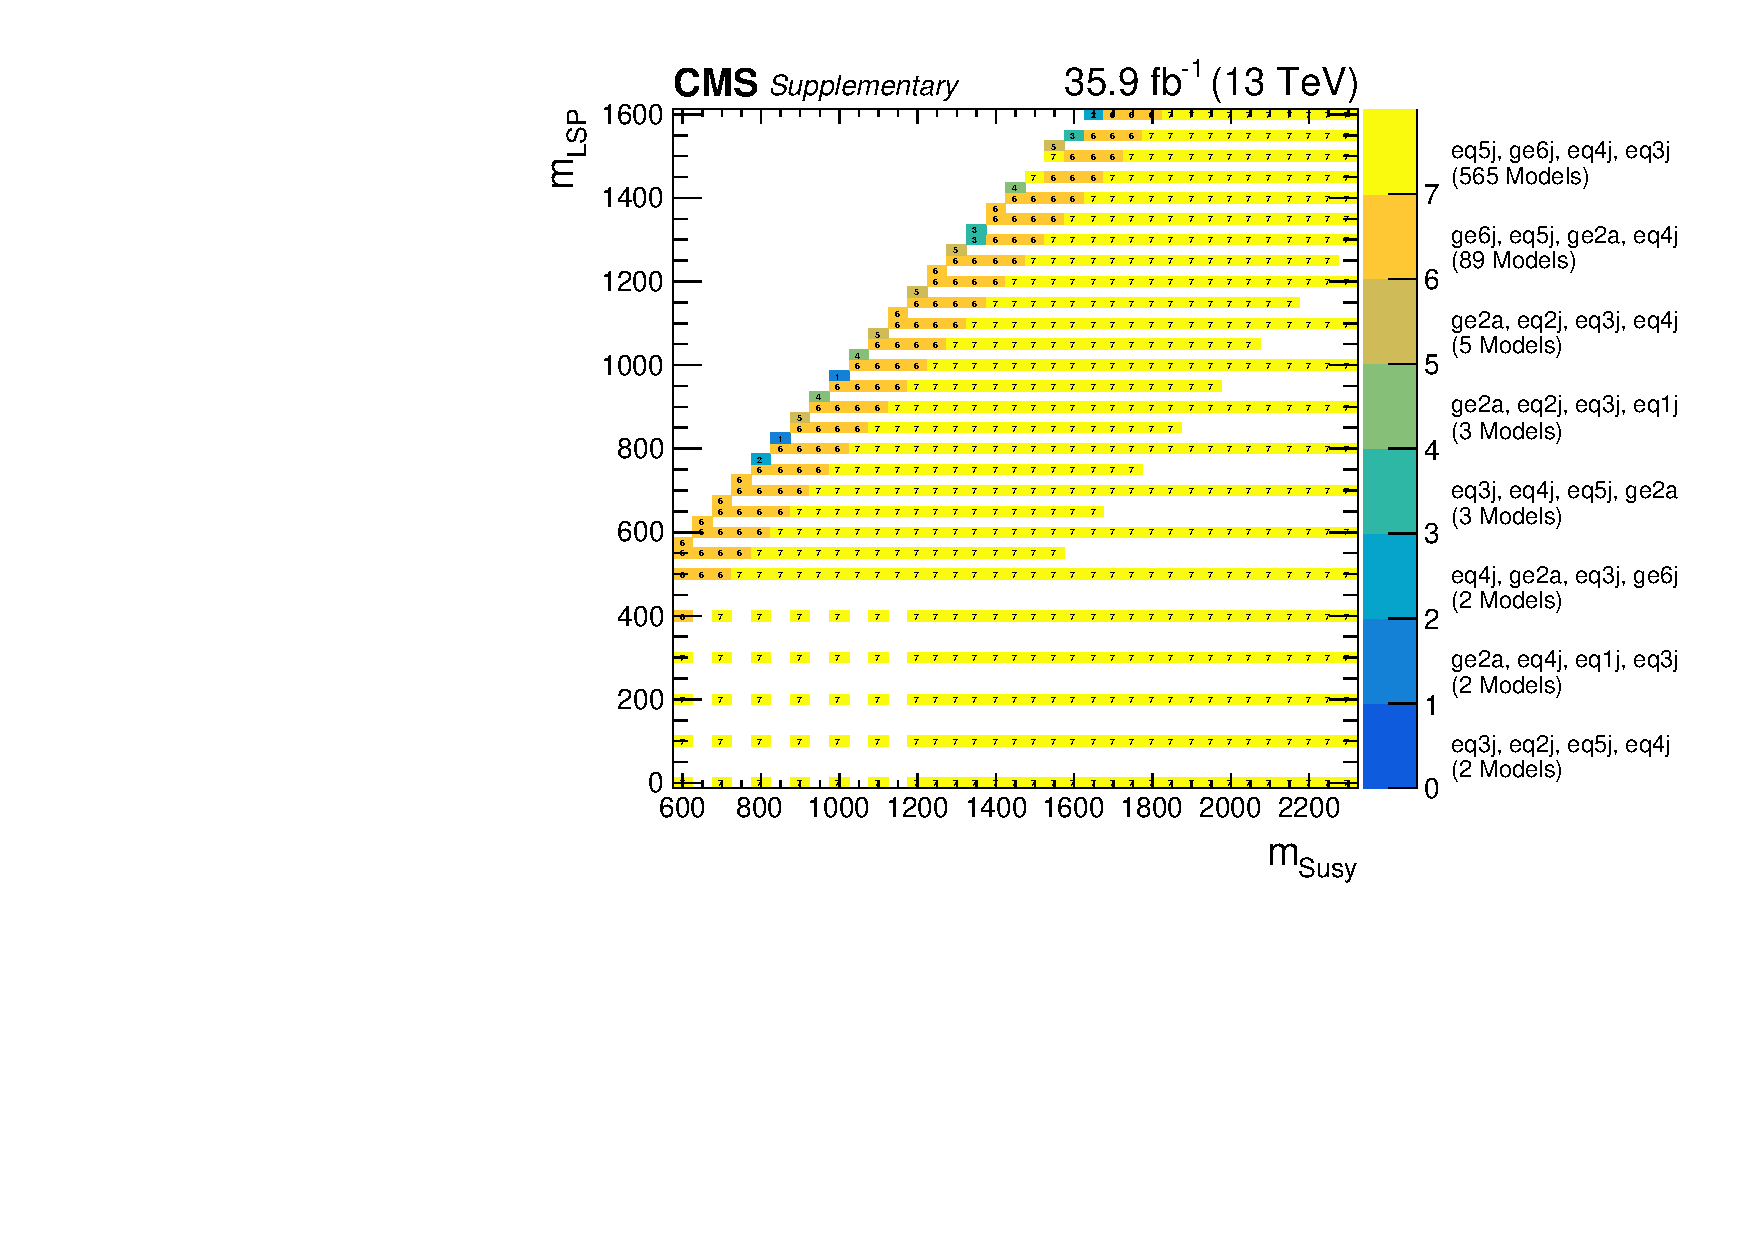
\includegraphics[width=0.45\textwidth]{figures/susyResults/T1bbbb_bitMap}
            \label{fig:T1bbbb_bitMap}
        } \\
        \subfigure[T1bbbb: Significance scan]{
            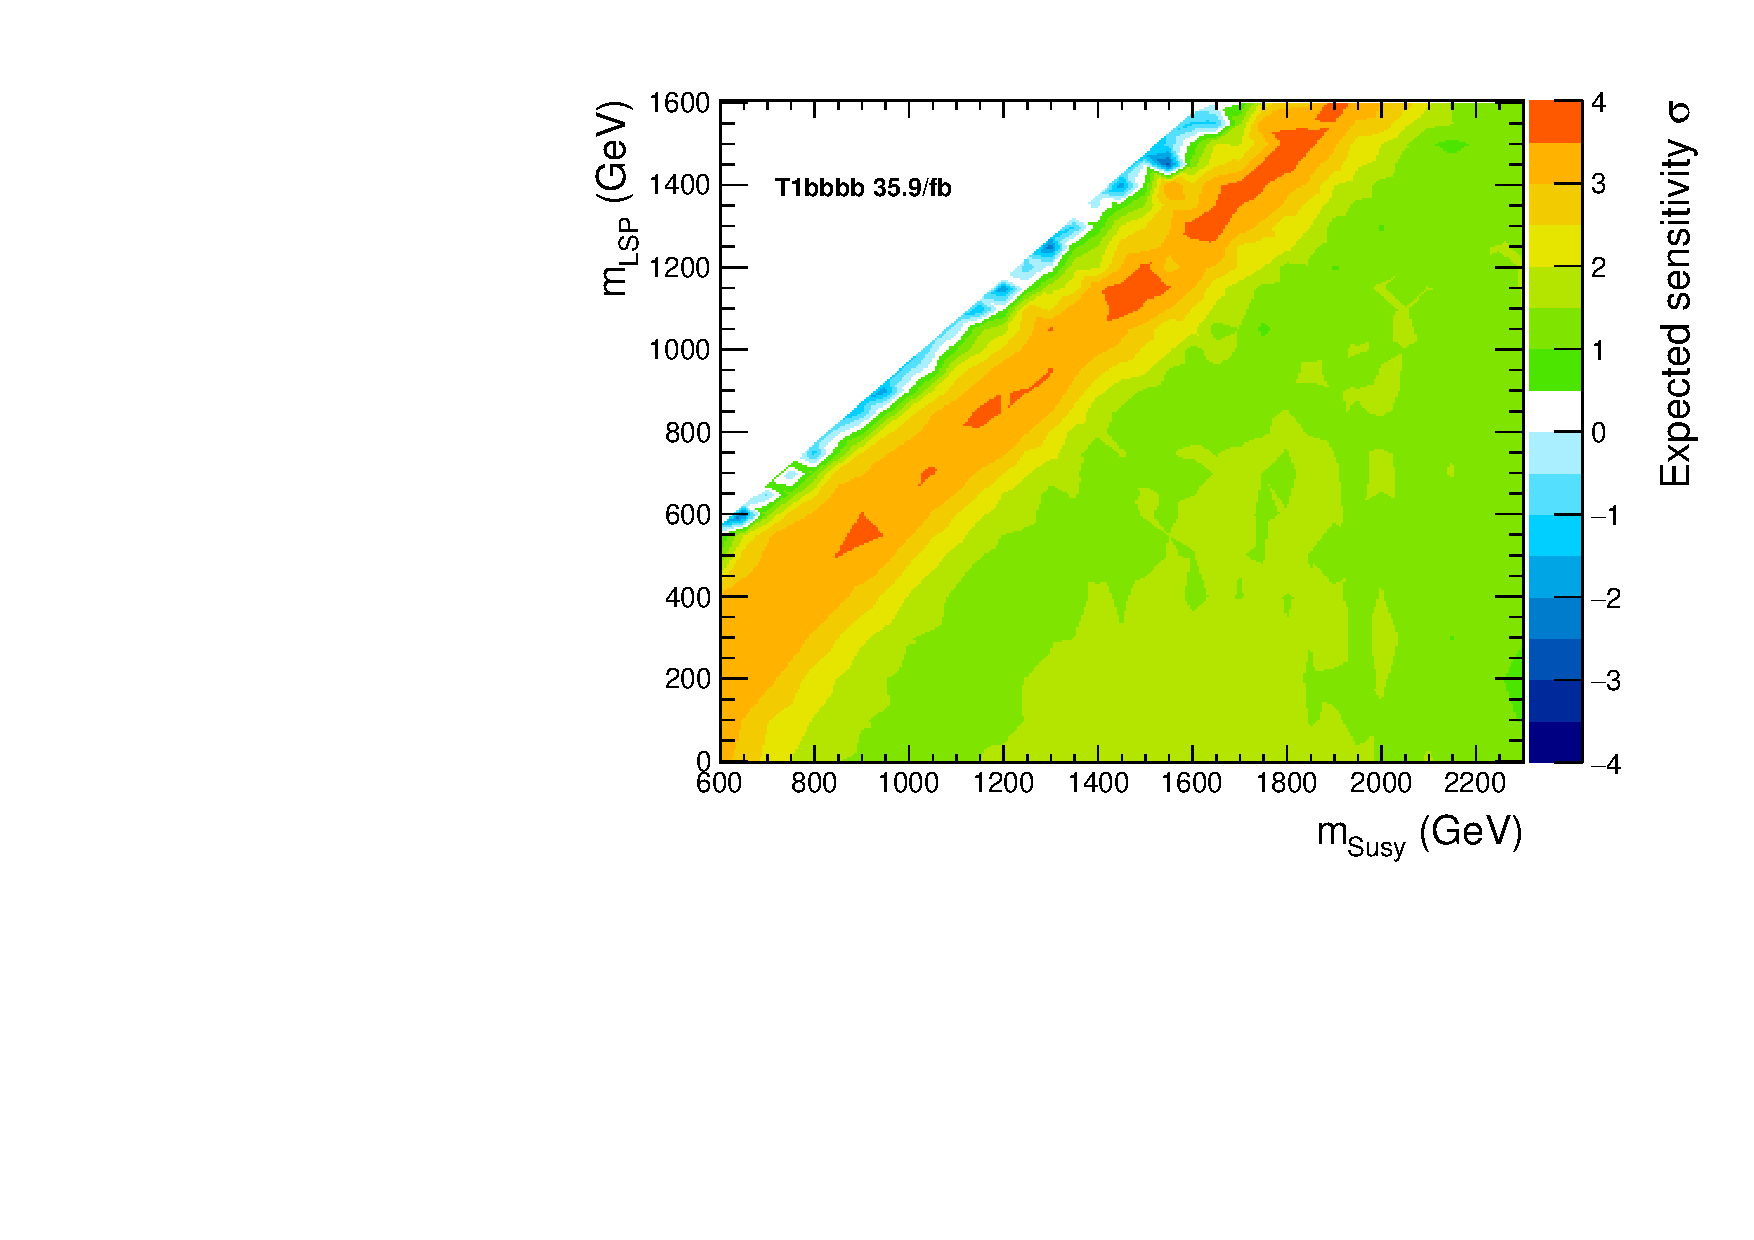
\includegraphics[width=0.45\linewidth]{figures/susyResults/T1bbbb_signif}
            \label{fig:T1bbbb_signif}
        } ~~
        \caption{Top: the 95\% C.L. observed upper limit on the cross section
            (histogram), with the expected (solid black line) observed
            (solid red line) exclusion contours. Left: signal acceptance
            including all jet categories. Right: graph showing the four
            most sensitive jet categories for each mass point. Bottom:
            local observed significance scan.
        }
        \label{fig:T1bbbb}
    \end{center}
\end{figure}

\newpage
\begin{figure}[h!]
    \begin{center}
        \subfigure[T1tttt: Upper limit on the cross section in the mass plane]{
            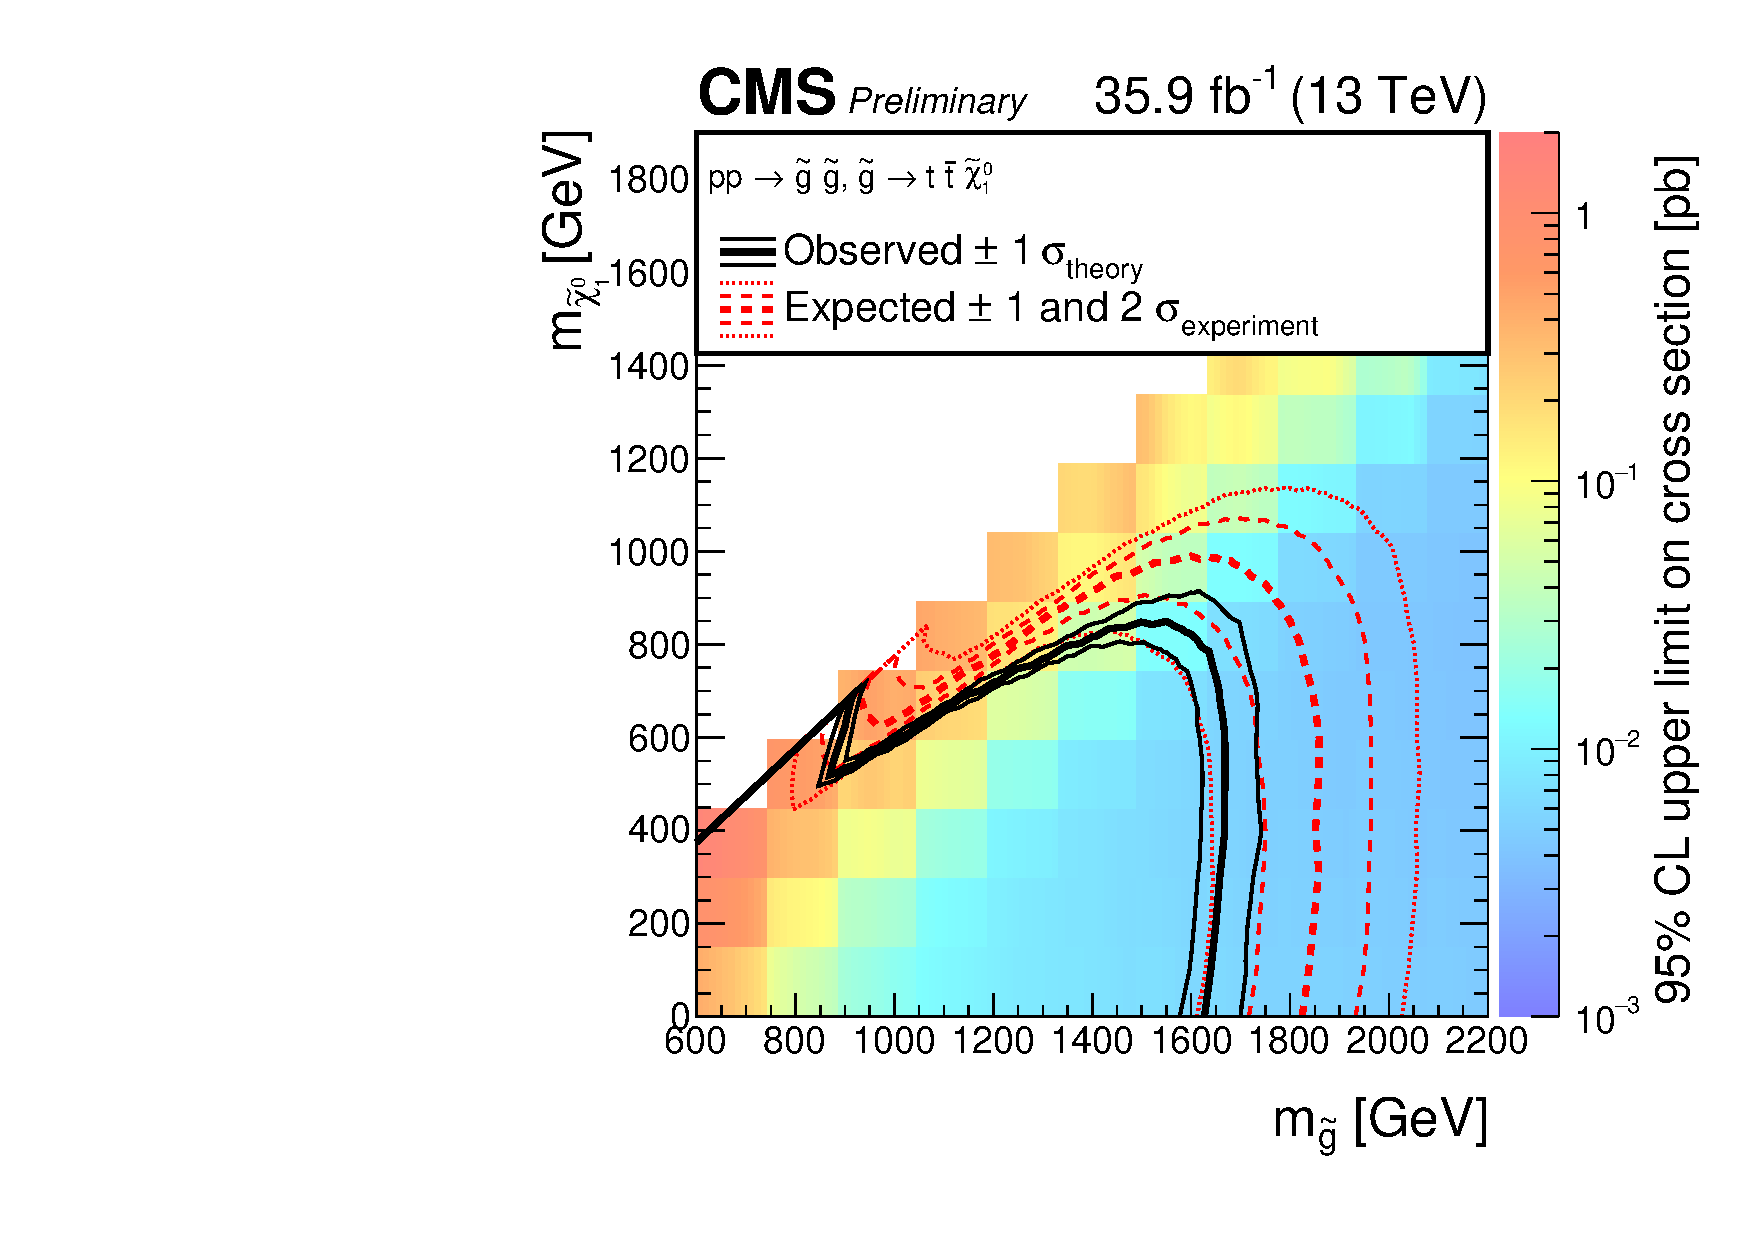
\includegraphics[width=0.6\textwidth]{figures/susyResults/T1ttttXSEC}
            \label{fig:T1tttt_excl}
        } \\
        \subfigure[T1tttt: $\epsilon_{sig}$]{
            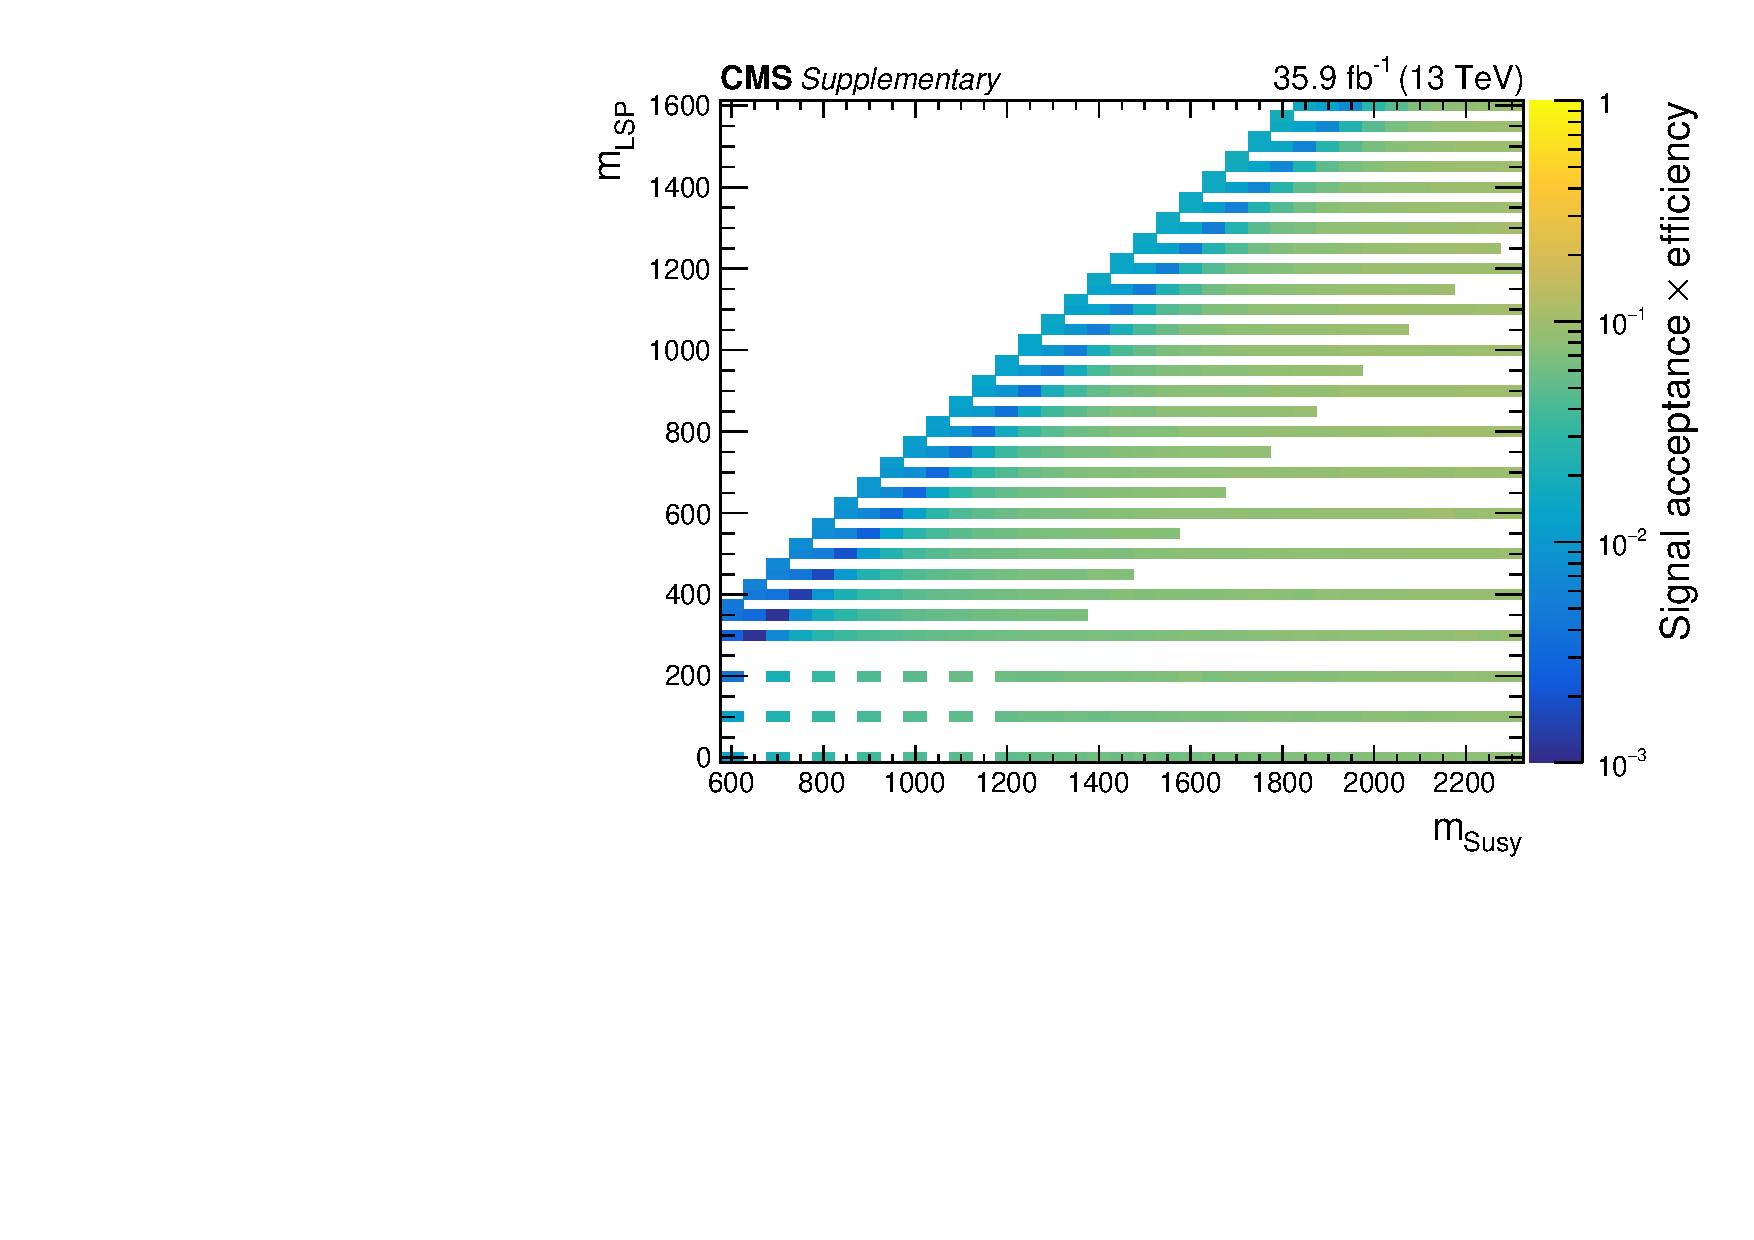
\includegraphics[width=0.45\textwidth]{figures/susyResults/T1tttt_effs}
            \label{fig:T1tttt_eff}
        } ~~
        \subfigure[T1tttt: Most sensitive categories]{
            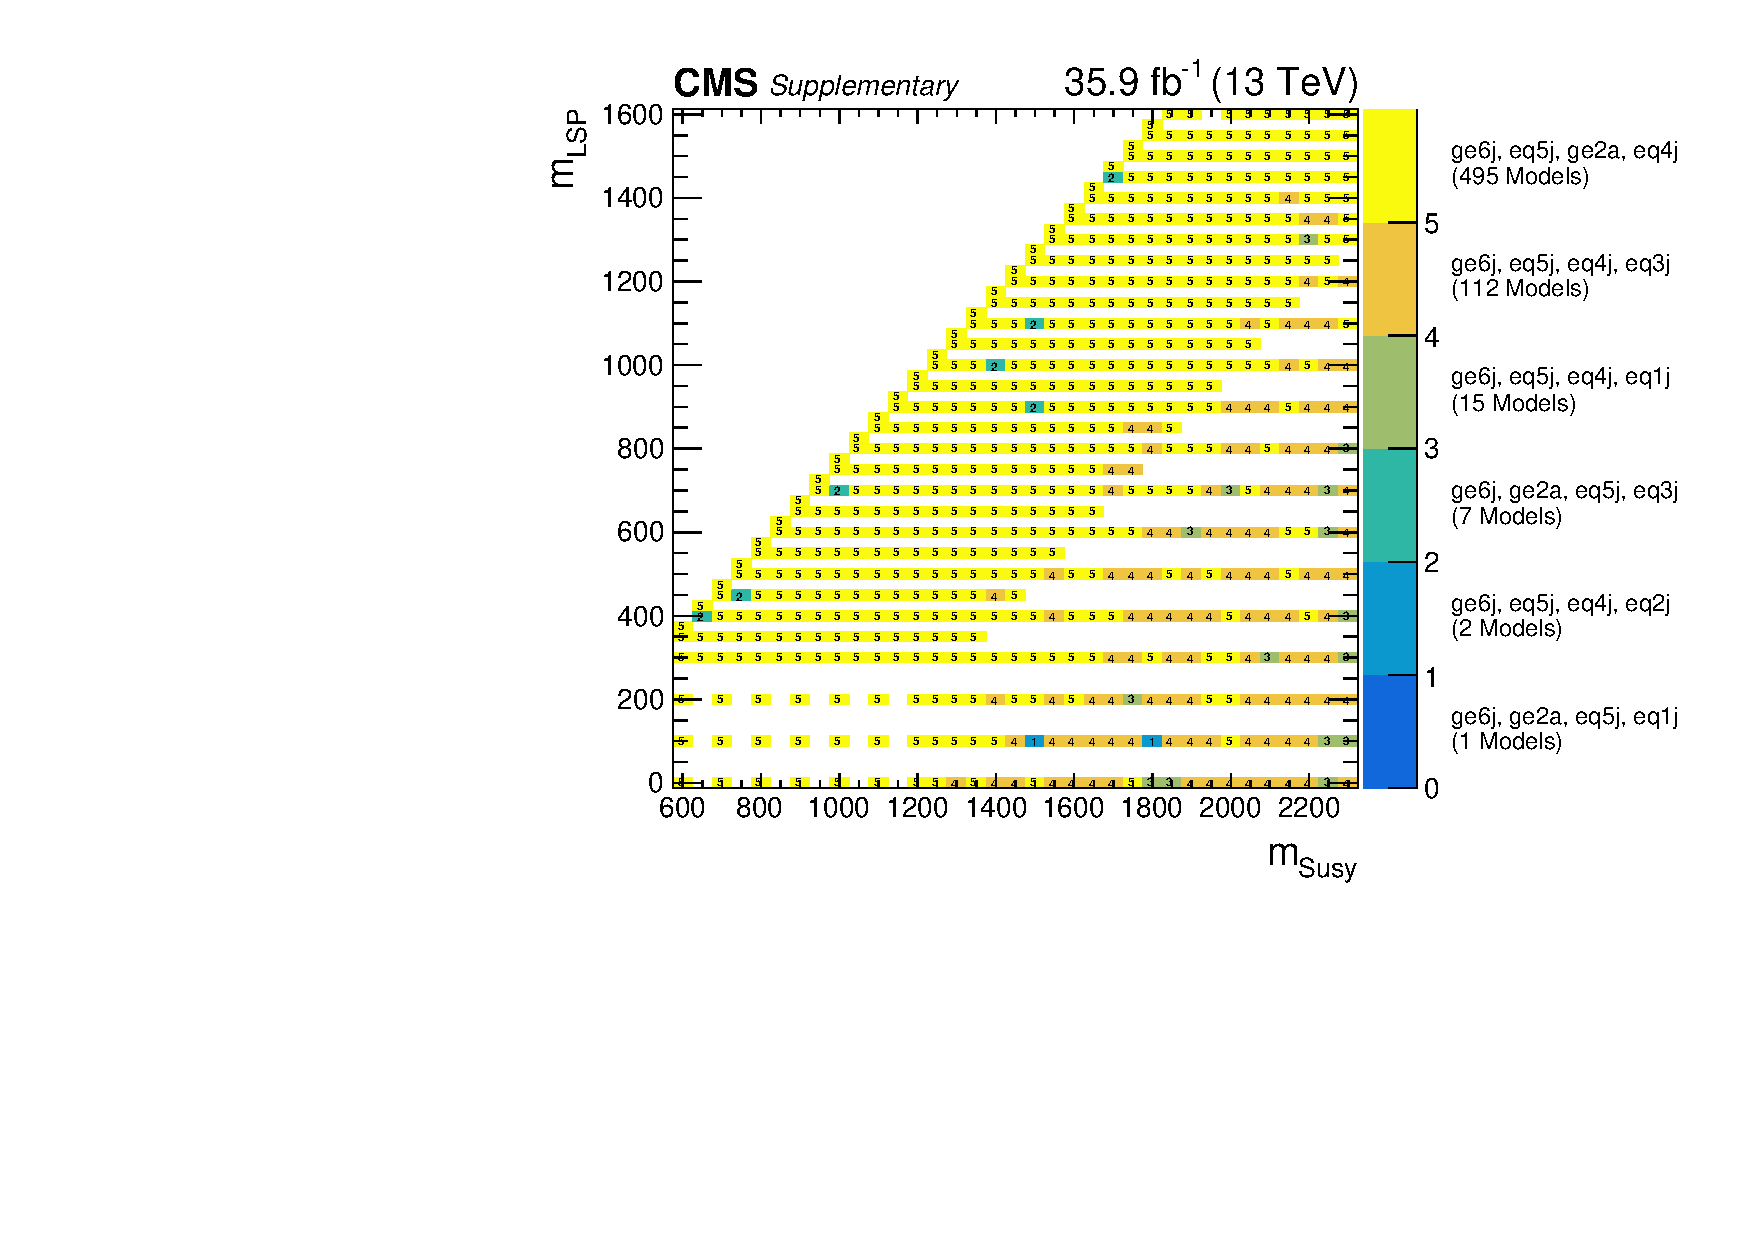
\includegraphics[width=0.45\textwidth]{figures/susyResults/T1tttt_bitMap}
            \label{fig:T1tttt_bitMap}
        } \\
        %\subfigure[T1tttt: Significance scan]{
        %    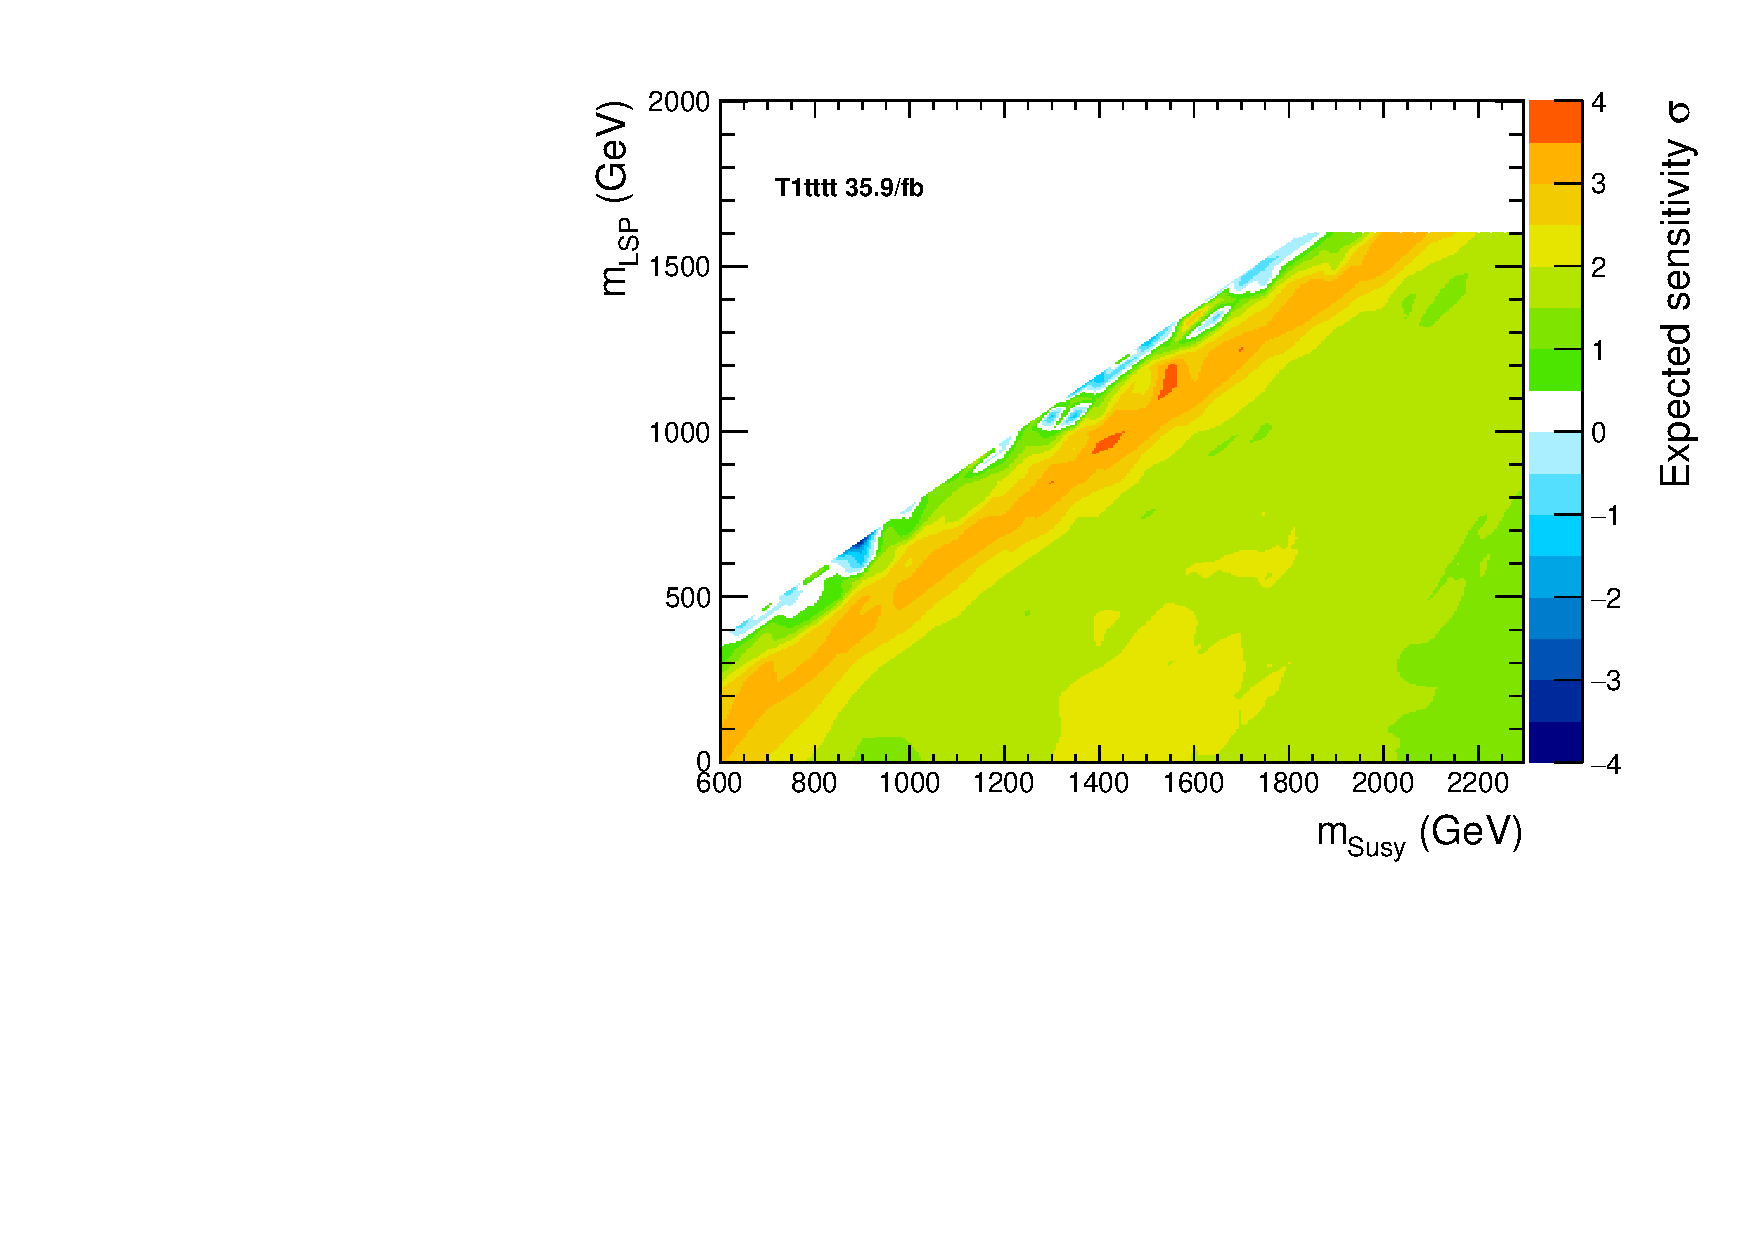
\includegraphics[width=0.45\linewidth]{figures/susyResults/T1tttt_signif}
        %    \label{fig:T1tttt_signif}
        %} ~~
        \caption{Top: the 95\% C.L. observed upper limit on the cross section
            (histogram), with the expected (solid black line) observed
            (solid red line) exclusion contours. Left: signal acceptance
            including all jet categories. Right: graph showing the four
            most sensitive jet categories for each mass point. Bottom:
            local observed significance scan.
        }
        \label{fig:T1tttt}
    \end{center}
\end{figure}

\newpage
\begin{figure}[h!]
    \begin{center}
        \subfigure[T2qq: Upper limit on the cross section in the mass plane]{
            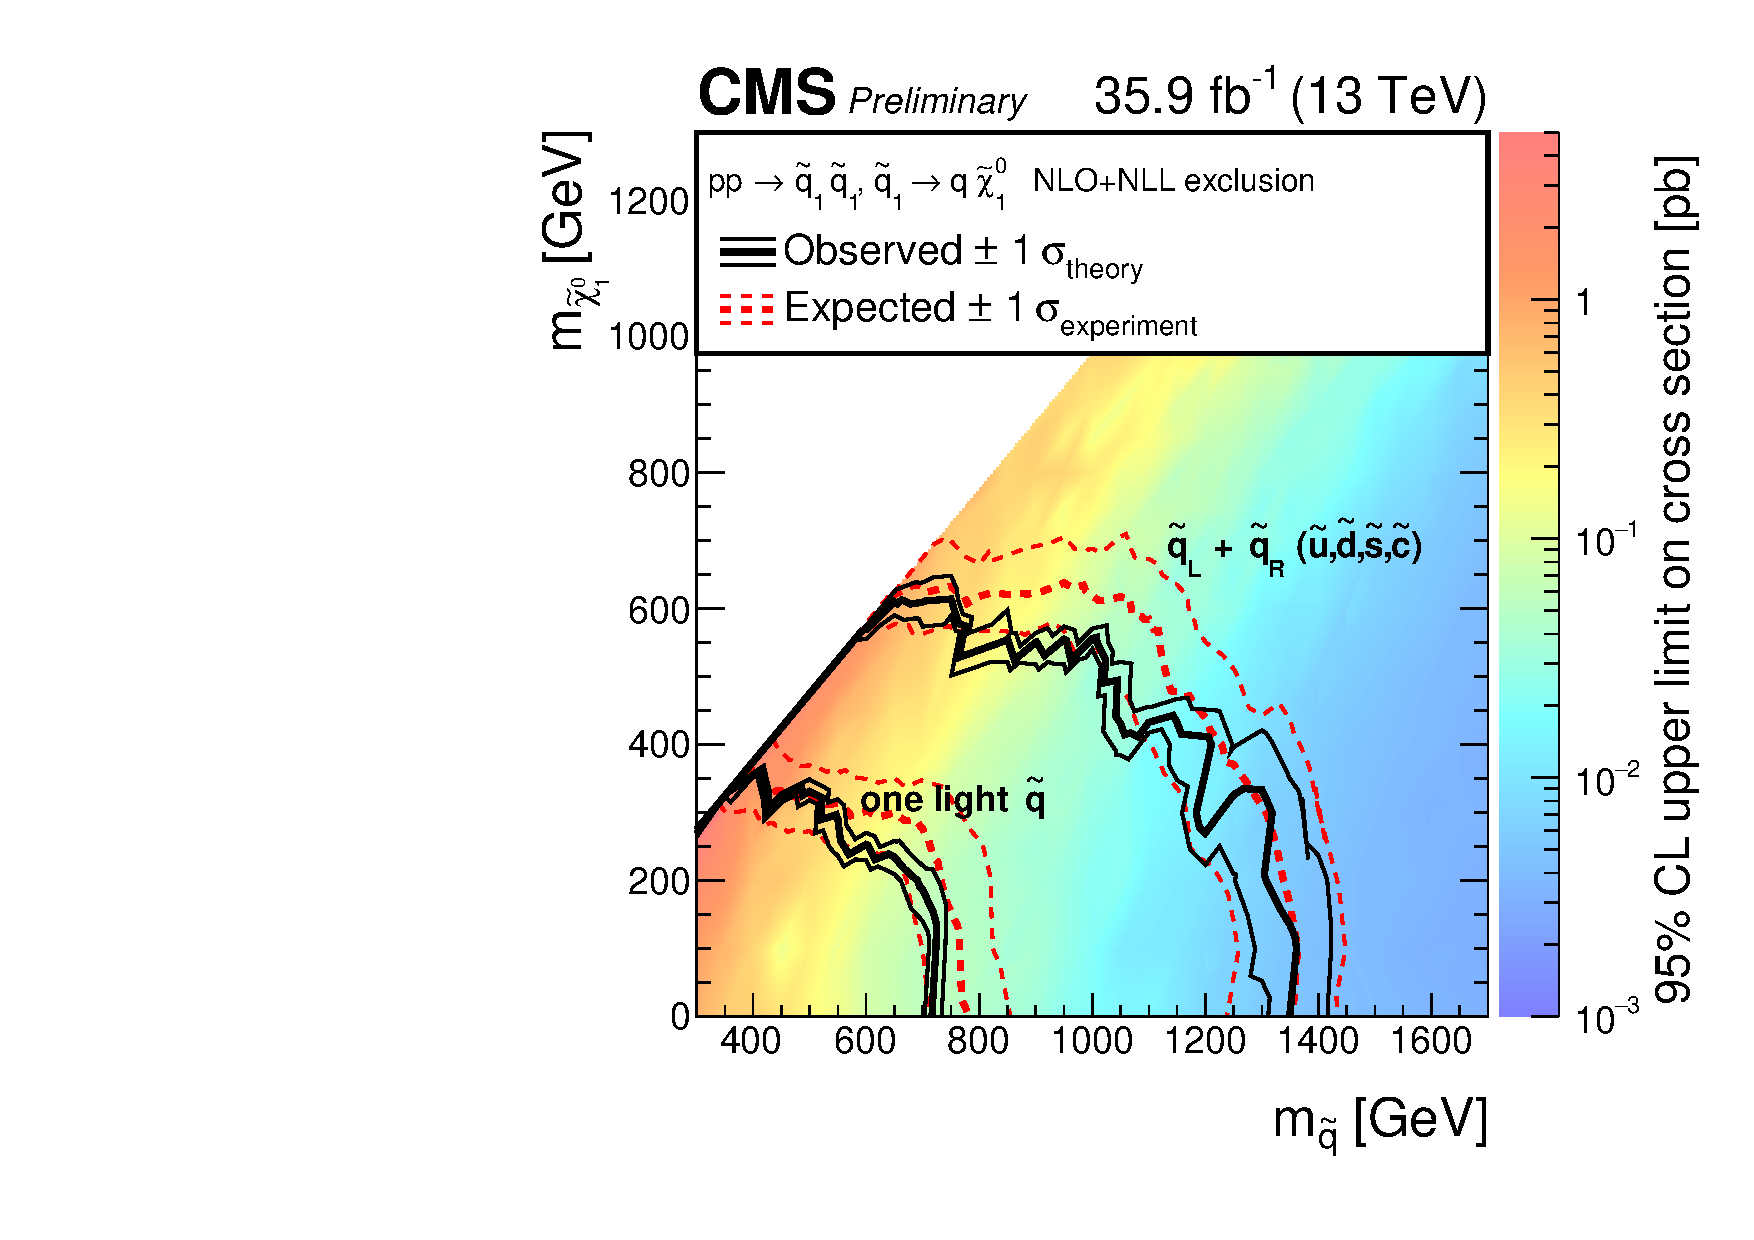
\includegraphics[width=0.6\textwidth]{figures/susyResults/T2qqXSEC}
            \label{fig:T2qq_excl}
        } \\
        \subfigure[T2qq: $\epsilon_{sig}$]{
            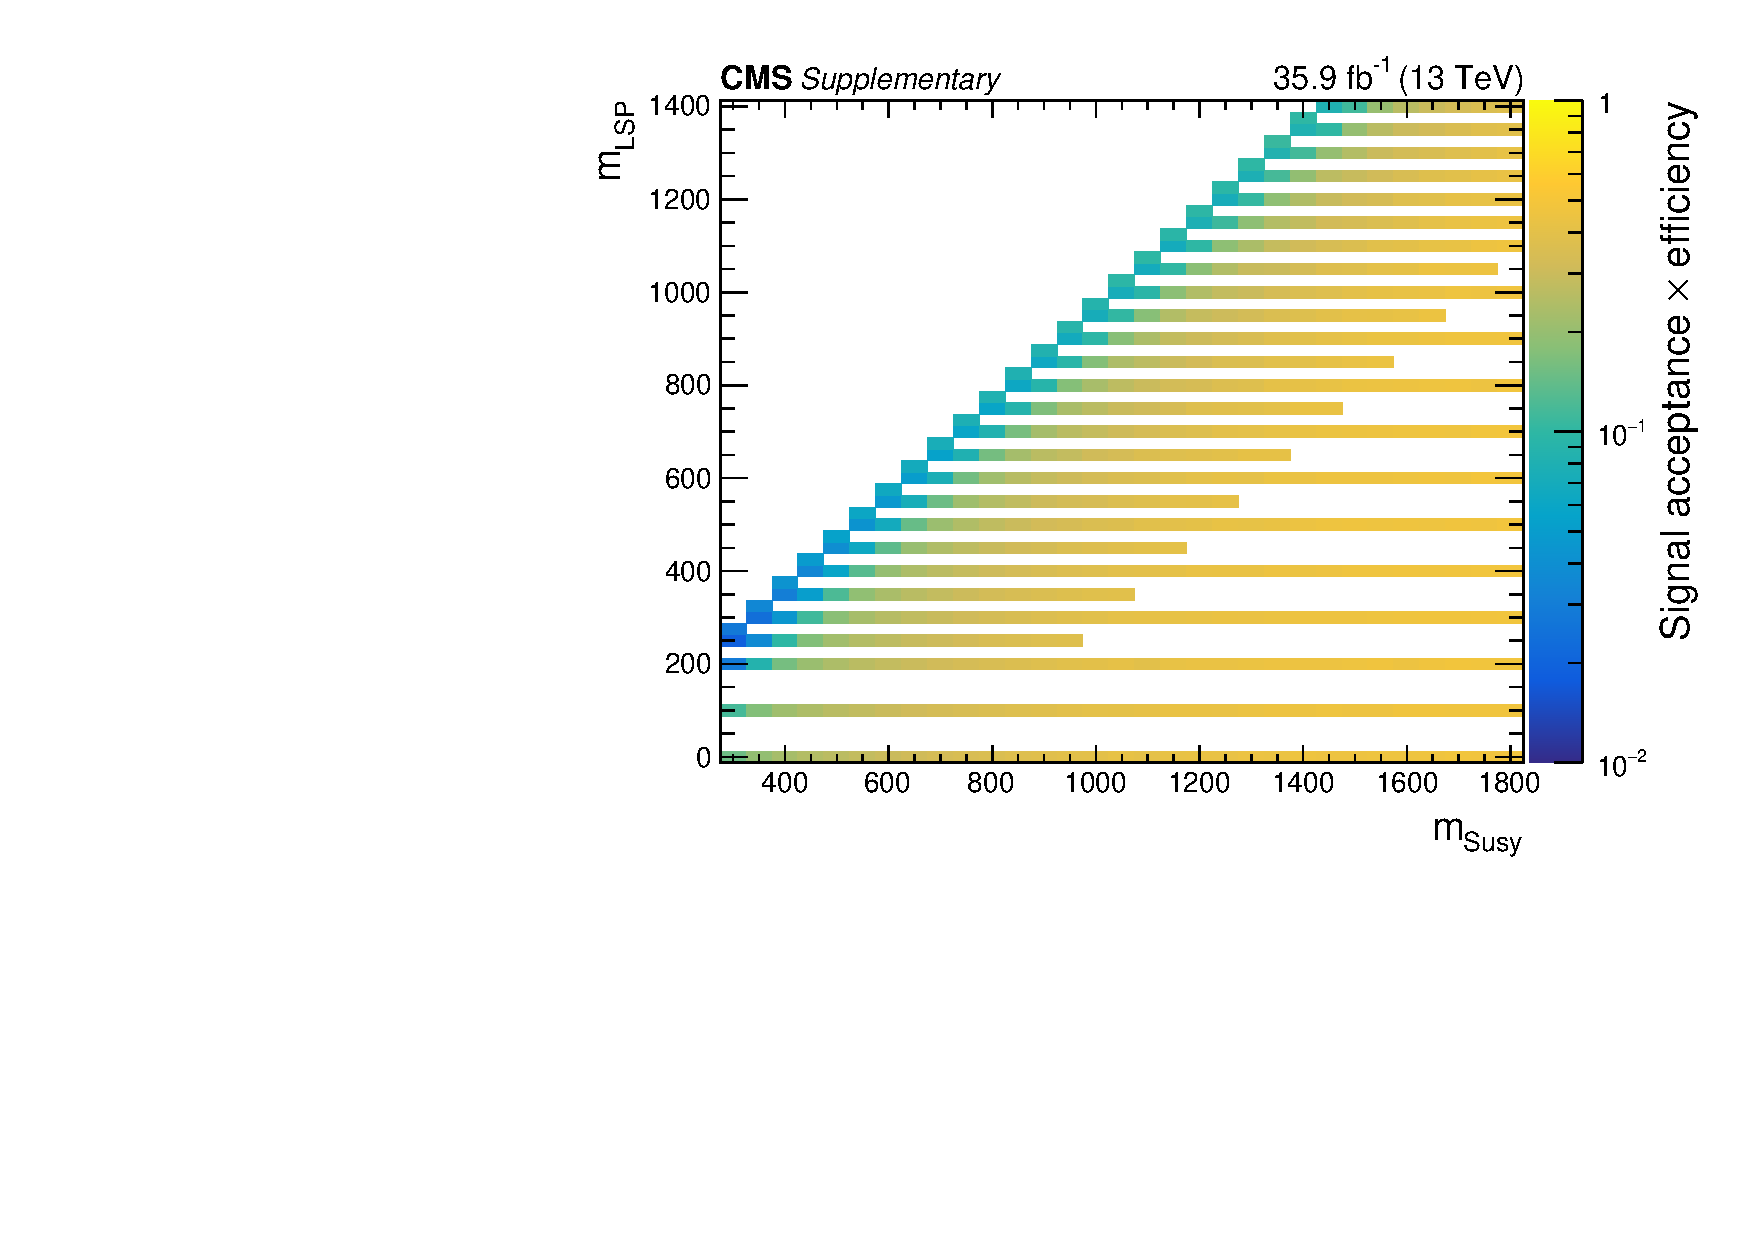
\includegraphics[width=0.45\textwidth]{figures/susyResults/T2qq_effs}
            \label{fig:T2qq_eff}
        } ~~
        \subfigure[T2qq: Most sensitive categories]{
            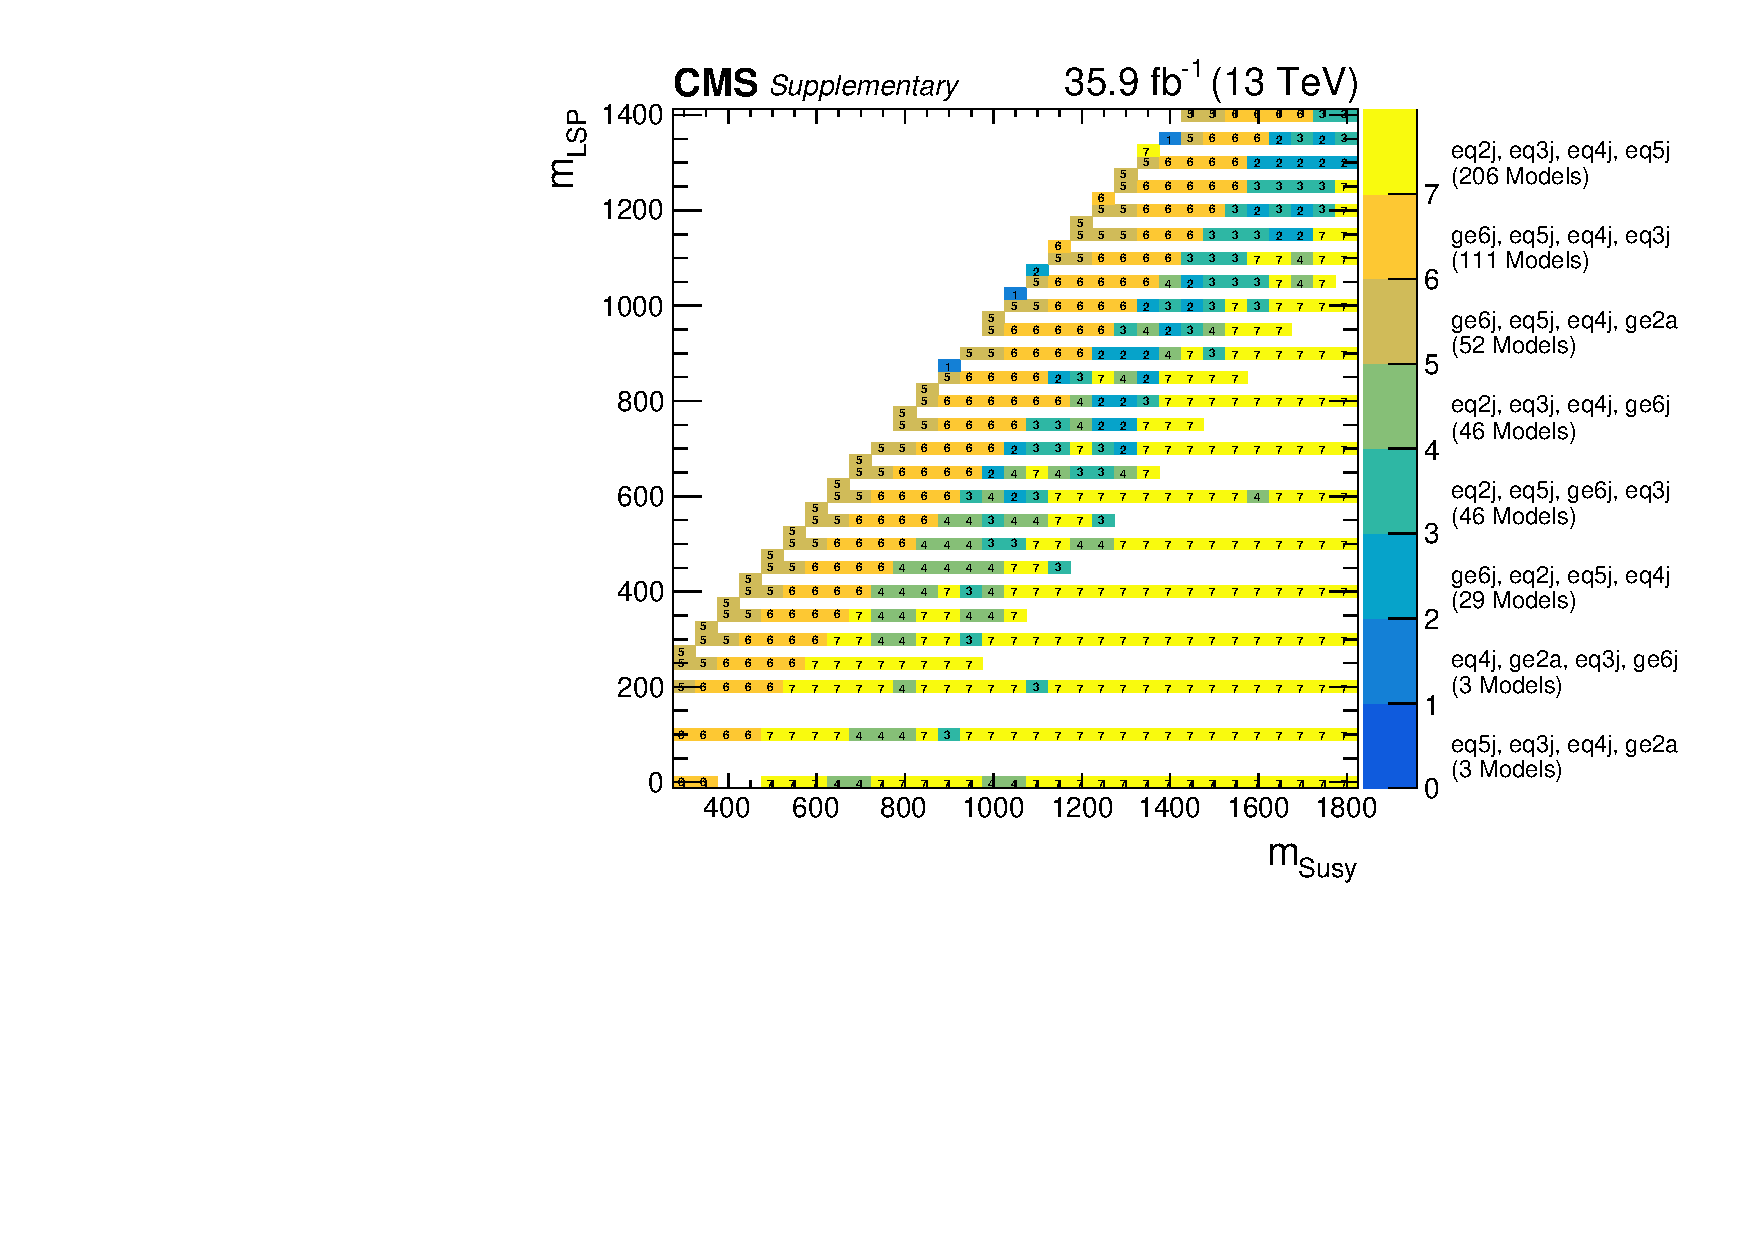
\includegraphics[width=0.45\textwidth]{figures/susyResults/T2qq_bitMap}
            \label{fig:T2qq_bitMap}
        } \\
        \subfigure[T2qq: Significance scan]{
            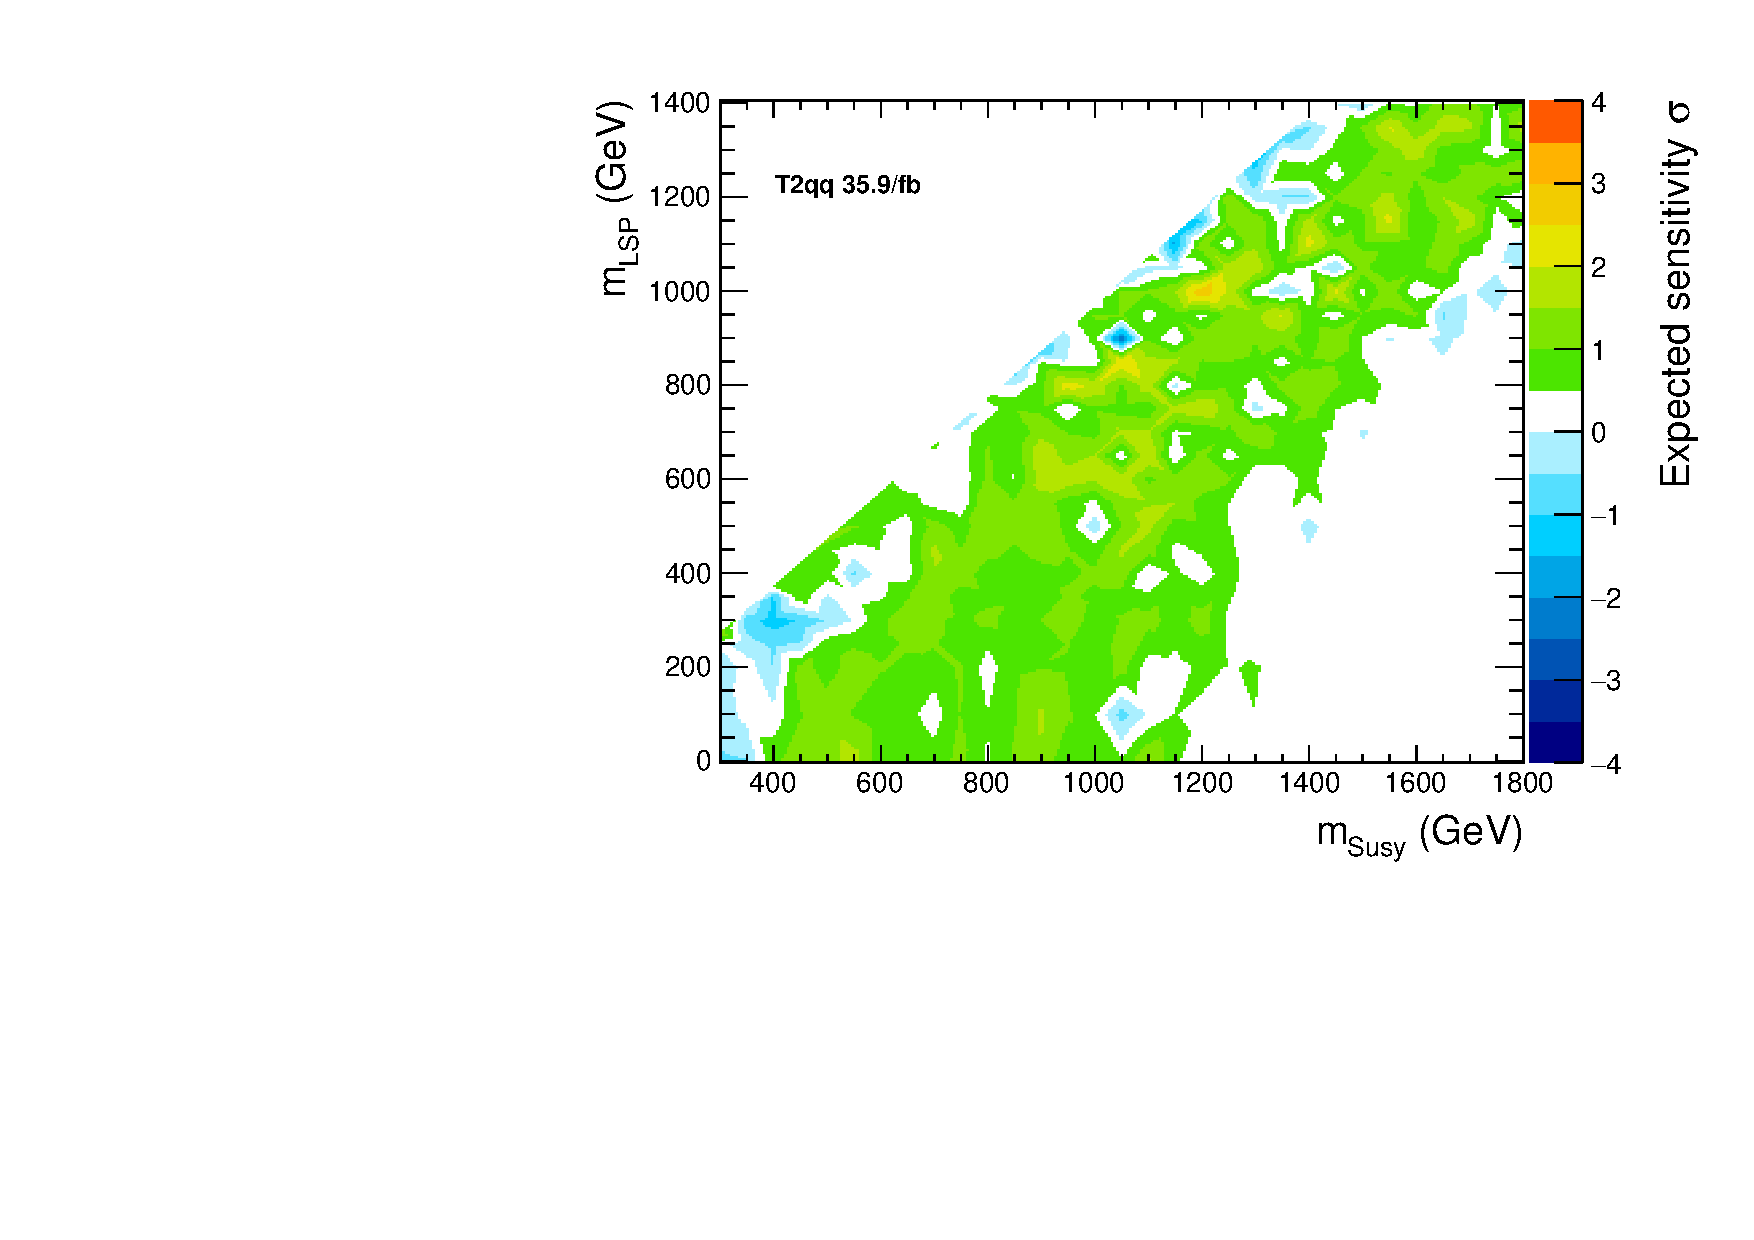
\includegraphics[width=0.45\linewidth]{figures/susyResults/T2qq_signif}
            \label{fig:T2qq_signif}
        } ~~
        \caption{Top: the 95\% C.L. observed upper limit on the cross section
            (histogram), with the expected (solid black line) observed
            (solid red line) exclusion contours. Left: signal acceptance
            including all jet categories. Right: graph showing the four
            most sensitive jet categories for each mass point. Bottom:
            local observed significance scan.
        }
        \label{fig:T2qq}
    \end{center}
\end{figure}

\newpage
\begin{figure}[h!]
    \begin{center}
        \subfigure[T2bb: Upper limit on the cross section in the mass plane]{
            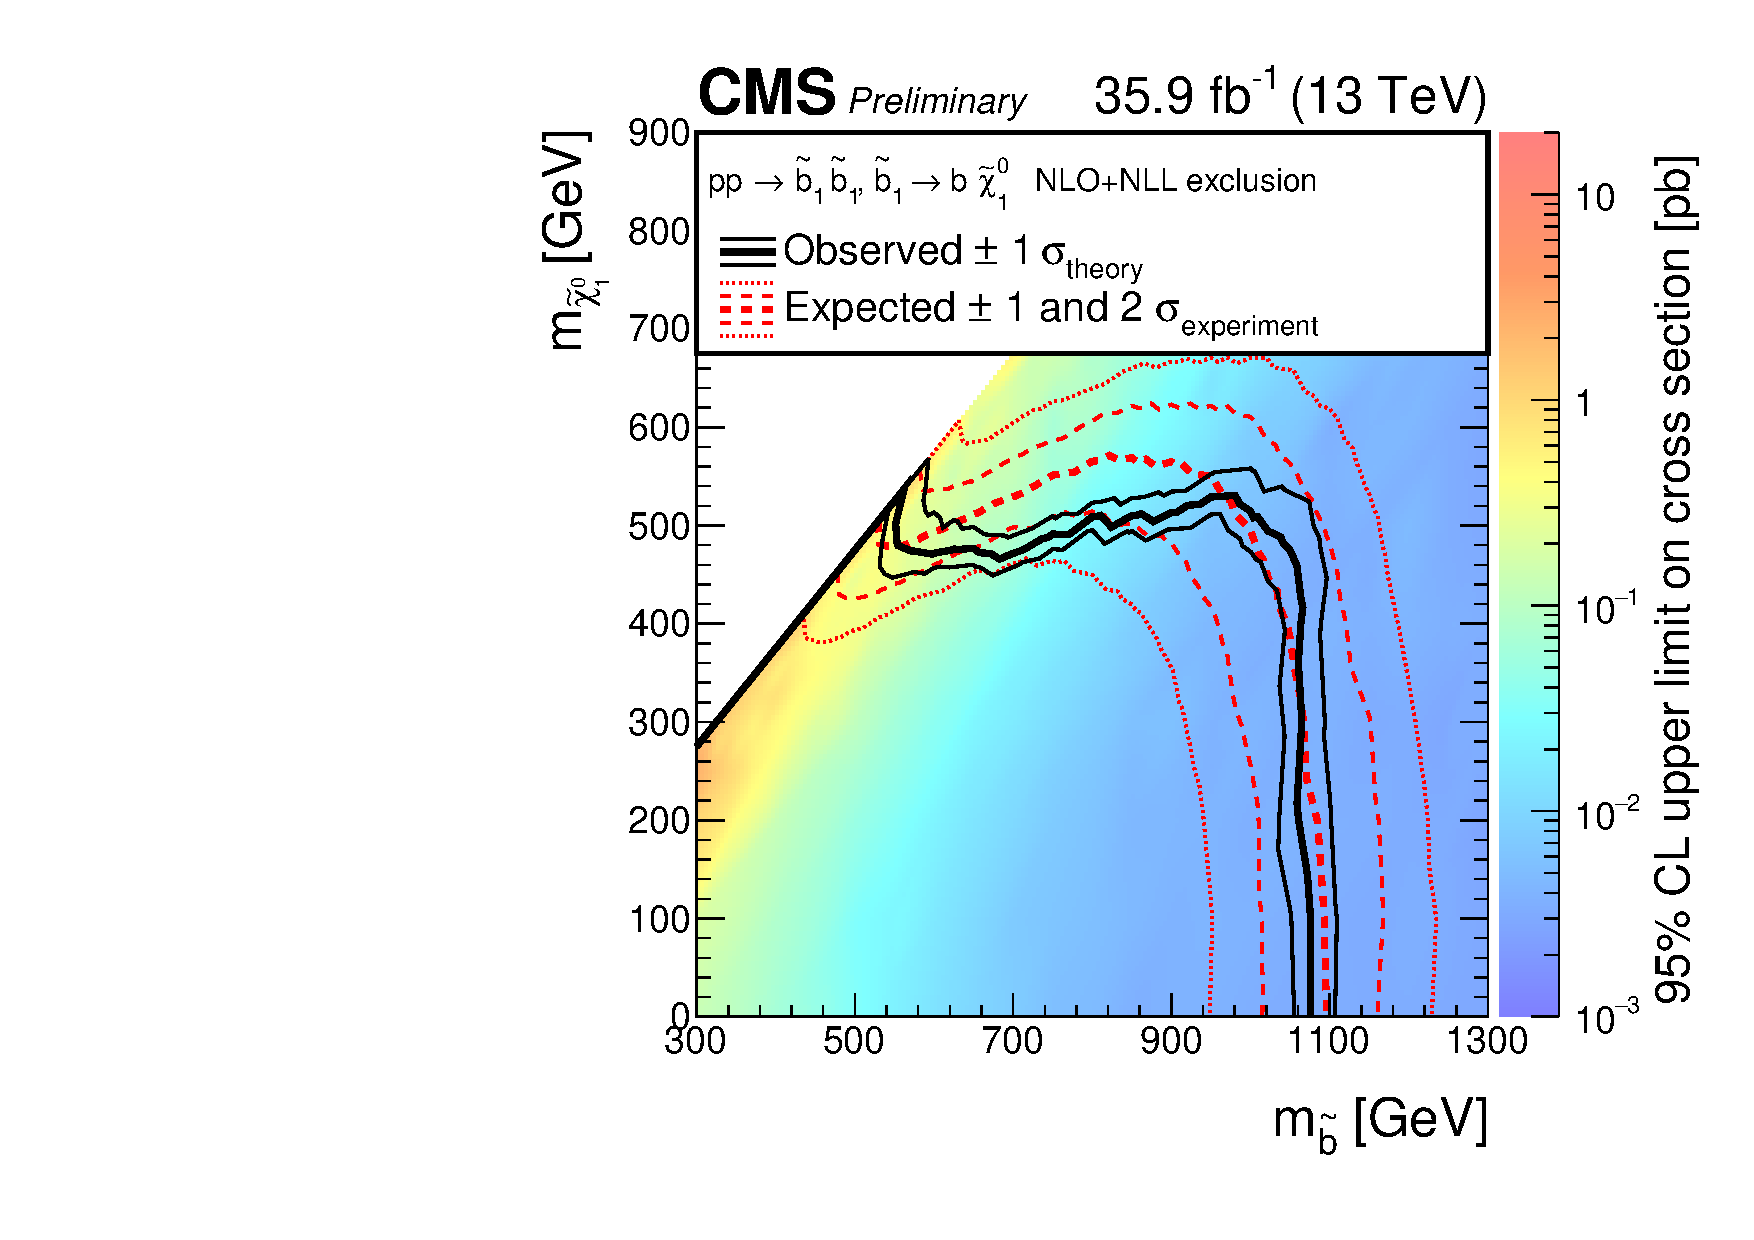
\includegraphics[width=0.6\textwidth]{figures/susyResults/T2bbXSEC}
            \label{fig:T2bb_excl}
        } \\
        \subfigure[T2bb: $\epsilon_{sig}$]{
            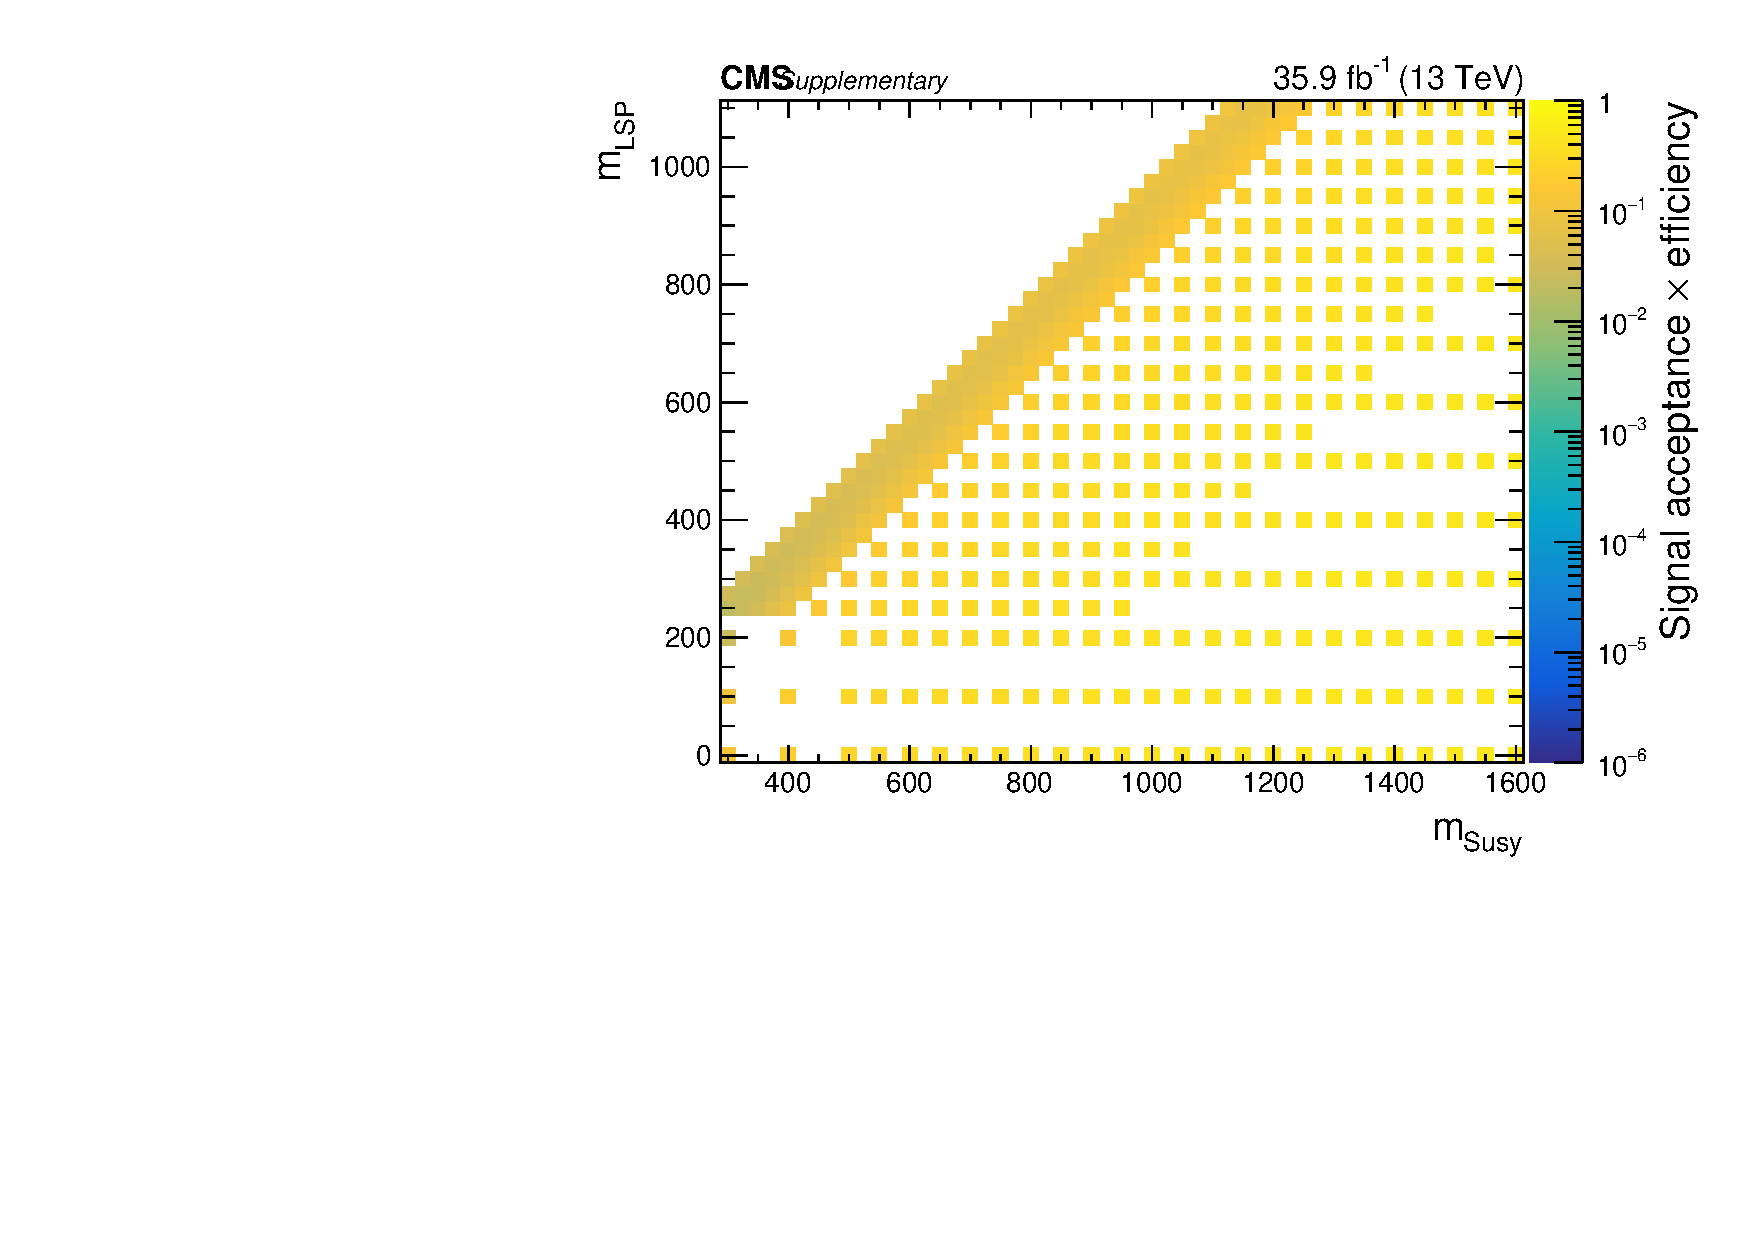
\includegraphics[width=0.45\textwidth]{figures/susyResults/T2bb_effs}
            \label{fig:T2bb_eff}
        } ~~
        \subfigure[T2bb: Most sensitive categories]{
            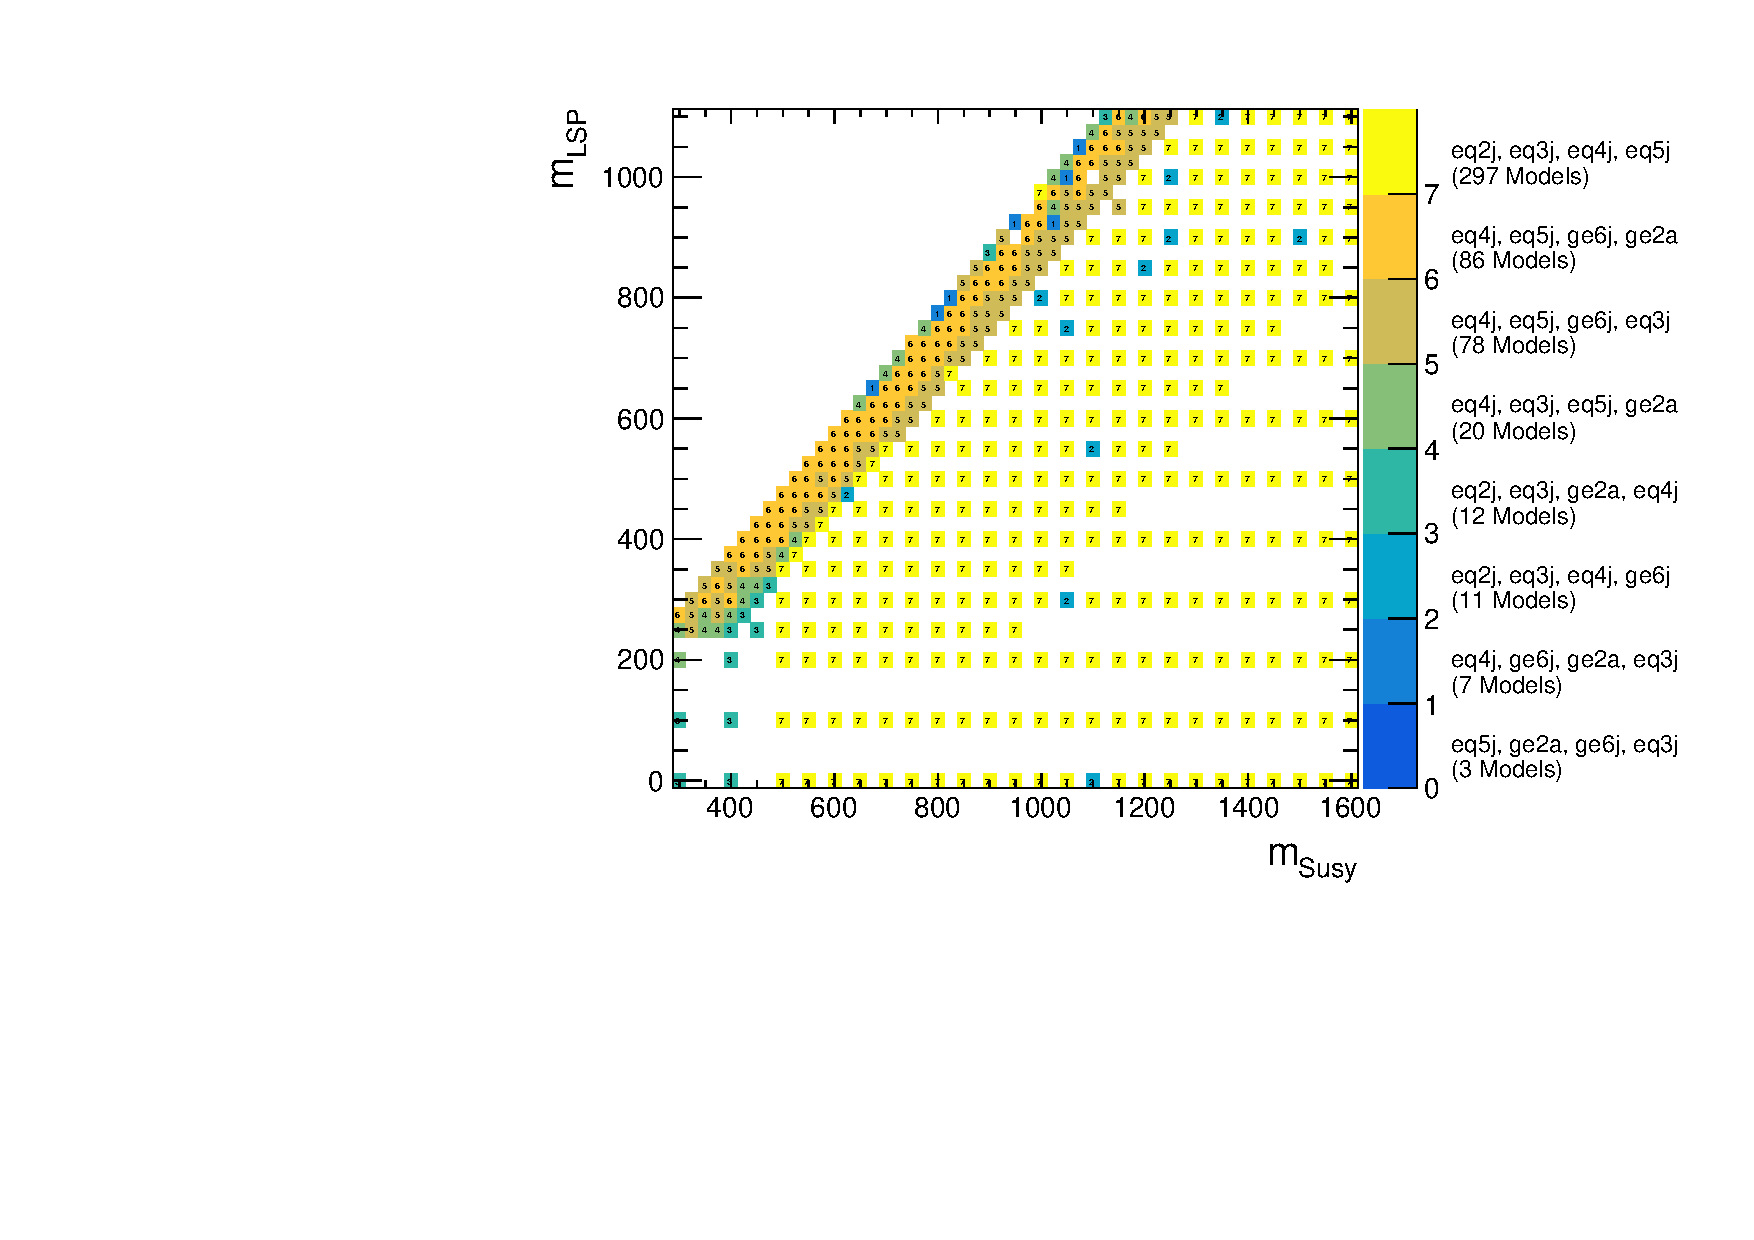
\includegraphics[width=0.45\textwidth]{figures/susyResults/T2bb_bitMap}
            \label{fig:T2bb_bitMap}
        } \\
        \subfigure[T2bb: Significance scan]{
            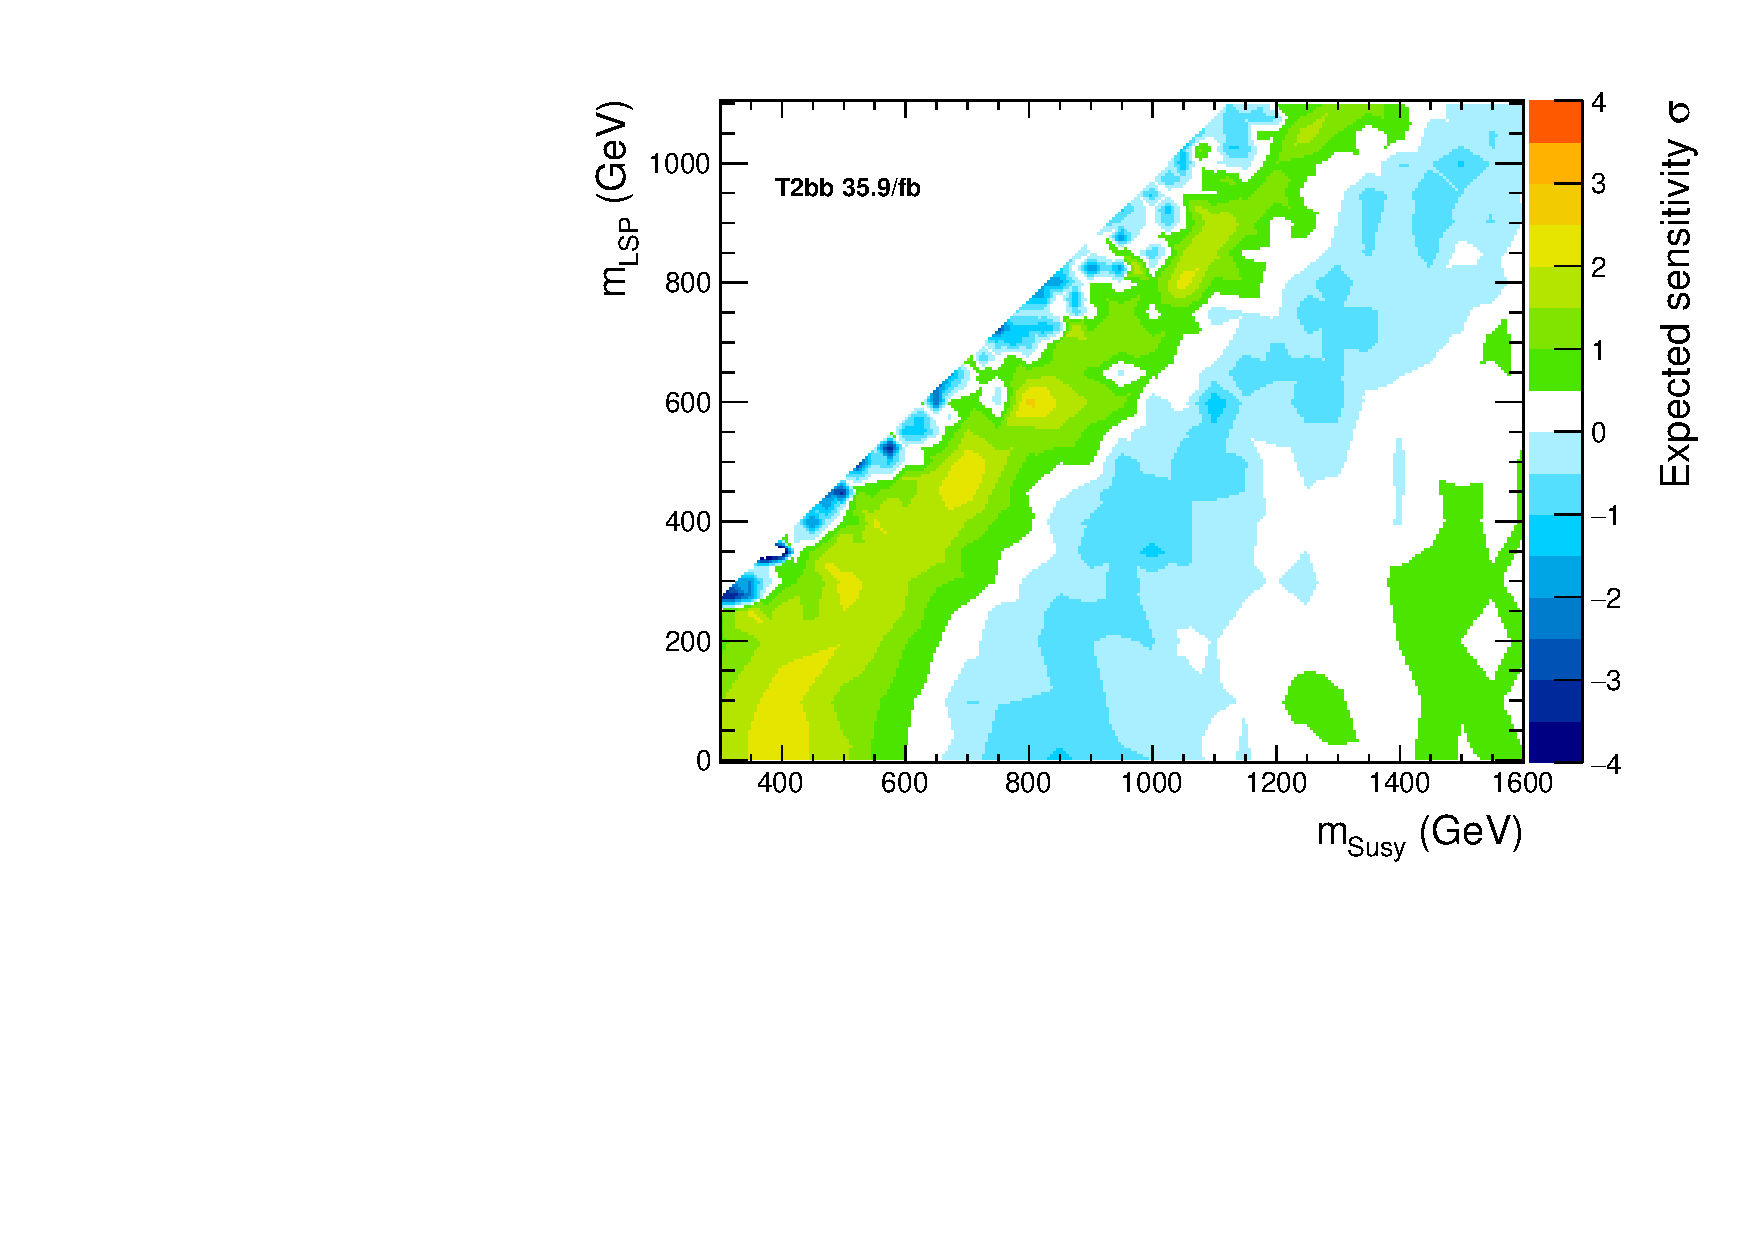
\includegraphics[width=0.45\linewidth]{figures/susyResults/T2bb_signif}
            \label{fig:T2bb_signif}
        } ~~
        \caption{Top: the 95\% C.L. observed upper limit on the cross section
            (histogram), with the expected (solid black line) observed
            (solid red line) exclusion contours. Left: signal acceptance
            including all jet categories. Right: graph showing the four
            most sensitive jet categories for each mass point. Bottom:
            local observed significance scan.
        }
        \label{fig:T2bb}
    \end{center}
\end{figure}

\newpage
\begin{figure}[h!]
    \begin{center}
        \subfigure[T2tt: Upper limit on the cross section in the mass plane]{
            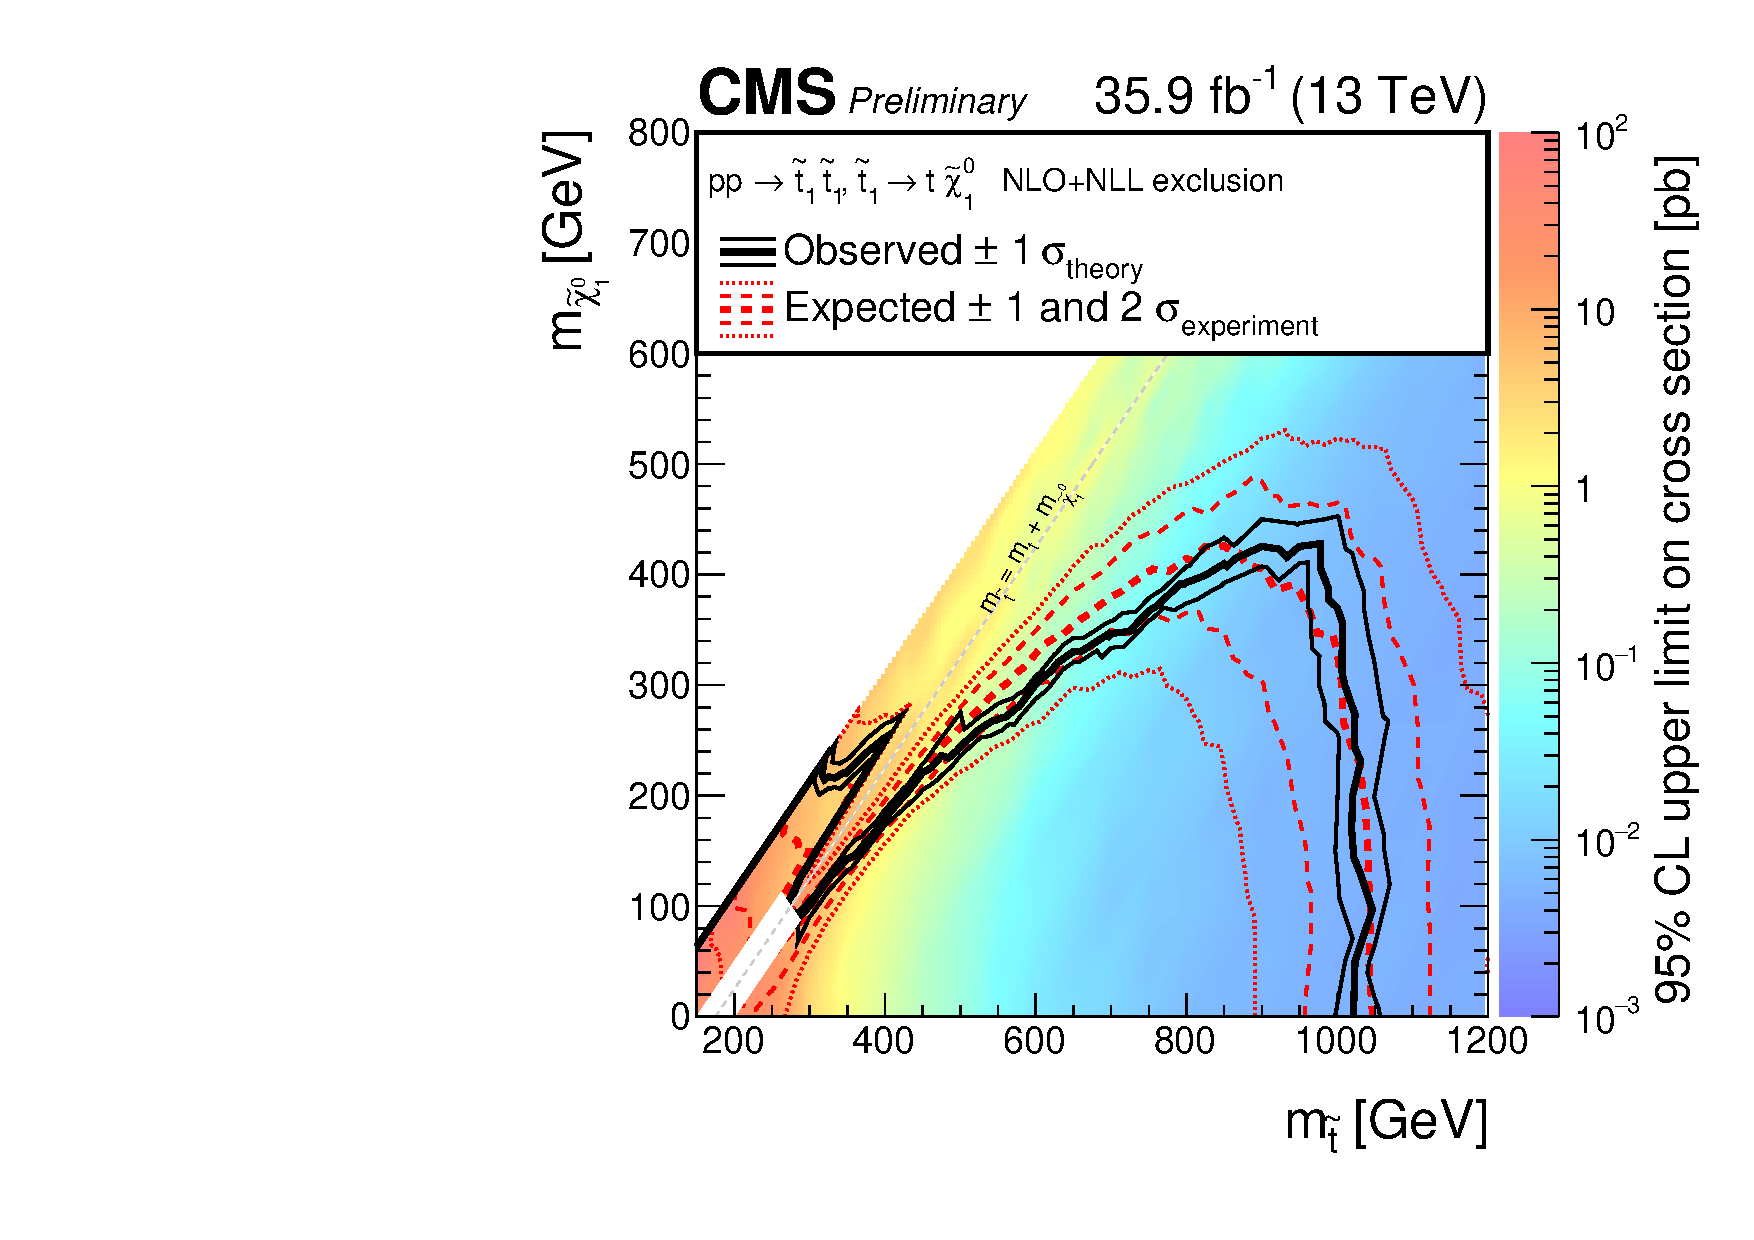
\includegraphics[width=0.6\textwidth]{figures/susyResults/T2ttXSEC}
            \label{fig:T2tt_excl}
        } \\
        \subfigure[T2tt: $\epsilon_{sig}$]{
            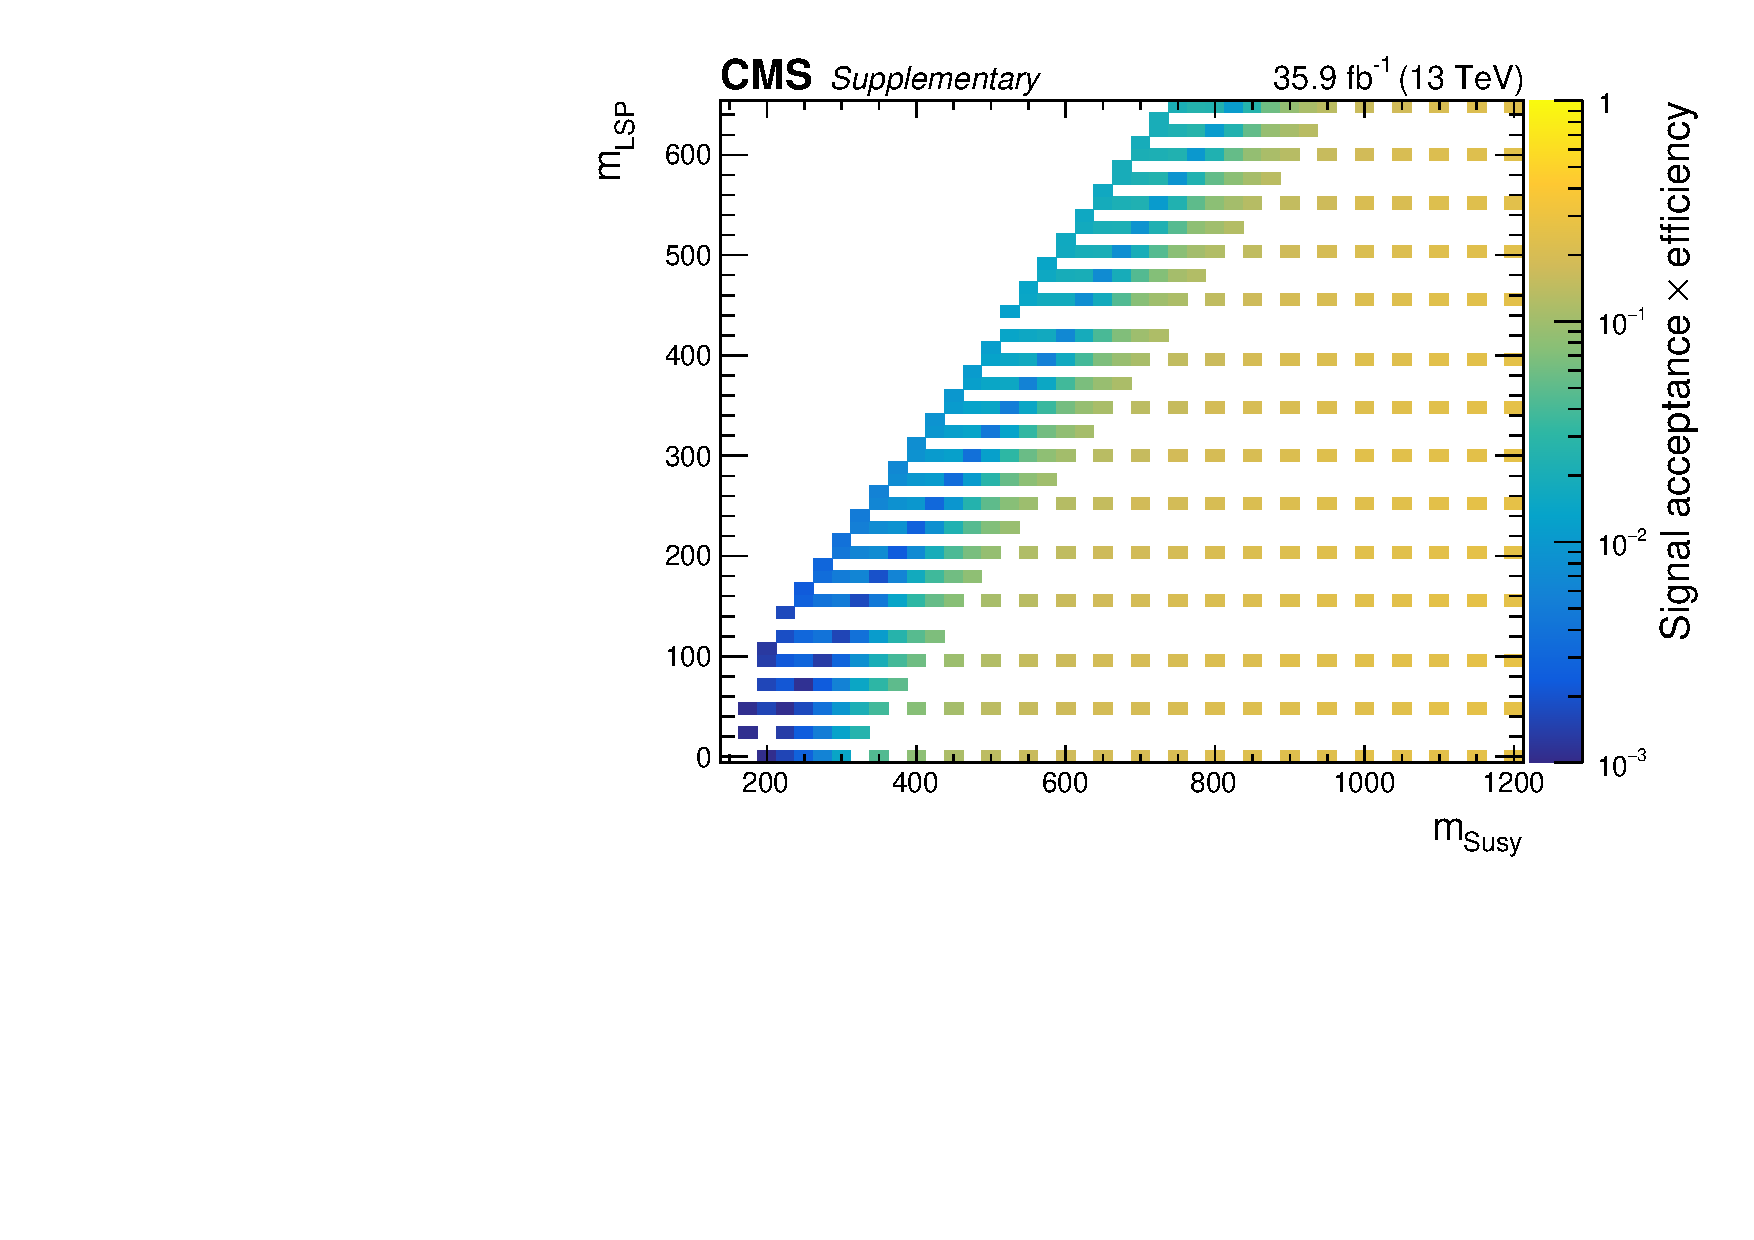
\includegraphics[width=0.45\textwidth]{figures/susyResults/T2tt_effs}
            \label{fig:T2tt_eff}
        } ~~
        \subfigure[T2tt: Most sensitive categories]{
            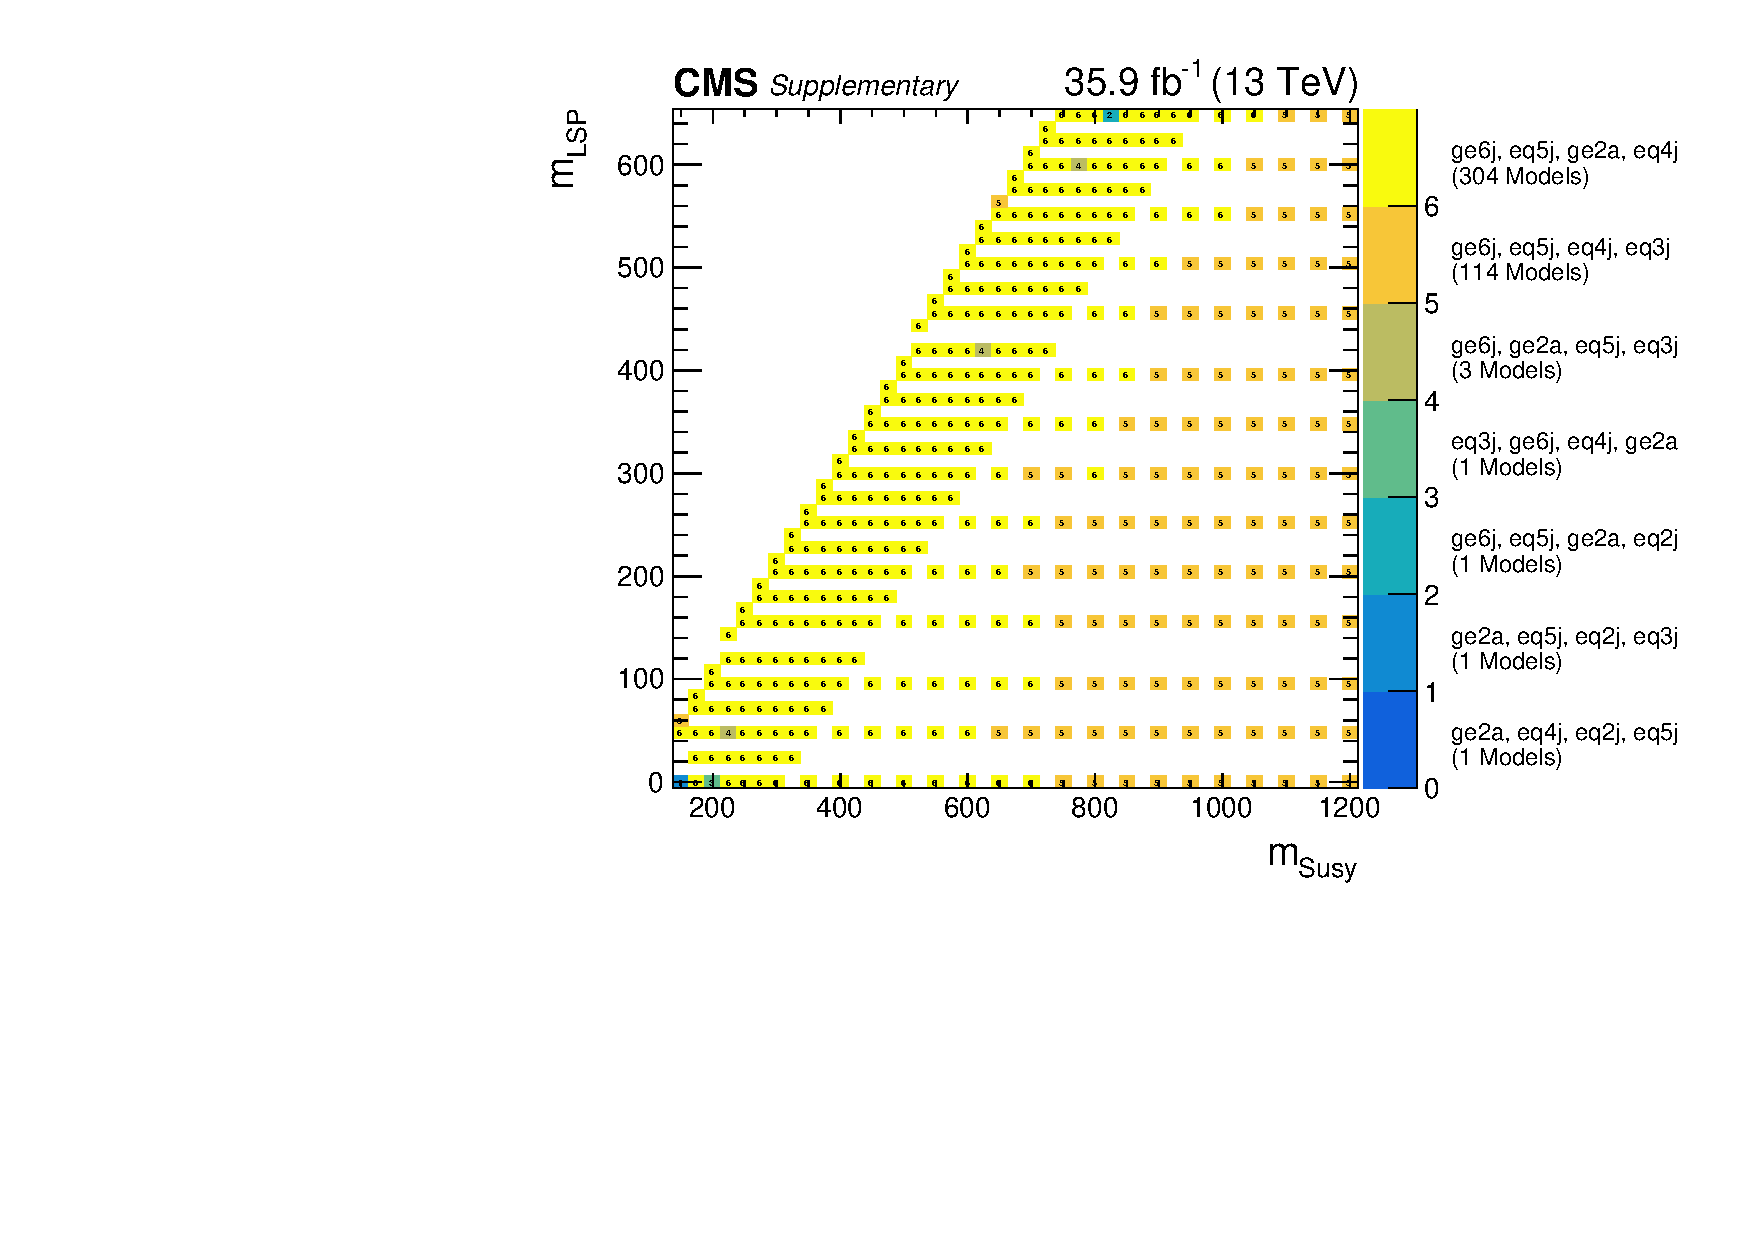
\includegraphics[width=0.45\textwidth]{figures/susyResults/T2tt_bitMap}
            \label{fig:T2tt_bitMap}
        } \\
        \subfigure[T2tt: Significance scan]{
            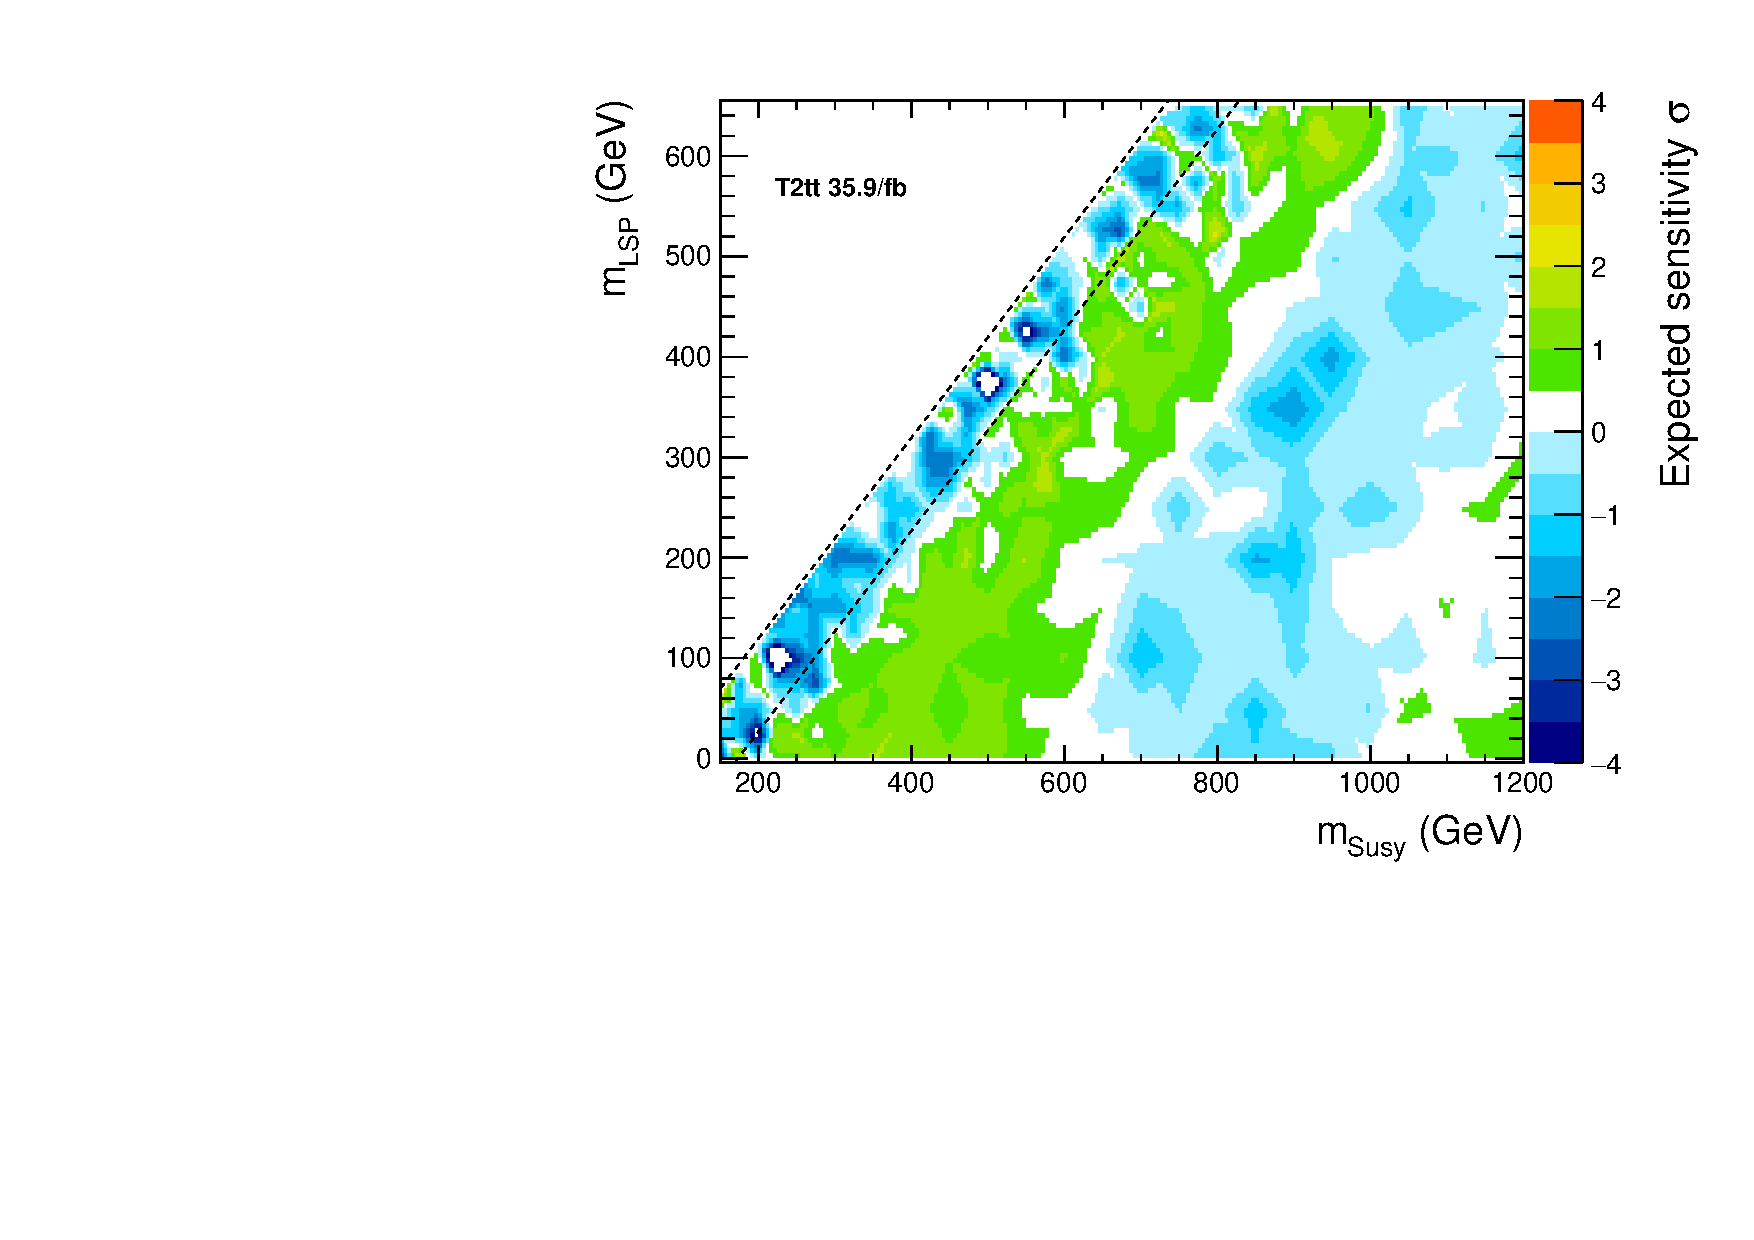
\includegraphics[width=0.45\linewidth]{figures/susyResults/T2tt_signif}
            \label{fig:T2tt_signif}
        } ~~
        \caption{Top: the 95\% C.L. observed upper limit on the cross section
            (histogram), with the expected (solid black line) observed
            (solid red line) exclusion contours. Left: signal acceptance
            including all jet categories. Right: graph showing the four
            most sensitive jet categories for each mass point. Bottom:
            local observed significance scan.
        }
        \label{fig:T2tt}
    \end{center}
\end{figure}

\newpage
\begin{figure}[h!]
    \begin{center}
        \subfigure[T2cc: Upper limit on the cross section in the mass plane]{
            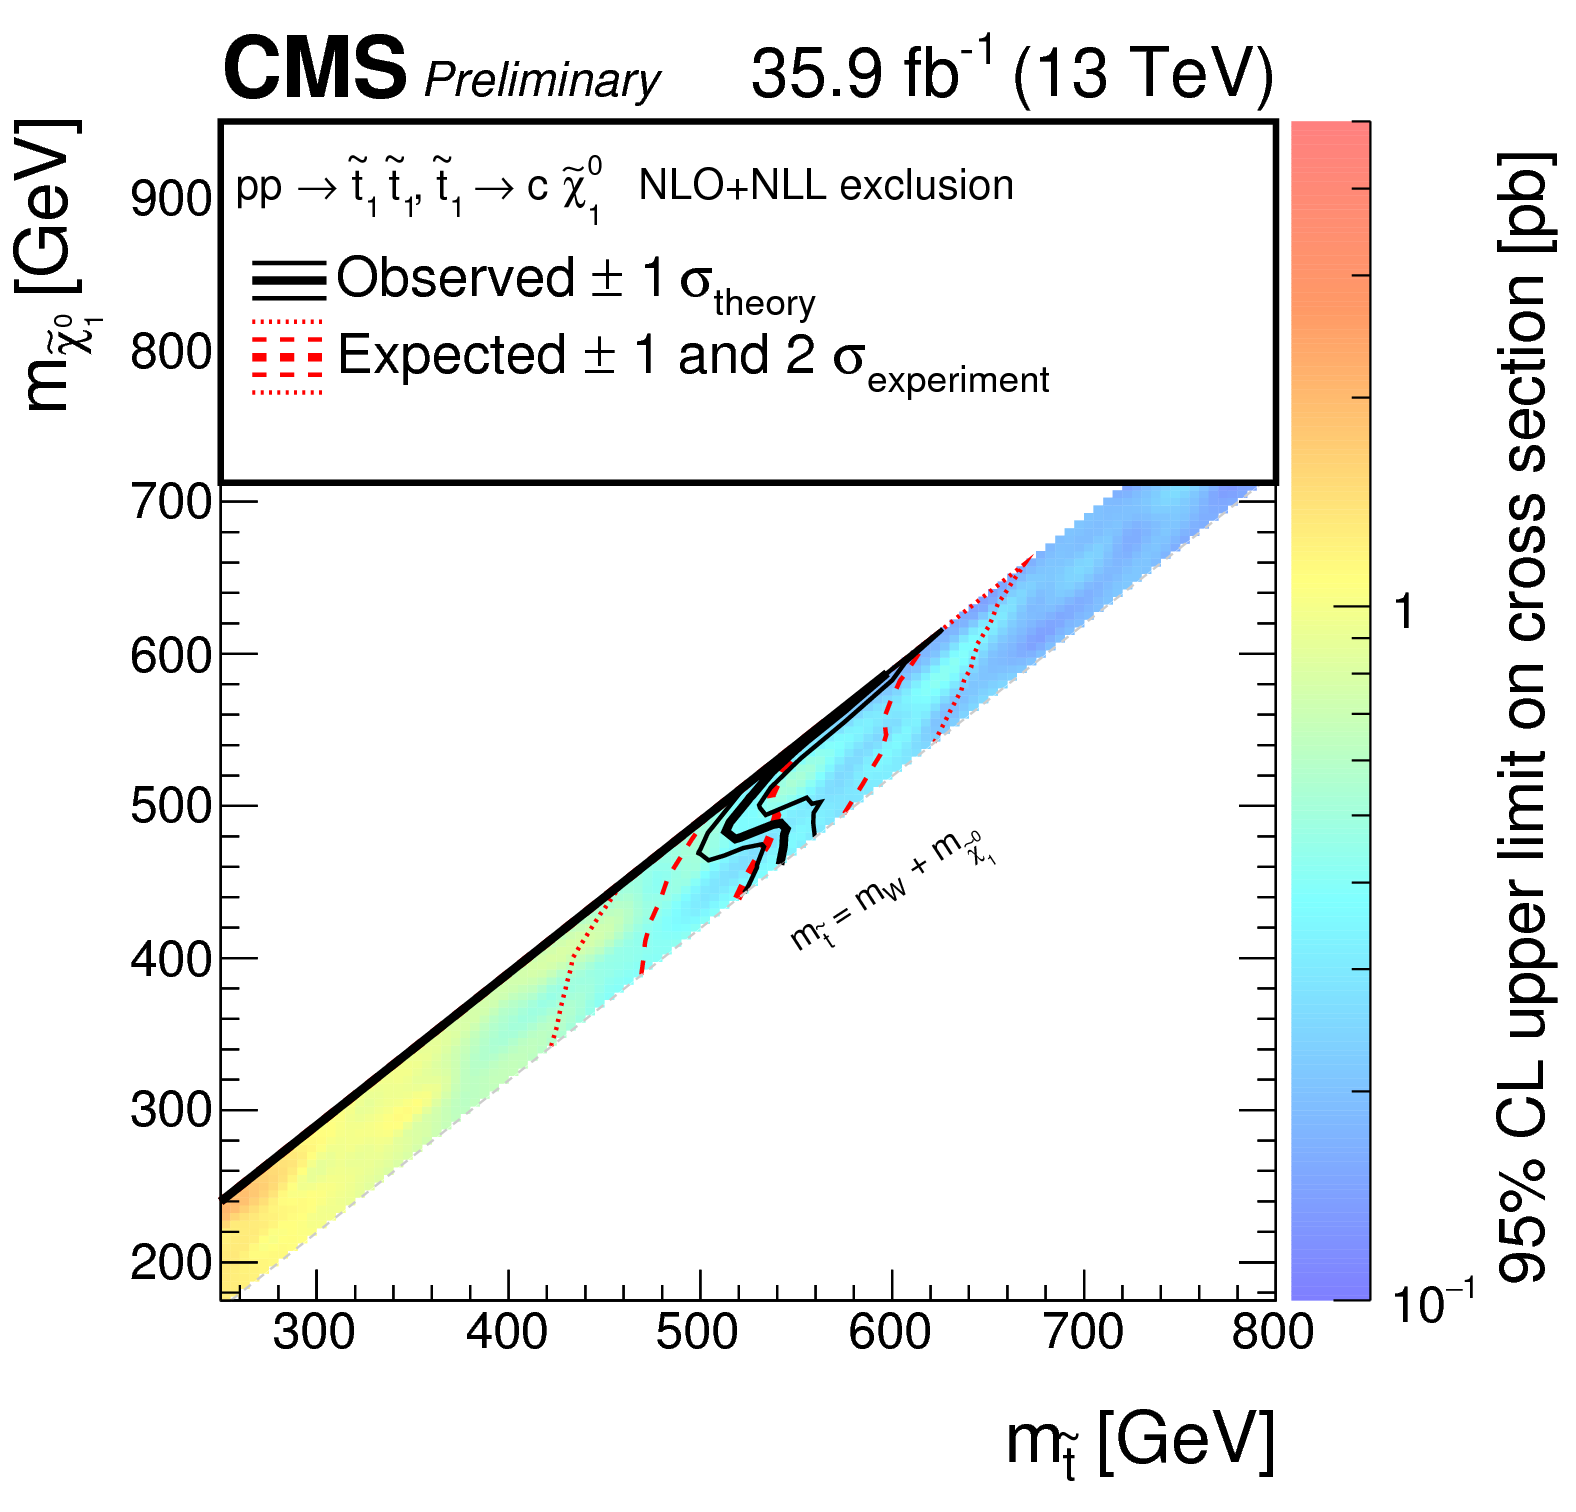
\includegraphics[width=0.6\textwidth]{figures/susyResults/T2ccXSEC}
            \label{fig:T2cc_excl}
        } \\
        \subfigure[T2cc: $\epsilon_{sig}$]{
            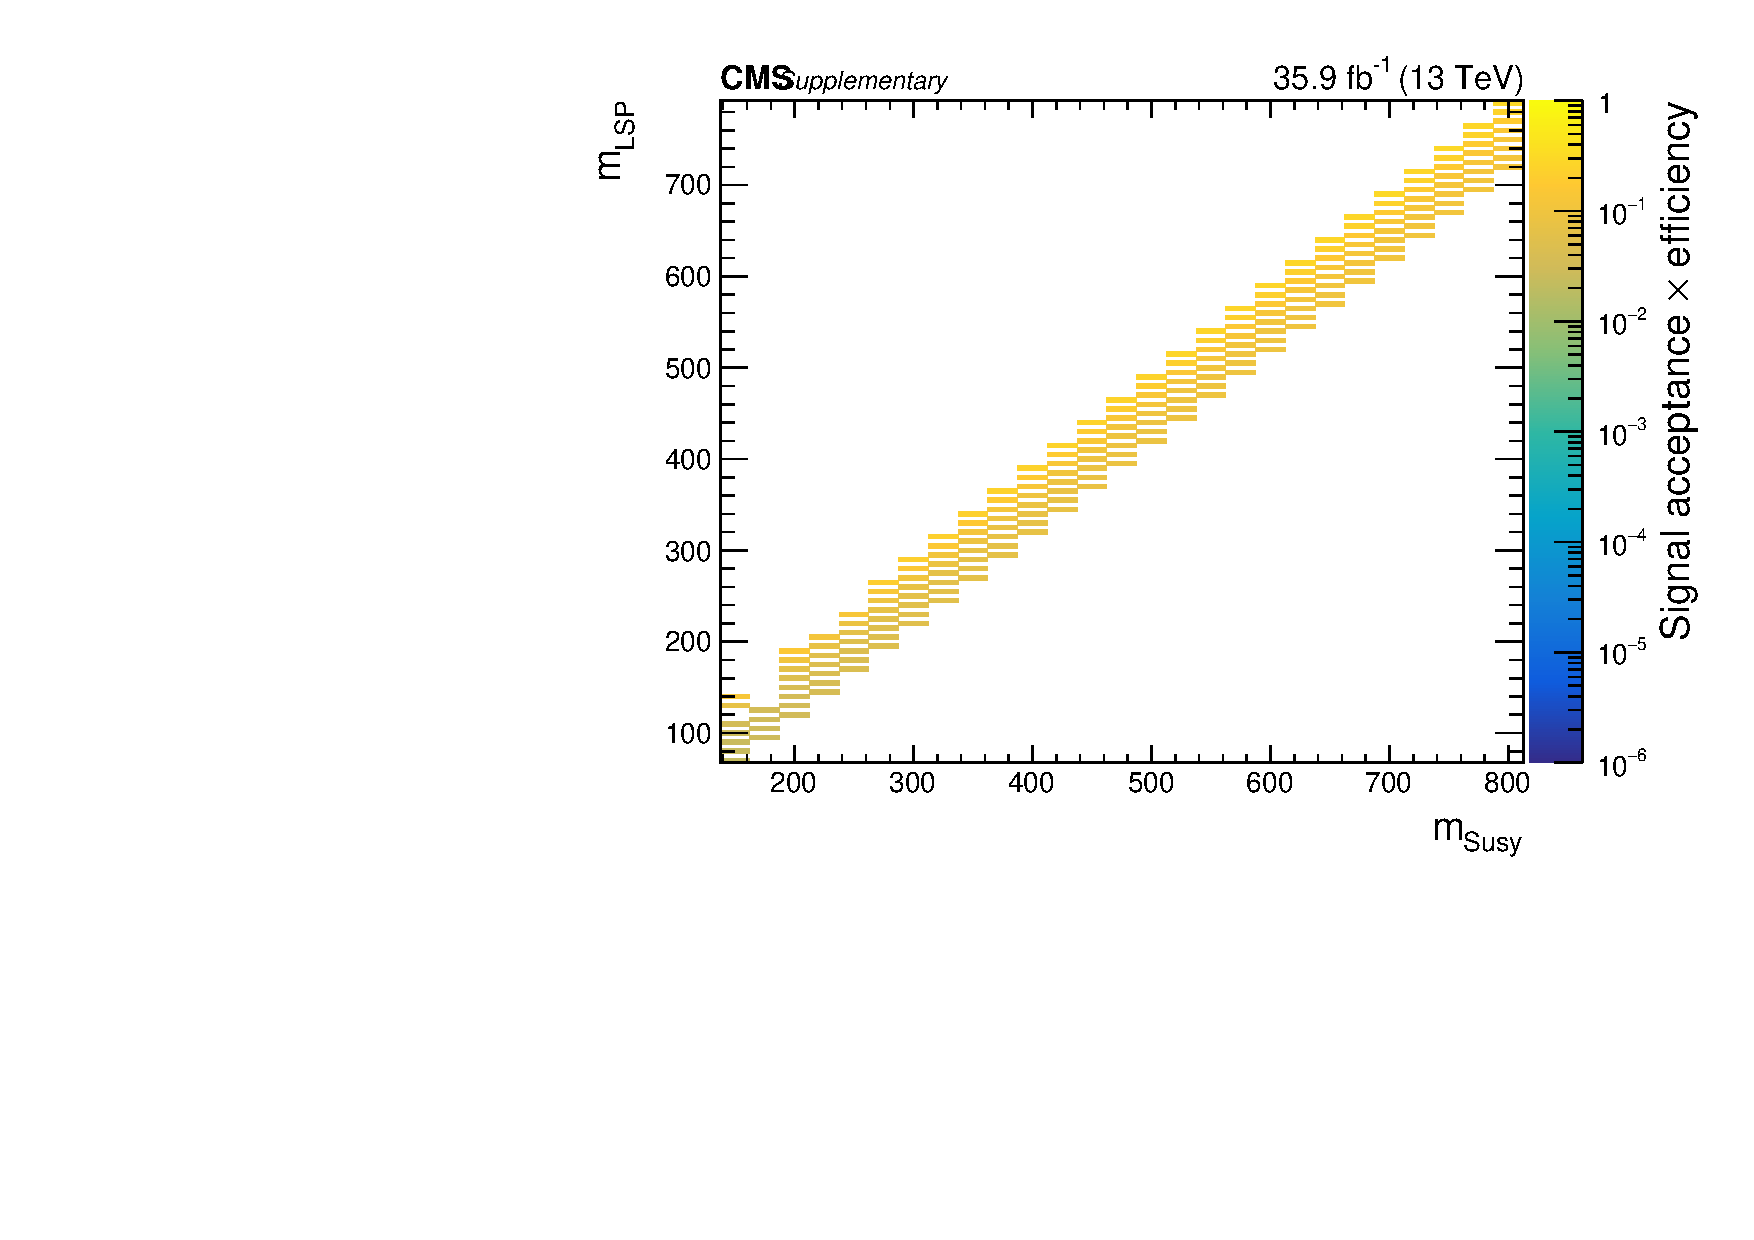
\includegraphics[width=0.45\textwidth]{figures/susyResults/T2cc_effs}
            \label{fig:T2cc_eff}
        } ~~
        \subfigure[T2cc: Most sensitive categories]{
            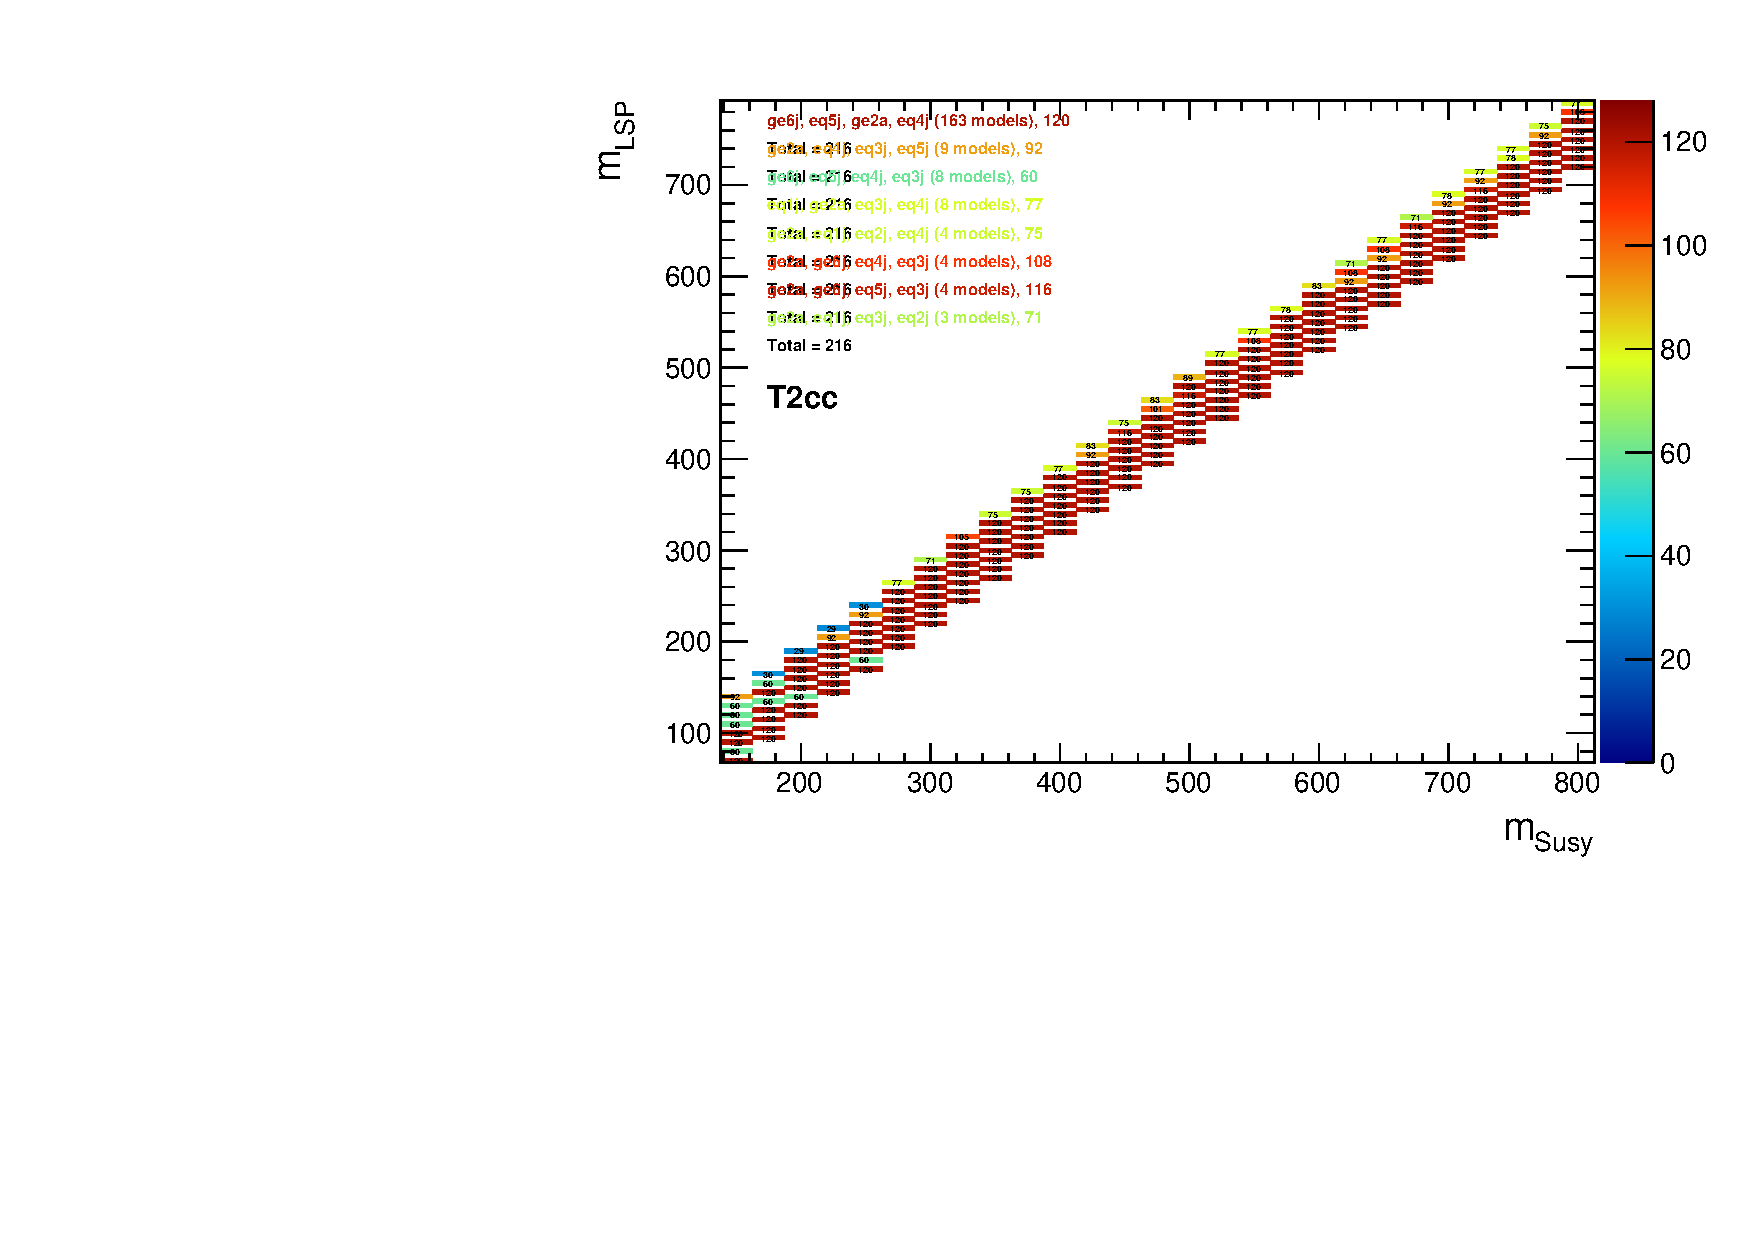
\includegraphics[width=0.45\textwidth]{figures/susyResults/T2cc_bitMap}
            \label{fig:T2cc_bitMap}
        } \\
        \subfigure[T2cc: Significance scan]{
            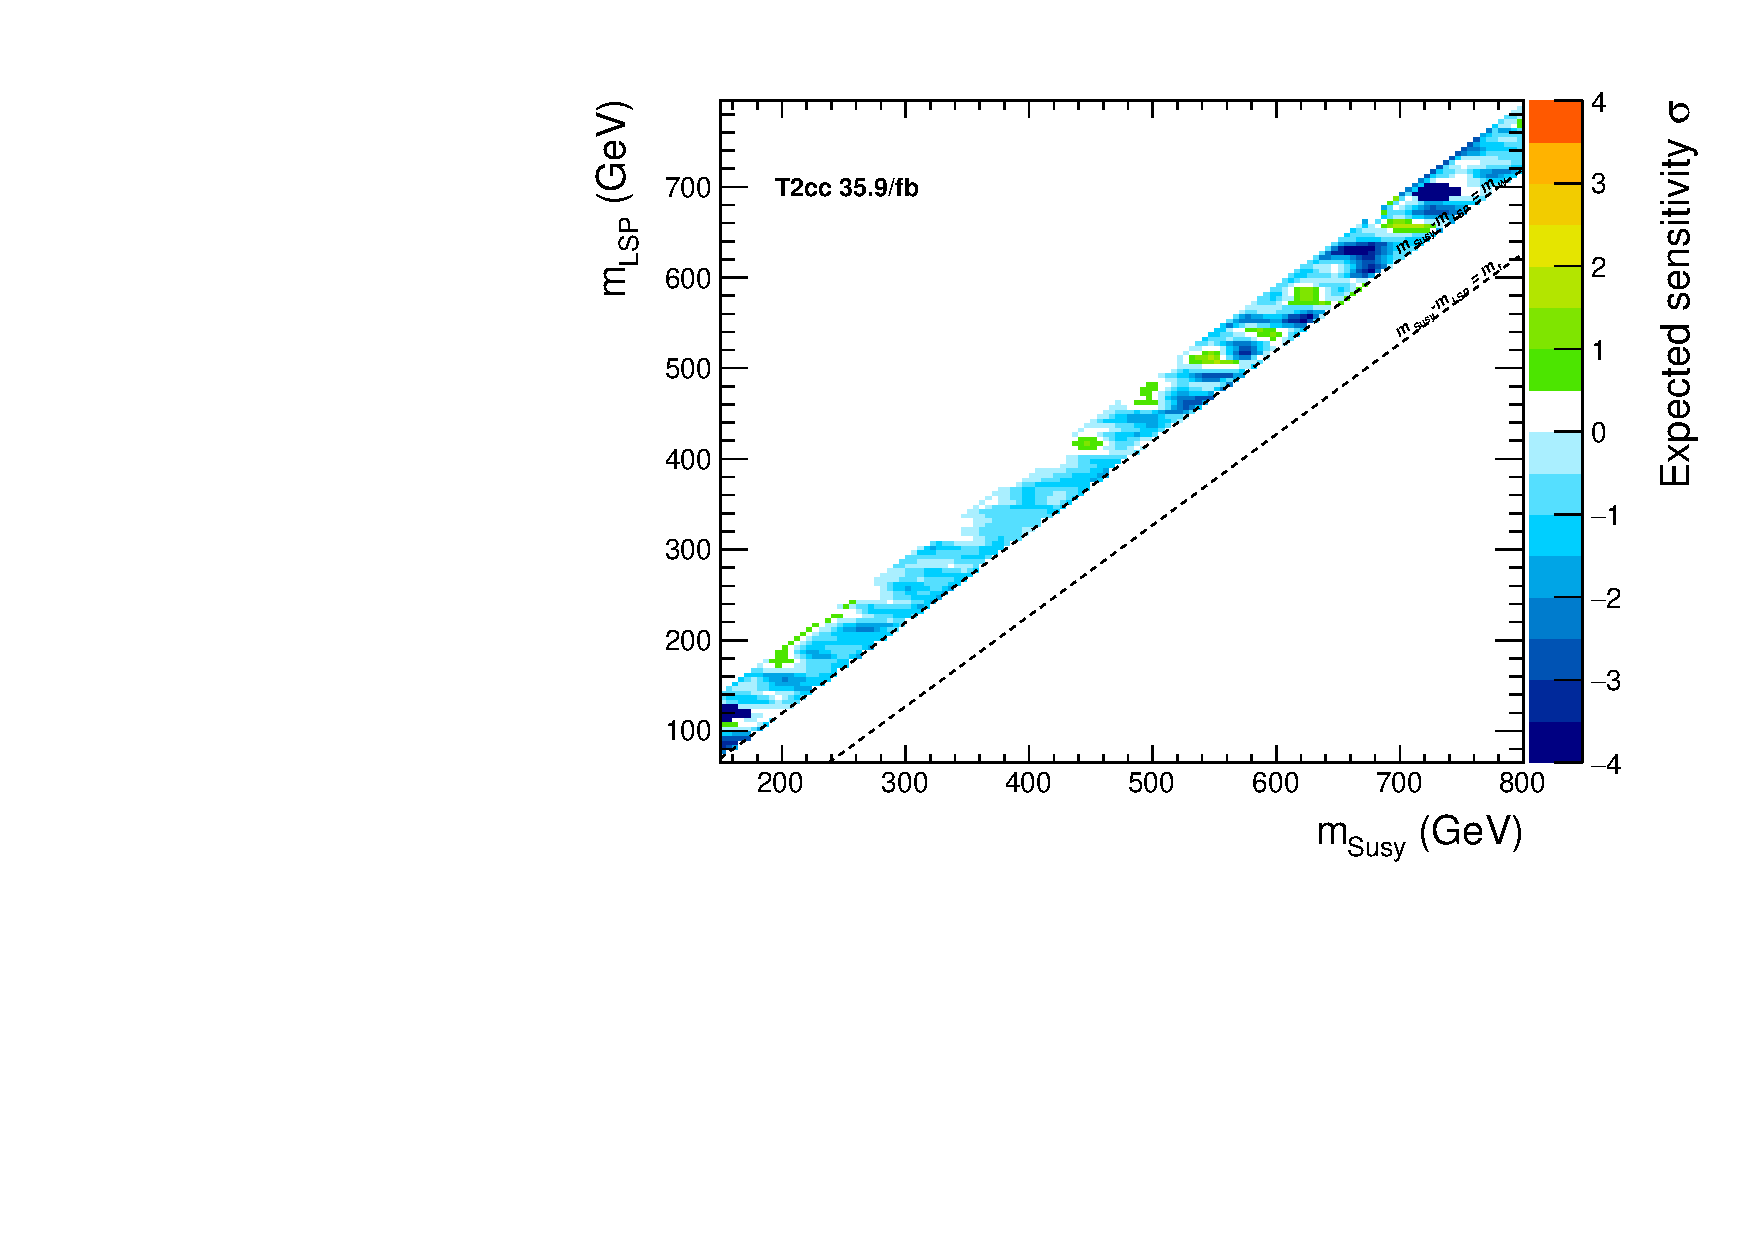
\includegraphics[width=0.45\linewidth]{figures/susyResults/T2cc_signif}
            \label{fig:T2cc_signif}
        } ~~
        \caption{Top: the 95\% C.L. observed upper limit on the cross section
            (histogram), with the expected (solid black line) observed
            (solid red line) exclusion contours. Left: signal acceptance
            including all jet categories. Right: graph showing the four
            most sensitive jet categories for each mass point. Bottom:
            local observed significance scan.
        }
        \label{fig:T2cc}
    \end{center}
\end{figure}


%\begin{figure*}[thp!]
%    \begin{center}
%        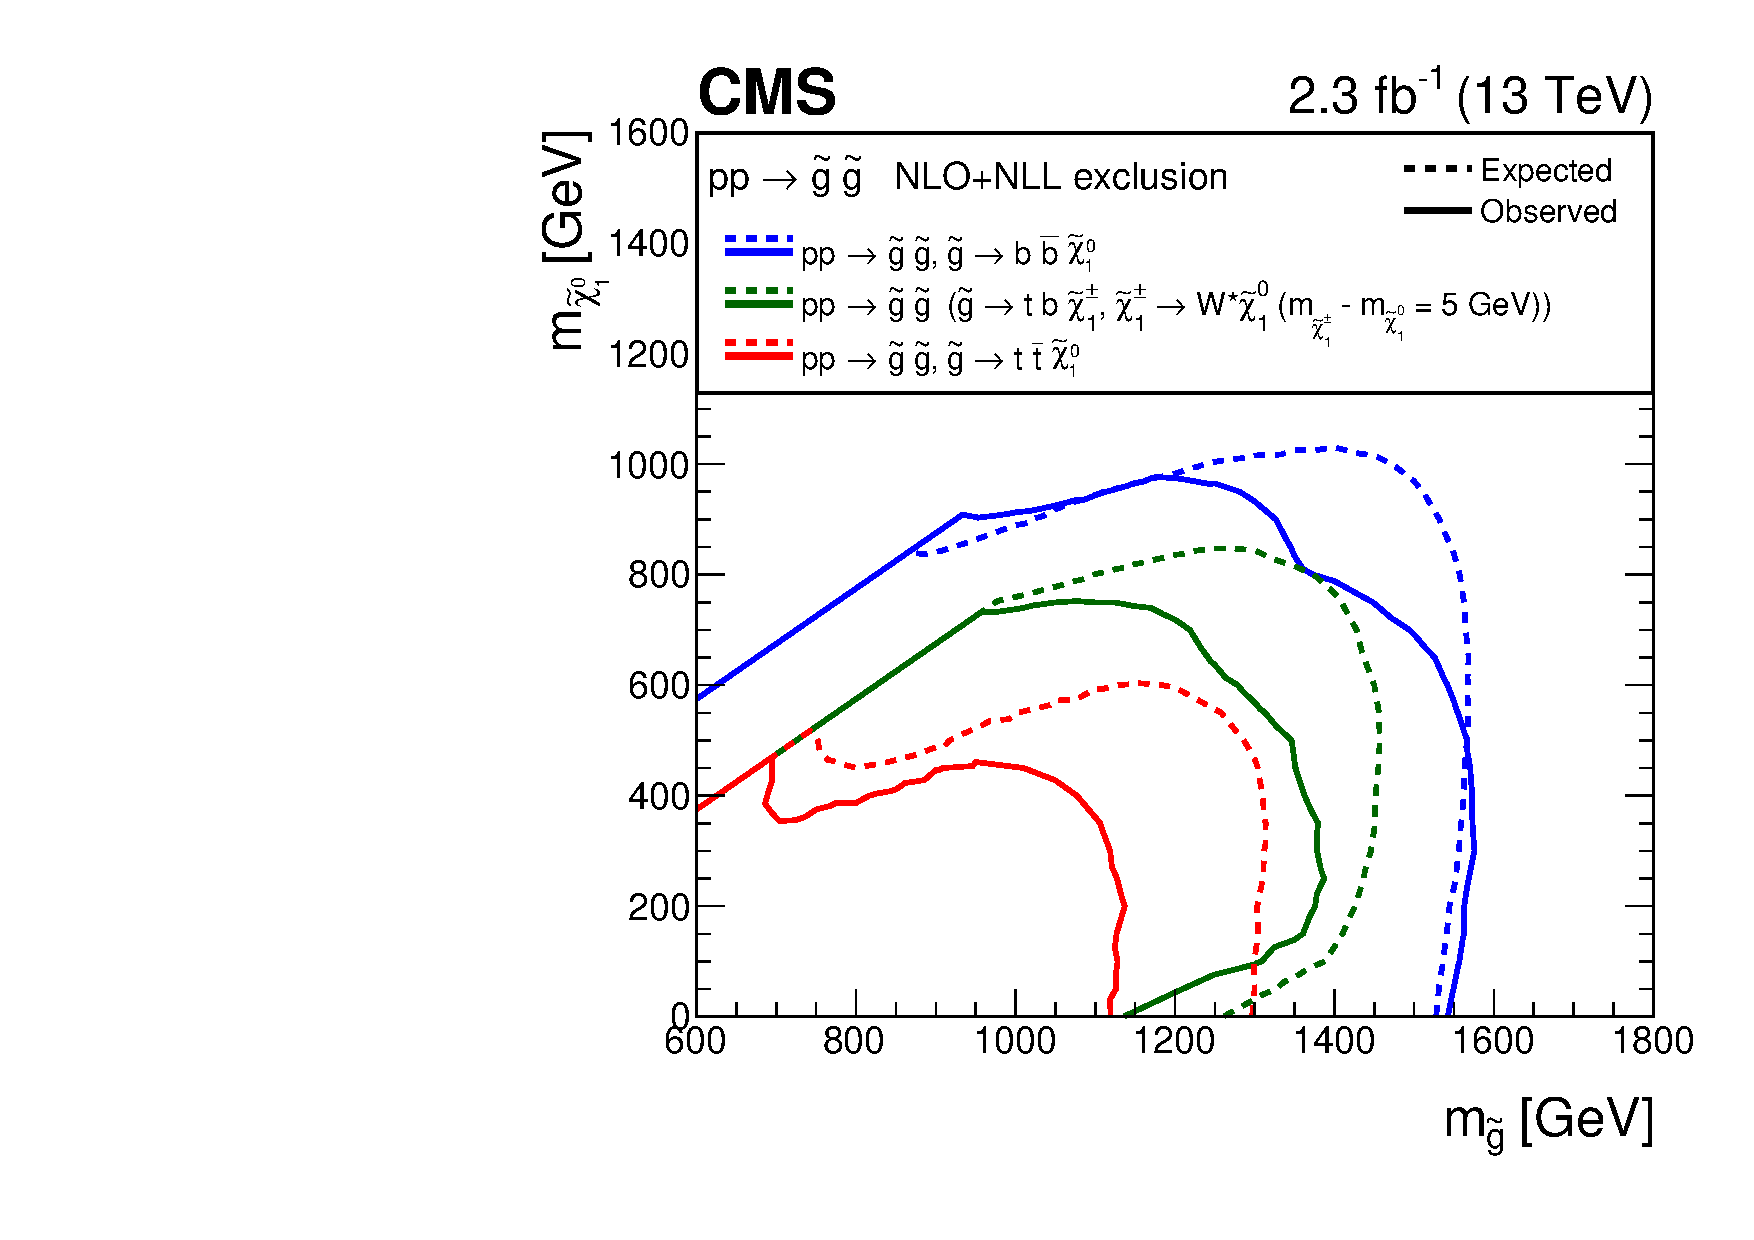
\includegraphics[width=0.49\textwidth]{figures/susyResults/gluinoSUMMARY.pdf} \\
%        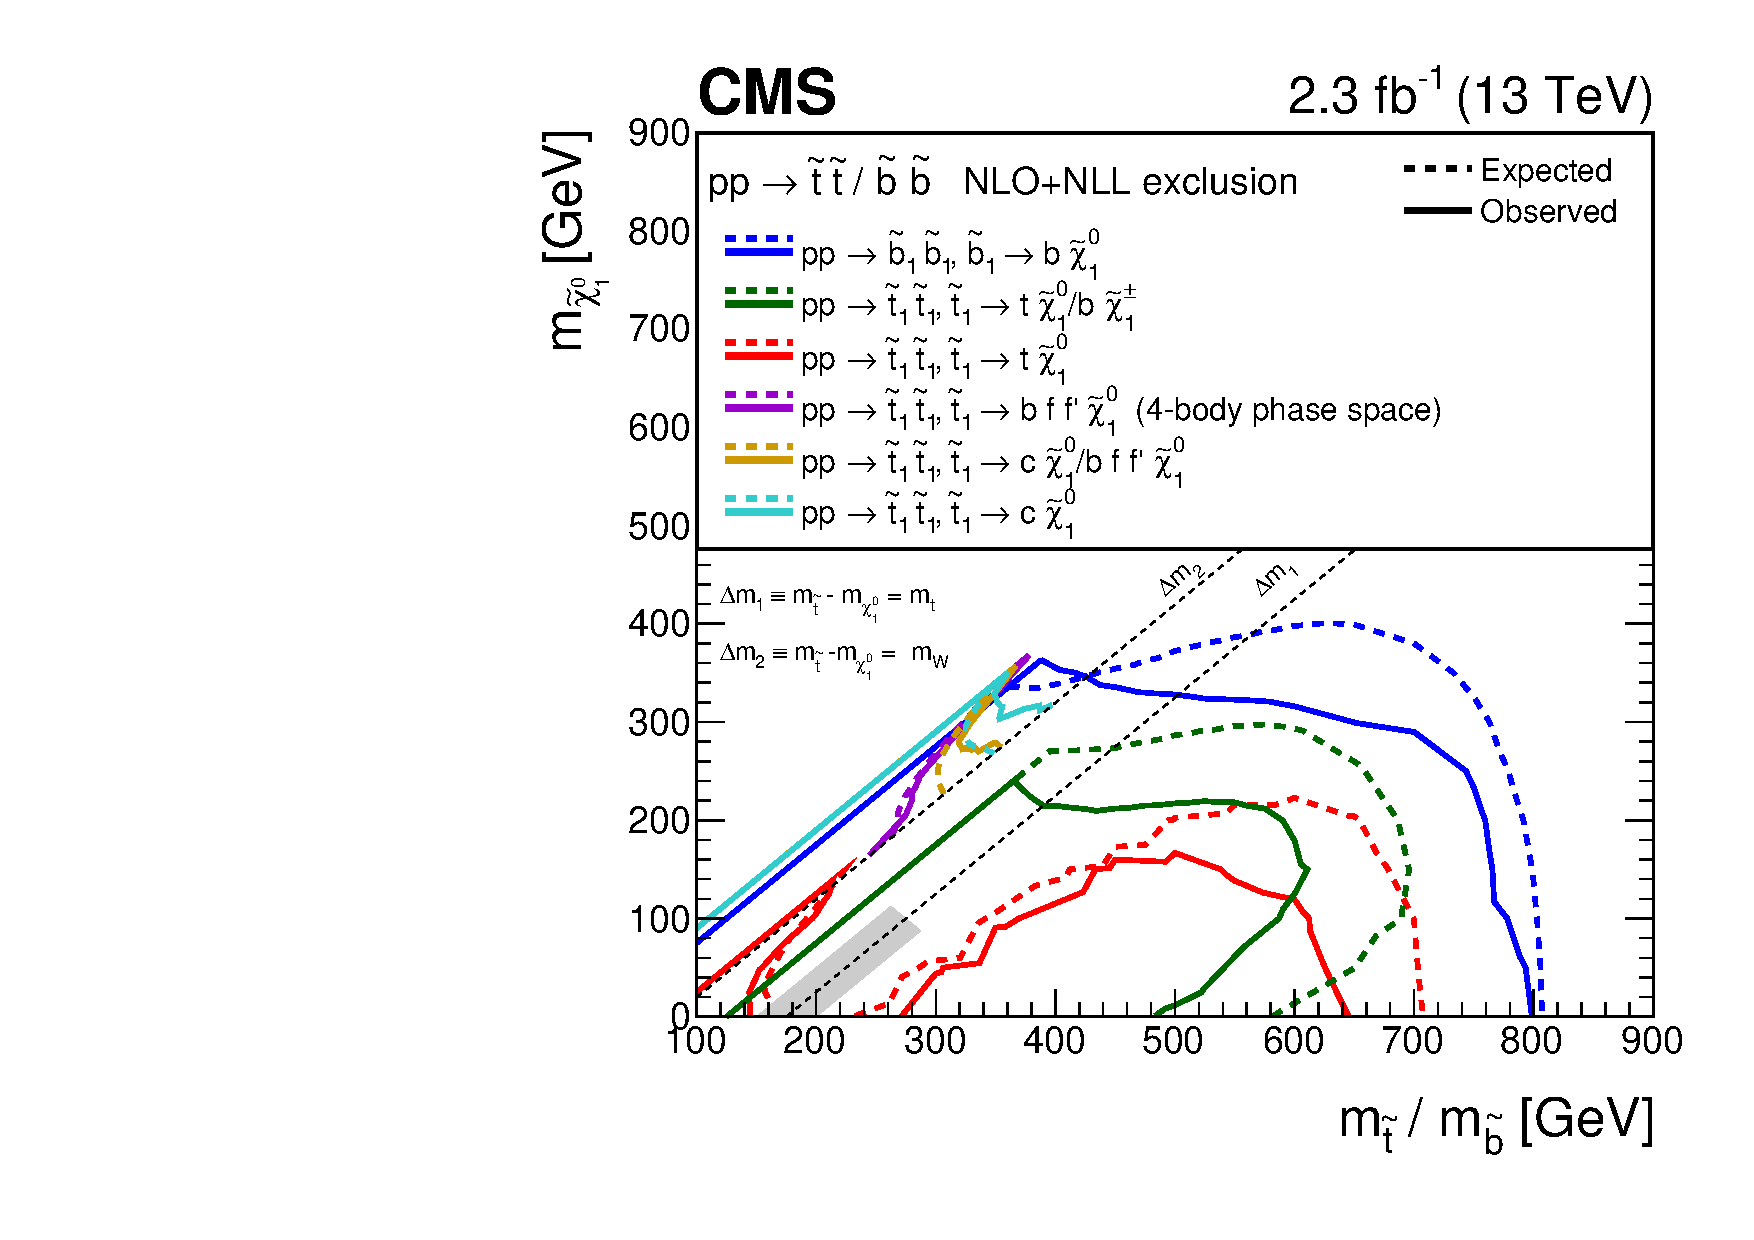
\includegraphics[width=0.49\textwidth]{figures/susyResults/allThirdGenSUMMARY.pdf} \\
%        \caption{Summary for the observed (solid lines) and expected
%            (dashed lines) exclusions in the $m_{\mathrm{Susy}},m_{\mathrm{LSP}}$
%            plane for the models considered in the analysis.Exclusion contours
%            are grouped into 4 summary plots according to the categorisation
%            presented at the begin of Sec.~\ref{sec:susy_results}:
%            ``Gluino-mediated production of off-shell (decoupled) 3rd generation
%                squarks'' (top right),
%            ``Direct production of 3rd generation squarks'' (bottom right).
%        \label{fig:summary-excl-plots} }
%    \end{center}
%\end{figure*}

\newpage
With expected limit, gluino masses up to $\sim$1800 GeV for the decay into
light-quarks (T1qqqq), $\sim$2050 GeV for the decay into b-qarks (T1bbbb) and
$\sim$1850 GeV for the decay into t-quarks (T1tttt). Squark production is
excluded up to squark masses $\sim$1400 GeV for the 8-fold models, and up to
$\sim$800 GeV for the 1-fold (degenerate) models (T2qq). Sbottom production is
excluded to sbottom masses $\sim$1100 GeV (T2bb).  Stop production is excluded
up to stop masses $\sim$1050 GeV in the 2-body decay to top quarks (T2tt), and
up to $\sim$550 GeV in the compressed region of decays into charm quarks (T2cc).
For the models considered, the exclusion exceeds the one of the 13 TeV ICHEP
data.

%%____________________________________________________________________________||
